\section{Characterization Problem Results}
\label{sec:CharResults}

To quantify the $\Omega$-method success for a variety of anisotropy-inducing
physics, we will present various forms of the Figure of Merit, as described in
Section \ref{sec:successmetrics}.
In the preceding subsections, a
subset of flux anisotropy-inducing physics have been identified
and a subset of problems that contain these physics have been conceived.
In this section, the results for CADIS-$\Omega$, CADIS, and analog Monte Carlo
will be presented for each of these problems. Explanations on the performance of
the $\Omega$-methods will accompany the results for each problem. In some cases,
variants of problems were run to confirm or refute observations seen
in other problems.

\subsection{Computational Specifications}
\label{subsec:comp_specs}

As noted in a number of the previous sections, hybrid methods require both a
deterministic and a Monte Carlo calculation to obtain a problem result. These
transport codes require different computational parameters to obtain an answer.
For the characterization problems the computational parameters are summarized in
Table \ref{tab:simulation_defaults}; the parameters for the deterministic and
Monte Carlo calculations are demarcated in the table.

\begin{table}[h!]
  \centering
  \begin{tabular}{l|m{5cm}}
\toprule
Parameter Type & Parameter Value \\
\midrule \midrule
\multicolumn{2}{c}{ADVANTG Values$^1$} \\
\midrule
P$_N$ Order               &    $3$ \\
Quadrature Type           &  Quadruple Range \\
Quadrature Order          &    $10$ \\
Spatial Solver            &  Step Characteristic \\
Energy Group Library$^{\dagger}$     &    27G19N \\
Boundary Conditions & vacuum \\
\midrule \midrule
\multicolumn{2}{c}{MCNP Values$^2$} \\
\midrule
Particle Count      &   $1e7$ \\
Boundary Conditions & vacuum \\
\bottomrule
\end{tabular}
\begin{flushleft}
\footnotesize{
  $^1$ ADVANTG runs of the characterization problems
  were run on 16 cores of a 32 core node, with 256Gb of memory on
  an Oak Ridge National Laboratory compute cluster maintained by the Radiation
  Transport and Nuclear Systems Division. \\
  $^2$ MCNP runs of the characterization problems were run on the same
 machine, with 256Gb of memory but using all 32 cores of the node. \\
  $^{\dagger}$ Parameter type that has no default in ADVANTG.}
\end{flushleft}


  \caption[Default simulation values for characterization problems.]{
    Default simulation values for the characterization problems. The values for
    ADVANTG primarily signify parameters used to run Denovo, with exceptions for
    calculating biasing parameters, which is done exclusively in ADVANTG.
    MCNP-specific values are those used for Monte Carlo runs.
  }
  \label{tab:simulation_defaults}
\end{table}

The first portion of the table summarizes the values used by ADVANTG. Note that
these values all pertain to the Denovo deterministic solver, which is set up by
ADVANTG. The parameter types marked with a dagger have no default in ADVANTG.
We have chosen to use a relatively course 27 group energy group library.
Because the characterization problems are meant to identify the method's
performance pertaining to flux anisotropy, and we expect the energy group
structure to have less of an effect on anisotropy conditions than other
parameters, we opted for a
computationally inexpensive energy group mesh for the deterministic solver.
Further, this group library was designed for radiation shielding applications,
so it applies to the majority of the characterization problems.

The boundary conditions for all of the characterization problems will be vacuum.
At this time, ADVANTG does not support reflective boundary conditions,
which is a limitation in application space that we cannot address at this
time. The Monte Carlo code we use does support vacuum boundary conditions, but a
discrepancy in boundary conditions between deterministic and Monte Carlo
calculations would result in a mismatch between the problem the biasing parameters
are for and the one we are trying to solve. 

Unless otherwise noted, the values in this subsection of the table are ADVANTG
default values. They are a good initial choice for characterization of the
method because they are often chosen as the parameters for hybrid methods studies
by experienced and inexperienced ADAVANTG users.
Further, these values are defaults in ADVANTG for their
computational stability, such as not having negative valued weights or fluxes,
stable convergence, a relatively fast time to a solution, et cetera. Due to
the good properties exhibited by the solver options and because users first
using the $\Omega$-methods are likely to choose these values, the values in
Table \ref{tab:simulation_defaults} will be used for the characterization of the
$\Omega$-methods.

The latter section of the table summarizes the Monte Carlo code MCNP values for
each of the problems. The value of $1e7$ particles as a particle cutoff
was chosen because it made the
error bins in the majority of the analog Monte Carlo
characterization problems less than 100\%. In some problems that are
extraordinarily difficult for Monte Carlo to solve without biasing, there were
tally bins with very high errors. In the following subsections, they will be
clearly indicated and their results will not be plotted so as to not obfuscate
the CADIS and CADIS-$\Omega$ results. Time cutoffs were not chosen because
we decided to measure how effective the $\Omega$-methods were at reducing the
variance per particle. Depending on the flux maps generated from CADIS and
CADIS-$\Omega$, the time to transport a finite number of particles may vary. As
a result, the reported times from a simulation can tell us whether the method
requires more sampling than other methods in addition to how fast it takes to
reach a desired relative error.

The responses in the NaI detectors of each of
the problems was measured with an MCNP track length tally (f4). The tally was
energetically binned to match the dataset of the multigroup dataset provided in
ADVANTG, and the entire volume of the detector was used with no spatial
binning. 

It should be noted that, while the tally is energetically binned, Monte
Carlo transport is not discretized in space or energy like deterministic
transport. In a nonbiased analog Monte Carlo calculation, transport is
completely continuous in space, energy, and angle. In a hybrid calculation using
VR parameters from a deterministic solution, the VR parameters will be
discretized to reflect the solution obtained from the deterministic solver. As a
result, the particle's transit throughout the
problem will be a combination of sampling both continuous and discretized-energy
dependent factors. Consider a particle that goes through a scattering event
in shielding material. In this scattering event, the particle samples from a
continuous-energy cross section and may change energy as a result of the interaction.
However, depending on how much energy the particle loses in the scattering event it may
cross into the energy range of a lower-energy weight window and will require
further sampling.

All characterization problems were run on Remus, a machine operated and
maintained by the Radiation Transport and Nuclear Systems Division at Oak Ridge
National Laboratory. The ADVANTG runs were run on 16 cores of a 32 core node,
with 256 GB of memory. The MCNP runs were run on the same machine, with 256 GB of
memory but using all 32 cores of the node. Monte Carlo and ADVANTG
inputs and directions on how to acquire them are
provided in Appendix \ref{sec:github_codes}.

%Each problem presented in Section \ref{sec:CharResults} will
%use the values specified in Table \ref{tab:simulation_defaults}
%unless otherwise noted.
% already stated
%Times to transport the Monte Carlo particle quantity varies between methods
%due to differences in sampling.
% seems obvious

% in all results tables, you might want to bold the best value and italicize the worst, or something similar, that makes it easeir to see. 
% or old the best for each horzontal category

\subsection{Single Turn Labyrinth}
\label{subsec:maze2}

The analysis of the characterization problems begins with the single turn
labyrinth.
The single turn labyrinth FOM results and runtimes are summarized in Table \ref{tab:maze2foms},
and are illustrated in Figures \ref{fig:maze2result} and \ref{fig:maze2error}.
 The equations to
calculate each of these FOMS is summarized in Table \ref{tab:fom_defaults}. As a reminder,
   The relative errors used are the tally average relative error, the tally maximum relative
  error, and the tally minimum relative error; the times are total walltimes for
  the Monte Carlo calculation and the sum of the hybrid method times, the
  deterministic transport time, and the Monte Carlo calculation time.

\begin{table}[h!]
  \centering
  \begin{tabular}{lrrrrr}
\toprule
{} & \multicolumn{2}{c}{CADIS}   & \multicolumn{2}{c}{CADIS-$\Omega$}  & analog \\
{} &    MC & MC$_{hybrid}$ &         MC & MC$_{hybrid}$ &     MC \\
\midrule
tally avg   &  18.6 &        14.9 &       2.36 &        1.56 &   17.4 \\
max RE      &  2.76 &        2.21 &      0.481 &       0.318 & 0.0857 \\
min RE      &   249 &         200 &        196 &         130 &    -- \\
time (mins) &  67.7 &        84.4 &        157 &         237 &   11.7 \\
\bottomrule
\end{tabular}

  \caption[Figure of Merit comparison for single turn maze.]{Figure of Merit
    comparison for single turn maze.}
  \label{tab:maze2foms}
\end{table}
% these are foms, except the bottom row, which is time? I'd state that. 

In all cases, the
CADIS FOMs are better than those obtained by CADIS-$\Omega$. The FOMs
calculated using the tally average relative error are better in the nonbiased
analog Monte Carlo than CADIS-$\Omega$ as well. However, this is a product of
two effects: the time for the analog to run the same particle count is far
shorter than either CADIS or CADIS-$\Omega$. As a result, to obtain the same
FOM, CADIS-$\Omega$ needs to have $R_1/R_2 = \sqrt{T_2/T_1}$ (this is from
taking a ratio of the FOMs) the tally average
relative error, or ~$0.27$. 
% this sentence seems to be missing some words?
Because this problem is highly scattering and many
low-energy particles can make it through the concrete labyrinth, even analog MC
can have good sampling at low energies, resulting in a tally average FOM that
reaches this threshold.

\begin{table}[h!]
  \centering
  \begin{tabular}{llrrr}
\toprule
          &              &          cadis &     cadisangle &         analog \\
          &              & time (minutes) & time (minutes) & time (minutes) \\
\midrule
MCNP time & total &          67.71 &         157.01 &          11.67 \\
deterministic time & advantg\_time &           0.26 &           0.28 &            -- \\
          & denovo\_time &          16.41 &          78.19 &            -- \\
          & dispose\_time &           0.01 &           0.40 &            -- \\
          & omega\_time &           0.00 &           1.61 &            -- \\
          & total &          16.67 &          80.08 &            -- \\
wall time &              &          84.38 &         237.09 &          11.67 \\
\bottomrule
\end{tabular}

  \caption[Detailed timing results for single turn maze.]
  {Detailed timing results for single turn maze.}
  \label{tab:maze2times}
\end{table}
% again, I'd put horizontal lines between the 3 categories.

Table \ref{tab:maze2times} contains more detailed timing information. 
We can see that the Monte Carlo
runtime for CADIS-$\Omega$ is more than twice that of CADIS, and almost fifteen
times that of the nonbiased analog Monte Carlo. The time to run just the
hybrid/deterministic portion of the calculation is also four times longer for
CADIS-$\Omega$ than it is for CADIS. These disparities in runtimes have a strong
negative impact on the CADIS-$\Omega$ FOMs.

\begin{figure}[h!]
  \centering
  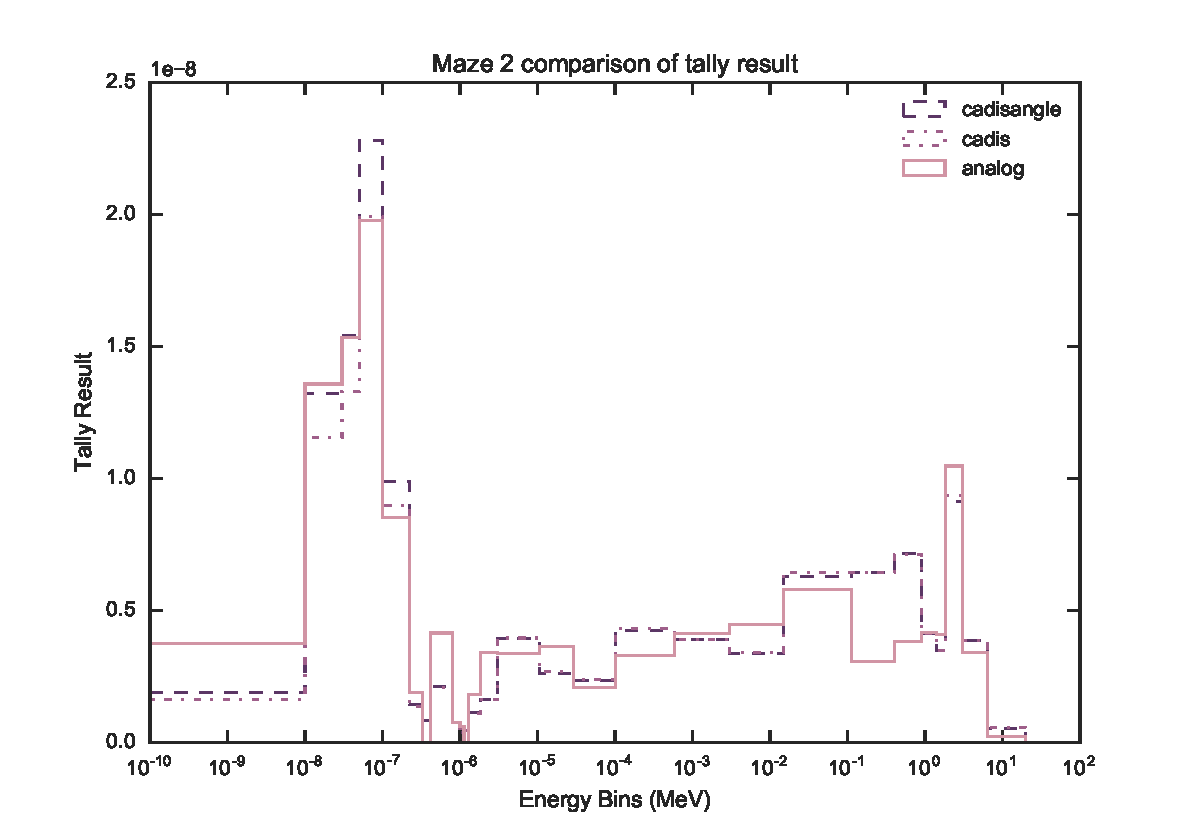
\includegraphics[height=10cm]{./chapters/characterization_probs/figures/char/maze2/maze_2_tally_result_compare.pdf}
  \caption[Tally results comparison between methods for single turn labyrinth.]
  {Tally results comparison between methods for single turn labyrinth.}
  \label{fig:maze2result}
\end{figure}
% if you end up needing to remake the plots, I'd take the titles off. You don't call this maze 2 anywhere else.
% I wouldn't change it now, but for papers, the future, etc.

\begin{figure}[h!]
  \centering
  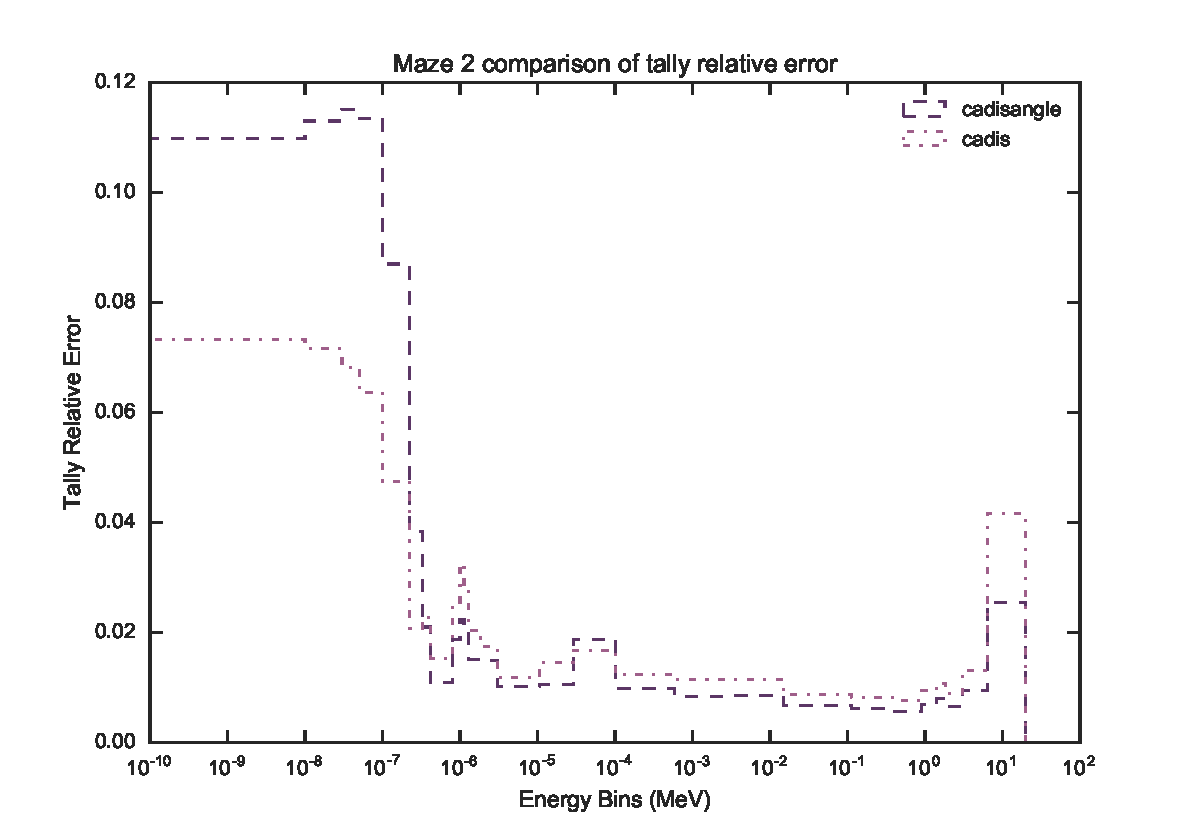
\includegraphics[height=10cm]{./chapters/characterization_probs/figures/char/maze2/maze_2_tally_error_compare.pdf}
  \caption[Tally relative error comparison between methods for single turn
  labyrinth]{Tally relative error comparison between methods for a single turn
  labyrinth.}
  \label{fig:maze2error}
\end{figure}

Figures \ref{fig:maze2result} and \ref{fig:maze2error} show the tally results and
the relative errors for the single turn maze, respectively.
The relative error plot,
Figure \ref{fig:maze2error}, does not include the
relative error bins of the analog result because they are significantly higher
than the CADIS and CADIS-$\Omega$ results. This is further confirmed in Table
\ref{tab:maze2foms}, where the minimum relative error FOM is a non-tallied bin.

By inspecting Figure \ref{fig:maze2result}, one can observe that the CADIS and
CADIS-$\Omega$ results are in agreement in bins greater that $10^{-7}$ MeV. At
lower energy bins, CADIS-$\Omega$ generally has a higher value for the tally
result than standard CADIS. However, in comparing the errors for these low energy
bins in Figure $\ref{fig:maze2error}$, CADIS has a lower relative error. This
indicates that CADIS sampled many more low-weight particles than CADIS-$\Omega$
in these regions. Conversely, CADIS-$\Omega$ has a lower relative
error than CADIS for bins greater than $\sim5*10^{-6}$ MeV. This is expected, as
higher energy particles generally exhibit a stronger angular dependence than
low-energy particles. In geometric and energetic regions
where the angular dependence is stronger,
the importance map generated by CADIS-$\Omega$ may show more of an effect in
improving the relative error.

To aid in our understanding of how the $\Omega$-methods' importance map differs
from the standard adjoint flux map, let us compare the flux distributions
obtained by different deterministic solutions of the single turn labyrinth.
Figure \ref{fig:maze2fluxmaps} shows several different flux distributions that
represent the single turn labyrinth geometry. This figure is of the highest
energy group for each flux type. The flux maps have scales normalized to maximum and minimum values
  for each slice; between plots the scales are not consistent. 

% the figure numbers don't seem to be displaying correctly. I'd make them all separate figure #s b/c they are split over multiple pages. 
\begin{figure}[htb!]
  \centering
  \begin{subfigure}[t]{\textwidth}
    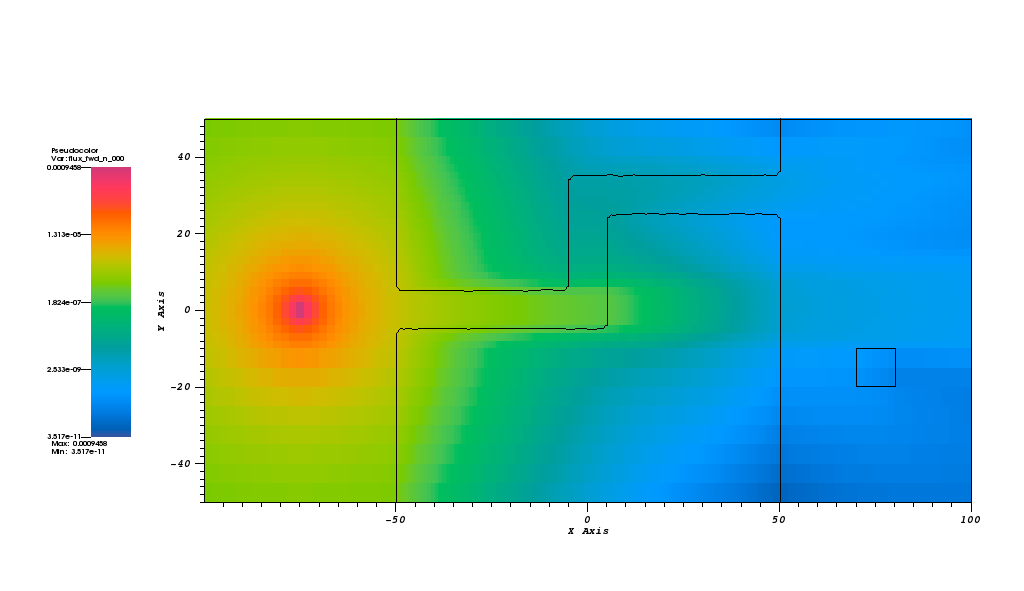
\includegraphics[width=0.9\linewidth]{./chapters/characterization_probs/figures/char/maze2/maze2MfwdG00.png}
    \caption{Forward flux map for highest energy group, single turn
    labyrinth.}
    \label{fig:maze2fwd}
  \end{subfigure}
\end{figure}
\begin{figure}[htb!]\ContinuedFloat
  \centering
  \begin{subfigure}[t]{\textwidth}
    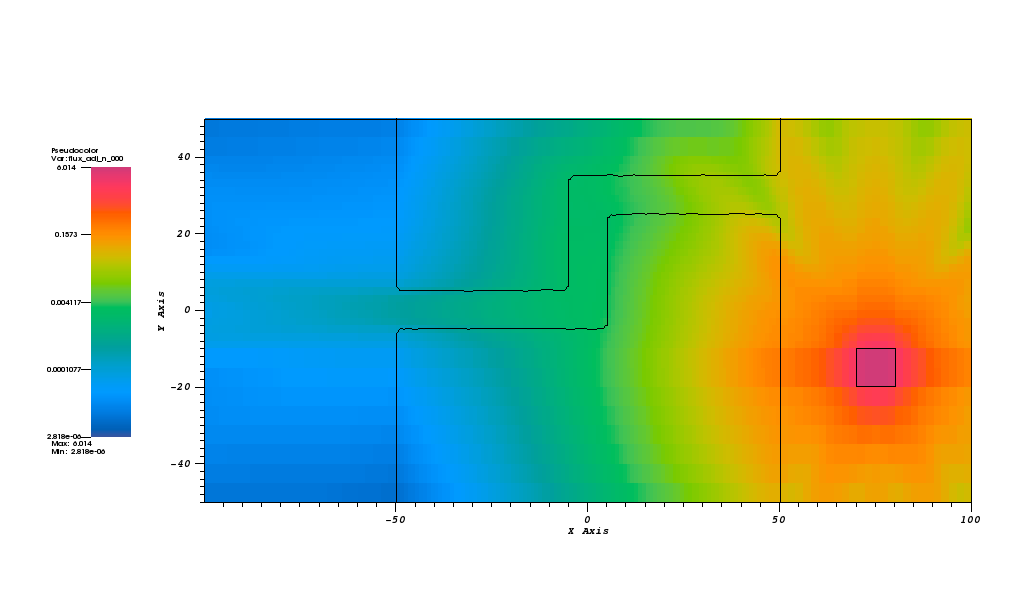
\includegraphics[width=0.9\linewidth]{./chapters/characterization_probs/figures/char/maze2/maze2MadjG00.png}
    \caption{Adjoint flux map for highest energy group, single turn
    labyrinth.}
    \label{fig:maze2adj}
  \end{subfigure}
\end{figure}
\begin{figure}[htb!]\ContinuedFloat
  \centering
  \begin{subfigure}[t]{\textwidth}
    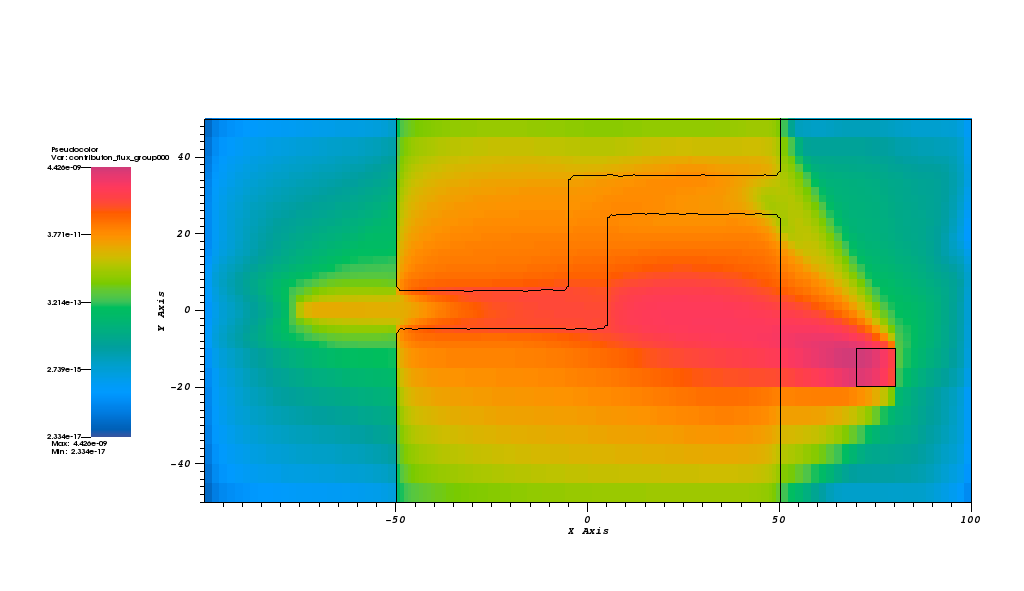
\includegraphics[width=0.9\linewidth]{./chapters/characterization_probs/figures/char/maze2/maze2McontribG00.png}
    \caption{Contributon flux map for highest energy group, single turn
    labyrinth.}
    \label{fig:maze2contrib}
  \end{subfigure}
\end{figure}
\begin{figure}[htb!]\ContinuedFloat
  \centering
  \begin{subfigure}[t]{\textwidth}
    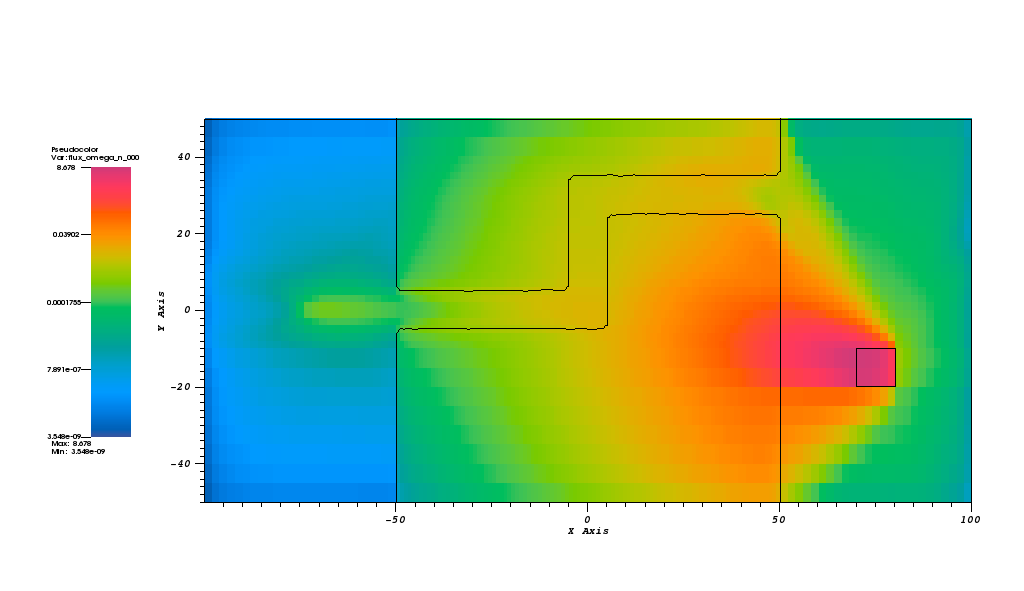
\includegraphics[width=0.9\linewidth]{./chapters/characterization_probs/figures/char/maze2/maze2MomegaG00.png}
    \caption{$\Omega$-flux flux map for highest energy group, single turn
    labyrinth.}
    \label{fig:maze2omega}
  \end{subfigure}
  \caption[Flux map slice of single turn labyrinth.]{}
  \label{fig:maze2fluxmaps}
\end{figure}

Figure \ref{fig:maze2fwd} shows the forward flux for the labyrinth. It is
clear that in this problem, particles emanate isotropically from the
source on the left side of the problem. Some particles travel towards the
shield and enter the labyrinth. After 50 cm some of these particles hit the wall in
the first turn of the labyrinth. Many high energy particles reach fairly deep
into the concrete past this turn.

Figure \ref{fig:maze2adj} complements Figure \ref{fig:maze2fwd} by showing the
adjoint scalar flux distribution for the fastest energy group. Recall that this
distribution is what is used by CADIS to generate VR parameters. Particles are
generated throughout the NaI detector and exit the detector in all directions.
Because the source is not in line with the labyrinth entrance, particles end up
colliding much closer to the labyrinth edge than in the forward distribution.
There also exist some prominent ray effects in this distribution on the right
hand side of the problem. In particular, the contrasting orange and green
fingers of the ray effects show at least an order of magnitude change in the
flux for forward particles exiting the maze in this region. In reality, the
importance in this region should be close to a spherical surface some distance
away from the adjoint source.

Recall that the $\Omega$-flux is computed using the angle-integrated contributon
flux in the numerator. 
%For this problem, the contributon flux will be used to
%illustrate how the $\Omega$-flux is a combination of the adjoint and the
%contributon flux.
% that sentence doesn't make sense.
 Figure \ref{fig:maze2contrib} shows the distribution of
angle-integrated contributon flux values for the single turn labyrinth.
Interestingly, because so many forward particles penetrated deeply into the
shield, the contributon flux points directly into this section of the shield. It
is also clear that near the forward source, only particles moving 
towards the labyrinth entrance contribute to the contributon flux.
In the left-side of the labyrinth, we can observe directional importance in the
labyrinth channels, but in the first turn this directional importance is no
different than the concrete barriers surrounding the channels.

Figure \ref{fig:maze2omega} shows how the $\Omega$-flux is built from the
adjoint and contributon fluxes by showing the $\Omega$-flux distribution for the
single turn labyrinth. Comparing this figure to \ref{fig:maze2contrib}, the
majority of high flux regions are pushed back towards the NaI detector. The
flux gradient exiting the maze does not span as many orders of magnitude as it
did in the contributon flux plot. Further, the importance of particles does
not remain as high or go as deep into the concrete shield as the contributon
flux plot. This is because the $\Omega$-flux is normalized by the forward flux,
resulting in reducing importance in regions where only the forward flux is
strong. As with the contributon flux, the $\Omega$-flux strongly reduces
particle importance near the problem boundaries. Recall from Section
\ref{sec:ContributonImportance} that in the contributon transport equation
the cross section becomes very high near problem boundaries, thus encouraging
particles back towards the problem source and sink. Because the $\Omega$-flux
uses standard forward and adjoint transport, the cross section is not
manipulated. However, the flux magnitude reflects importance consistent with
contributon theory.

Both the $\Omega$- and the contributon fluxes show a mitigation of ray effects
on the right hand side of the problem. Note that there are no ``fingers'' of
flux magnitude at distances several cm away from the NaI detector on the right
side of the problem in either Figure \ref{fig:maze2contrib} or
\ref{fig:maze2omega}. Reducing these numerical apparitions is a positive effect
of the method. However, there exists a fairly strong gradient in flux magnitude
for a particle traveling directly out of the maze exit. As a result, a particle
traveling several cm of distance across this strong gradient line may move from
a region of very low importance to very high importance, causing 
significant sampling requirements for the $\Omega$-importance that may not exist
with the standard adjoint.

A description of filtering algorithms accompanied
the discussion of the anisotropy metrics in Section
\ref{subsec:resultsintro}. The filtering algorithms are based on the contributon
flux distribution in the problem. Recall that the two
filter matrices include the cells where the contributon flux
is above the average contributon flux value. For the single-turn labyrinth, the filter matrix in the
highest energy group (Figure \ref{fig:maze2contrib}) will use values in the
orange and pink region of the figure and exclude values from the blue and green
regions of the figure. As a result, only anisotropy metric values from within
the maze will be used. The very anisotropic values near the edge of the problem
(where significant particle streaming exists), will not be included because they
are likely to be inconsequential to the tally response.

\begin{figure}[h!]
  \centering
    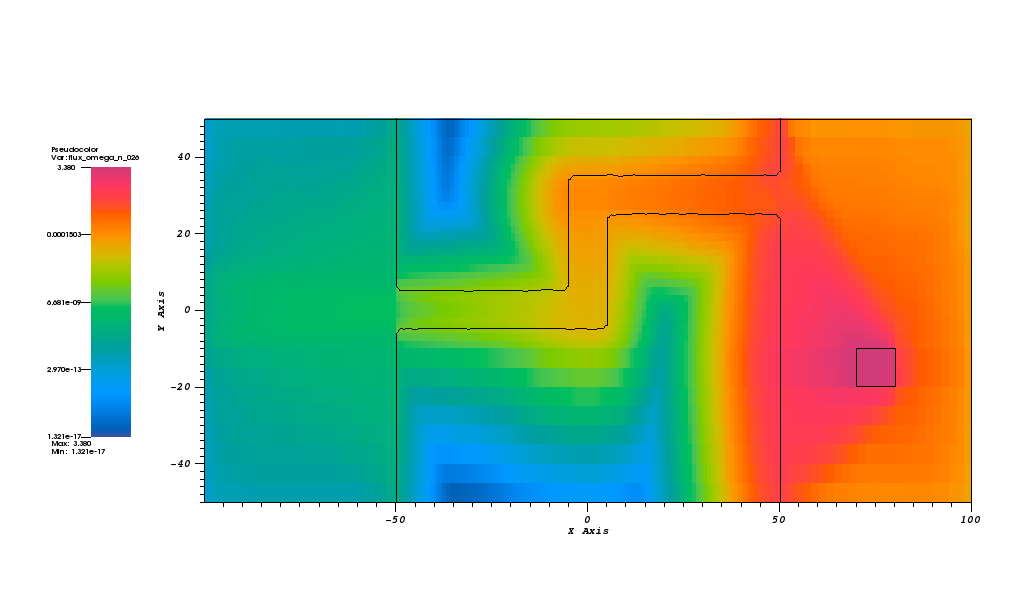
\includegraphics[width=0.9\linewidth]{./chapters/characterization_probs/figures/char/maze2/maze2MomegaG26.png}
    \caption{$\Omega$-flux flux map for lowest energy group, single turn
    labyrinth.}
    \label{fig:maze2omega26}
\end{figure}

Figure \ref{fig:maze2omega26} shows the $\Omega$-flux distribution for the
lowest energy group. This differs quite a bit from Figure \ref{fig:maze2omega} in that
the flux in the labyrinth has a much stronger gradient once entering concrete
than the higher energy group. This is expected, as the mean free path of a low
energy neutron is much shorter than a high energy one, especially in a dense,
hydrogenous material like concrete. As a result of the stronger flux gradient in
concrete, low energy particles entering
the concrete shield will be rouletted at a much greater frequency than high
energy particles. Low energy particles exiting the labyrinth also see a smaller gradient of
importance than the high energy particles do. As a result,
particle splitting and rouletting in this air region will be less extreme at low
energies than at high energies.

Comparing the $\Omega$-fluxes in Figures \ref{fig:maze2omega} and
\ref{fig:maze2omega26}, we can start to explain some of the timing behavior
observed in Tables \ref{tab:maze2foms} and \ref{tab:maze2times}.
High energy particles exiting the maze towards the 
detector have much longer mean free paths than the low energy particles, and
will generally have a much larger contribution to the $\Omega$-flux in those
regions. This is illustrated in Figure \ref{fig:maze2omega}.
The shape of the $\Omega$-flux 
around the detector region is much more dependent on direction in
the high energy group than it is for the lower energy group.
Despite having lower relative errors than CADIS at higher energies,
CADIS-$\Omega$ has lower FOMs than CADIS for the
minimum relative error. As discussed previously, this is due to the long runtime
of CADIS-$\Omega$, which is more than twice as long as CADIS. From this, we can
conclude that while CADIS-$\Omega$ is better at transporting particles in high
energy regions than CADIS, achieving lower relative errors, the length of time
to do so is prohibitive.
% a big punchline out of all of this may end up being that FW-CADIS-\Omega is really worth
% investigating b/c the determ transport times will become equitable. 
% It may also be that we just need way bigger problems st the determ transport time
% washes out in comparison with MC time. It's too bad that for these problems the
% MC time is comparatively short. 

\subsection{Multiple Turn Labyrinth}
\label{subsec:maze1}

The multiple turn labyrinth materials are the same as the single turn, but the geometry differs. Table
\ref{tab:maze1foms} summarizes the FOMs and runtimes. Figures \ref{fig:maze1result} and
\ref{fig:maze1error} show the results obtained by the track length tally for each
method.

\begin{table}[h!]
  \centering
  \begin{tabular}{lrrrrr}
\toprule
{} & cadis &             & cadisangle &             & analog \\
{} &    MC & MC\_adjusted &         MC & MC\_adjusted &     MC \\
\midrule
tally avg   &   327 &         248 &        224 &          71 &  0.054 \\
max RE      &  1.46 &        1.11 &       1.02 &       0.322 & 0.0393 \\
min RE      &   113 &        85.6 &         71 &        22.5 &    -- \\
time (mins) &  51.5 &          68 &       35.5 &         112 &   25.5 \\
\bottomrule
\end{tabular}

  \caption[Figure of Merit comparison for multiple turn labyrinth.]{Figure of Merit
    comparison for multiple turn labyrinth.}
  \label{tab:maze1foms}
\end{table}

\begin{table}[h!]
  \centering
  \begin{tabular}{llrrr}
\toprule
          &              &          cadis &     cadisangle &         analog \\
          &              & time (minutes) & time (minutes) & time (minutes) \\
\midrule
MCNP time & total &          51.52 &          35.55 &          25.46 \\
deterministic time & advantg\_time &           0.25 &           0.21 &            -- \\
          & denovo\_time &          16.28 &          74.85 &            -- \\
          & dispose\_time &           0.01 &           0.40 &            -- \\
          & omega\_time &           0.00 &           1.74 &            -- \\
          & total &          16.53 &          76.80 &            -- \\
wall time &              &          68.05 &         112.35 &          25.46 \\
\bottomrule
\end{tabular}

  \caption[Detailed timing results for multiple turn labyrinth.]
  {Detailed timing results for multiple turn labyrinth.}
  \label{tab:maze1times}
\end{table}

In Tables \ref{tab:maze1foms} and \ref{tab:maze1times}
it is notable that the MC part of the CADIS-$\Omega$ runtime is
shorter than with CADIS. This differs from most of the other
test cases. However, it is also notable that the
deterministic time is much longer for CADIS-$\Omega$ than CADIS.

Table \ref{tab:maze1foms} shows that both CADIS and CADIS-$\Omega$ outperform
analog MC by a factor of $10^2$ or $10^3$, indicating the necessity of variance
reduction for a problem like this. In comparing the FOMs, CADIS slightly outperforms
CADIS-$\Omega$ for all relative errors, meaning that the time
to reach any relative error will be achieved faster by CADIS.

\begin{figure}[h!]
  \centering
  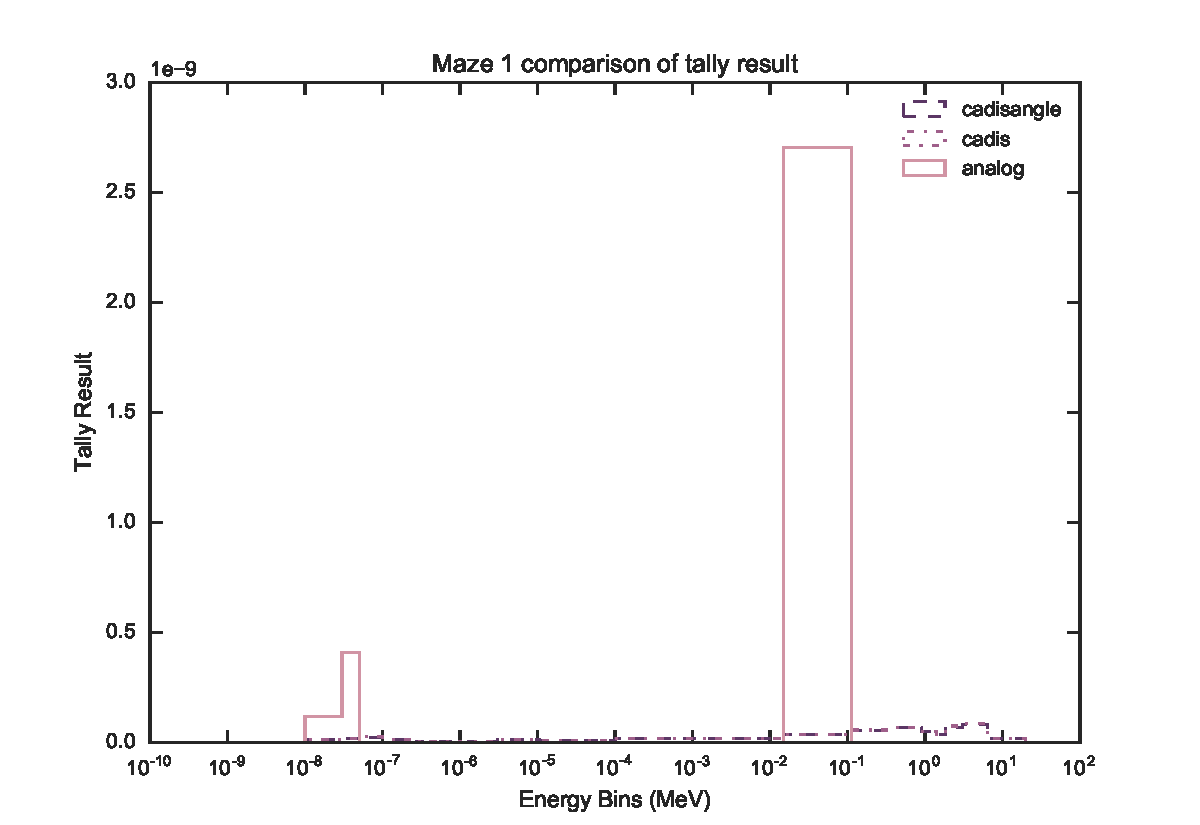
\includegraphics[height=10cm]{./chapters/characterization_probs/figures/char/maze1/maze_1_tally_result_compare.pdf}
  \caption[Tally results comparison between methods for multiple turn labyrinth.]
  {Tally results comparison between methods for multiple turn labyrinth. }
  \label{fig:maze1result}
\end{figure}
% can you make this log-log? It's really though to see the CADIS matchin.

\begin{figure}[h!]
  \centering
  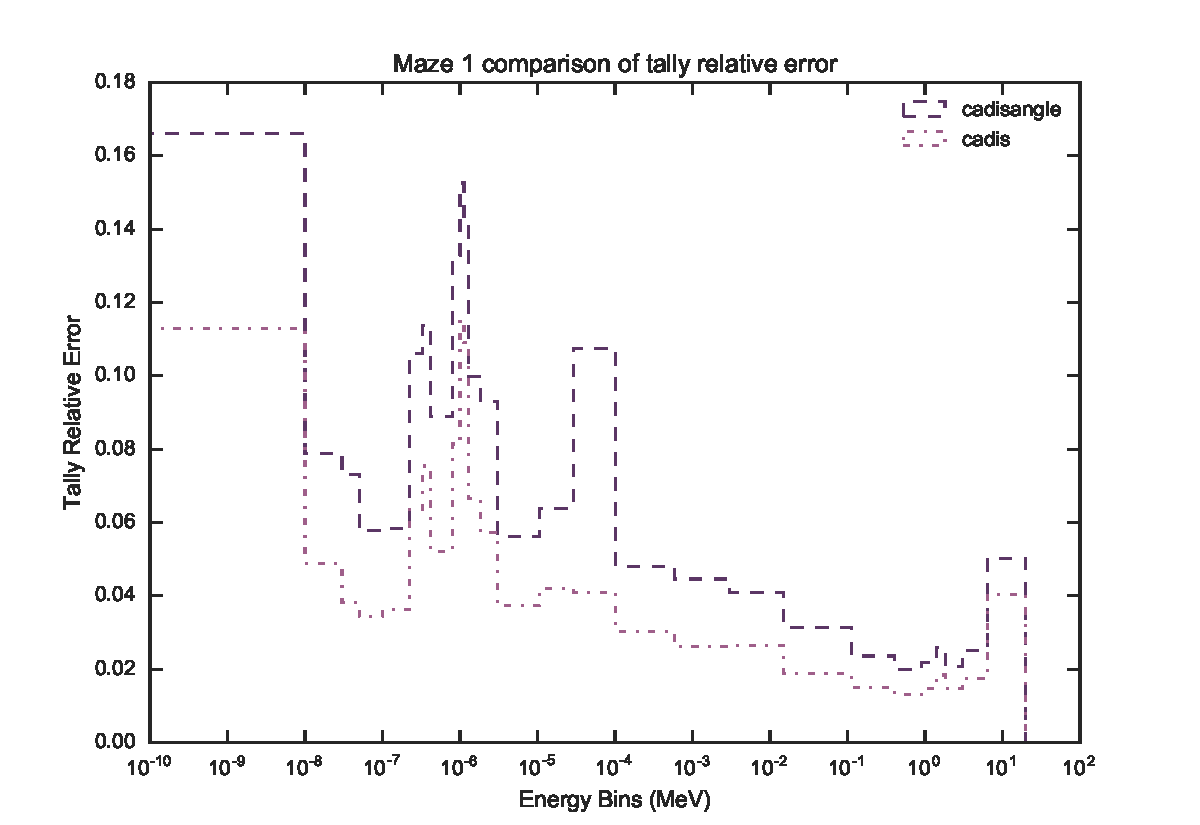
\includegraphics[height=10cm]{./chapters/characterization_probs/figures/char/maze1/maze_1_tally_error_compare.pdf}
  \caption[Tally relative error comparison between methods for multiple turn labyrinth]
  {Tally relative error comparison between methods for a multiple turn
  labyrinth. }
  \label{fig:maze1error}
\end{figure}

Looking at Figures \ref{fig:maze1result} and \ref{fig:maze1error}, we can see
that the analog Monte Carlo results differ significantly from either CADIS or
CADIS-$\Omega$. Two distinct regions of tally bins have been recorded in the
analog case: a high energy region comprised of particles that have scattered
very few times before reaching the detector, and a much smaller low energy
region, comprised of particles that are very thermal. These thermal particles
have a very small mean free path in the concrete labyrinth, thus the majority of them were
absorbed in the shield. However, given the errors on this result, these results are
not trustworthy. In the case of this problem, some of what was discussed in the
single-turn labyrinth is confirmed. This particular case requires that particles
scatter several more times if they are to exit the labyrinth from the air duct.
As a result, the spectrum is more thermal than the first case and the problem
has less anisotropy from the scattering effects.
As discussed in the single-turn labyrinth subsection, CADIS
outperformed CADIS-$\Omega$ in problems in energy bins that had less angular
dependence. Because this problem has far more scattering event, it overall has
less angular dependence and CADIS outperforms CADIS-$\Omega$ in all energy bins.
This problem is poorly suited to CADIS-$\Omega$.
% I'm not sure it's worth showing analog results. They tally plots don't have error bars,
% and if the analog results have really high error they're probably not worth showing. 

% same feedback about breaking up figures and putting caption in the text.
\begin{figure}[htb!]
  \centering
  \begin{subfigure}[t]{\textwidth}
    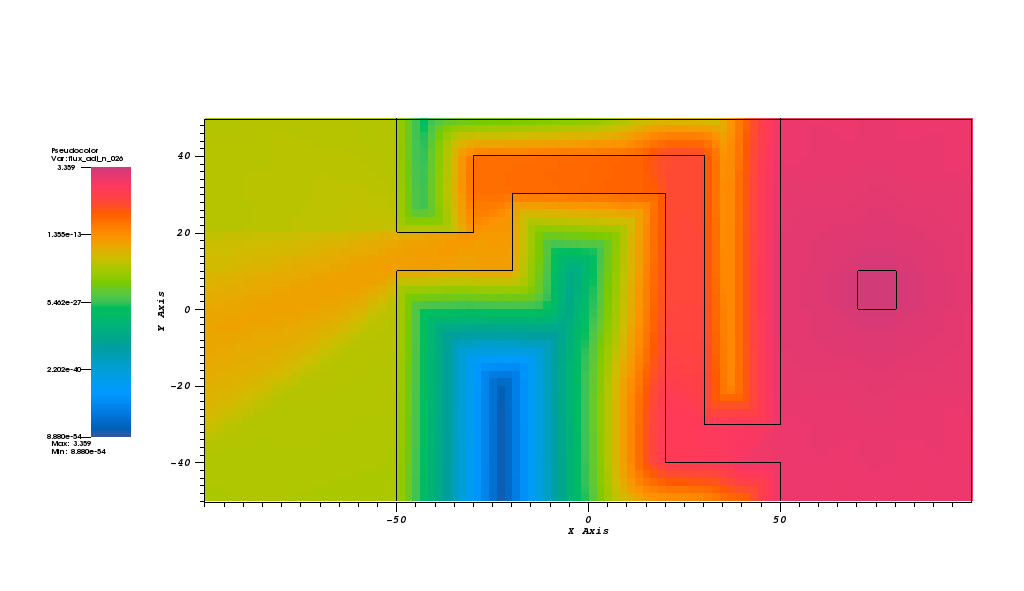
\includegraphics[width=0.9\linewidth]{./chapters/characterization_probs/figures/char/maze1/maze1adjG26.png}
    \caption{Adjoint flux map for lowest energy group, multiple turn
    labyrinth.}
    \label{fig:maze1adj}
  \end{subfigure}
\end{figure}
\begin{figure}[htb!]\ContinuedFloat
  \centering
  \begin{subfigure}[t]{\textwidth}
    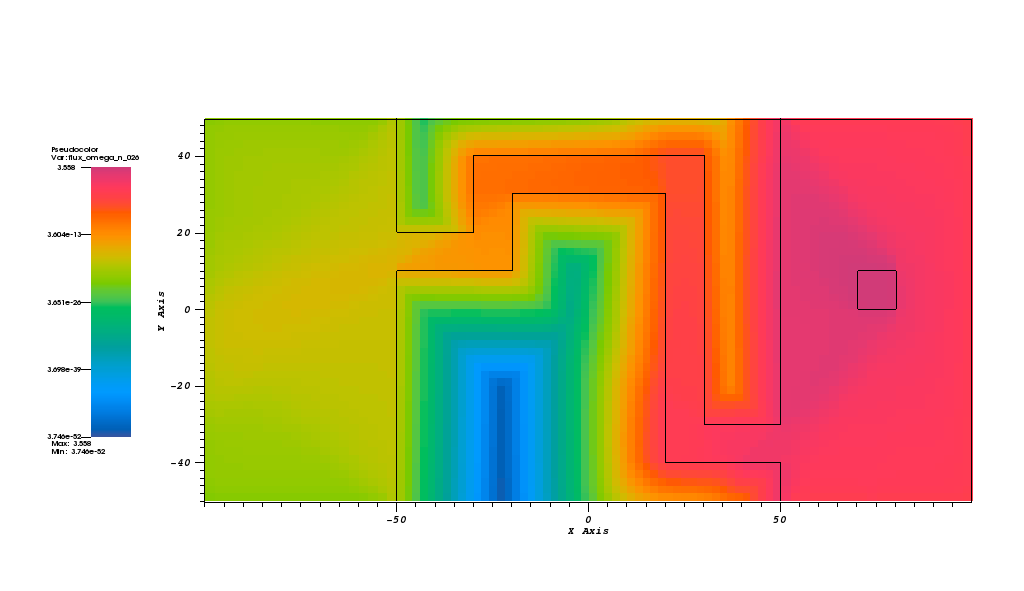
\includegraphics[width=0.9\linewidth]{./chapters/characterization_probs/figures/char/maze1/maze1omegaG26.png}
    \caption{$\Omega$-flux map for lowest energy group, multiple turn
    labyrinth.}
    \label{fig:maze1omega}
  \end{subfigure}
  \caption[Flux map slice of multiple turn labyrinth.]{Flux map slice of
    multiple turn
  turn labyrinth. Flux maps have scales normalized to maximum and minimum values
  for each slice; between plots the scales are not consistent. These plots show
  the lowest energy group for each cell in the problem midplane.}
  \label{fig:maze1fluxmaps}
\end{figure}

Figure \ref{fig:maze1fluxmaps} shows the adjoint and $\Omega$-flux maps for the
lowest energy group at the problem midplane.
These figures look remarkably similar, showing that this problem does not have
significant anisotropy to capture. The region that does differ is near the
detector, where the high importance is focused towards the
labyrinth and the laybrinth exit. The other region with noticeable difference is
located at the entrance to the maze. These figures show the lowest energy group
particles, so for forward particles of this energy to go the same direction as
adjoint particles, they must have gone into the labyrinth, scattered back out,
and then scattered again. As a result, we do not see a strong directional
dependence in the $\Omega$-flux plot in the region near the forward source. The
adjoint flux plot shows more of a streaming effect from the adjoint particles
that exit the maze.

\subsubsection{Labyrinth Comparison}
In Section \ref{subsec:maze2}, it was discussed that higher energy regions that
contribute to the tally are more anisotropic, and that these regions benefit
more from the $\Omega$-flux map than they do with a standard CADIS importance
map. Using the anisotropy metrics from Section \ref{sec:anisotropy_quant}, let
us compare the anisotropy distributions of the single turn and multiple-turn
labyrinth problems. Figure \ref{fig:labyrinthviolins} shows violin plots of the
M$_{3}$ distributions of the labyrinth problems. To filter out values of the
metric that do not have a strong contribution to the
tally, only values from cells above the contributon flux mean value are included
in the violins.

% Here is where I would put the explanation of how to read these. 

First, looking at the M$_{3}$ distributions for both the single-
(Fig.~\ref{fig:maze2M3violins}) and
multiple-turn (Fig.~\ref{fig:maze1M3violins}) labyrinths, we can see that the violins
in both plots shift from a fairly small grouping of values at high energies to a
broad range of values at low energies. The bottom of the violin in each
group also tells us a
bit about the metric distribution. Because only values from ``more important''
cells have been included in these distributions, the bottom cutoff tells us how
anisotropic the cells of median importance might be. It also tells us how many
cells have high-valued anisotropy metrics. For both the single- and
multi-turn labyrinths, we see higher-valued cutoff points in high energies than
in low energies. This indicates that more cells in high energies have higher
values of M$_3$ and are therefore more anisotropic.

% again, it doesn't really work to have these broken across pages.
\begin{figure}[htb!]
  \centering
  \begin{subfigure}[t]{\textwidth}
    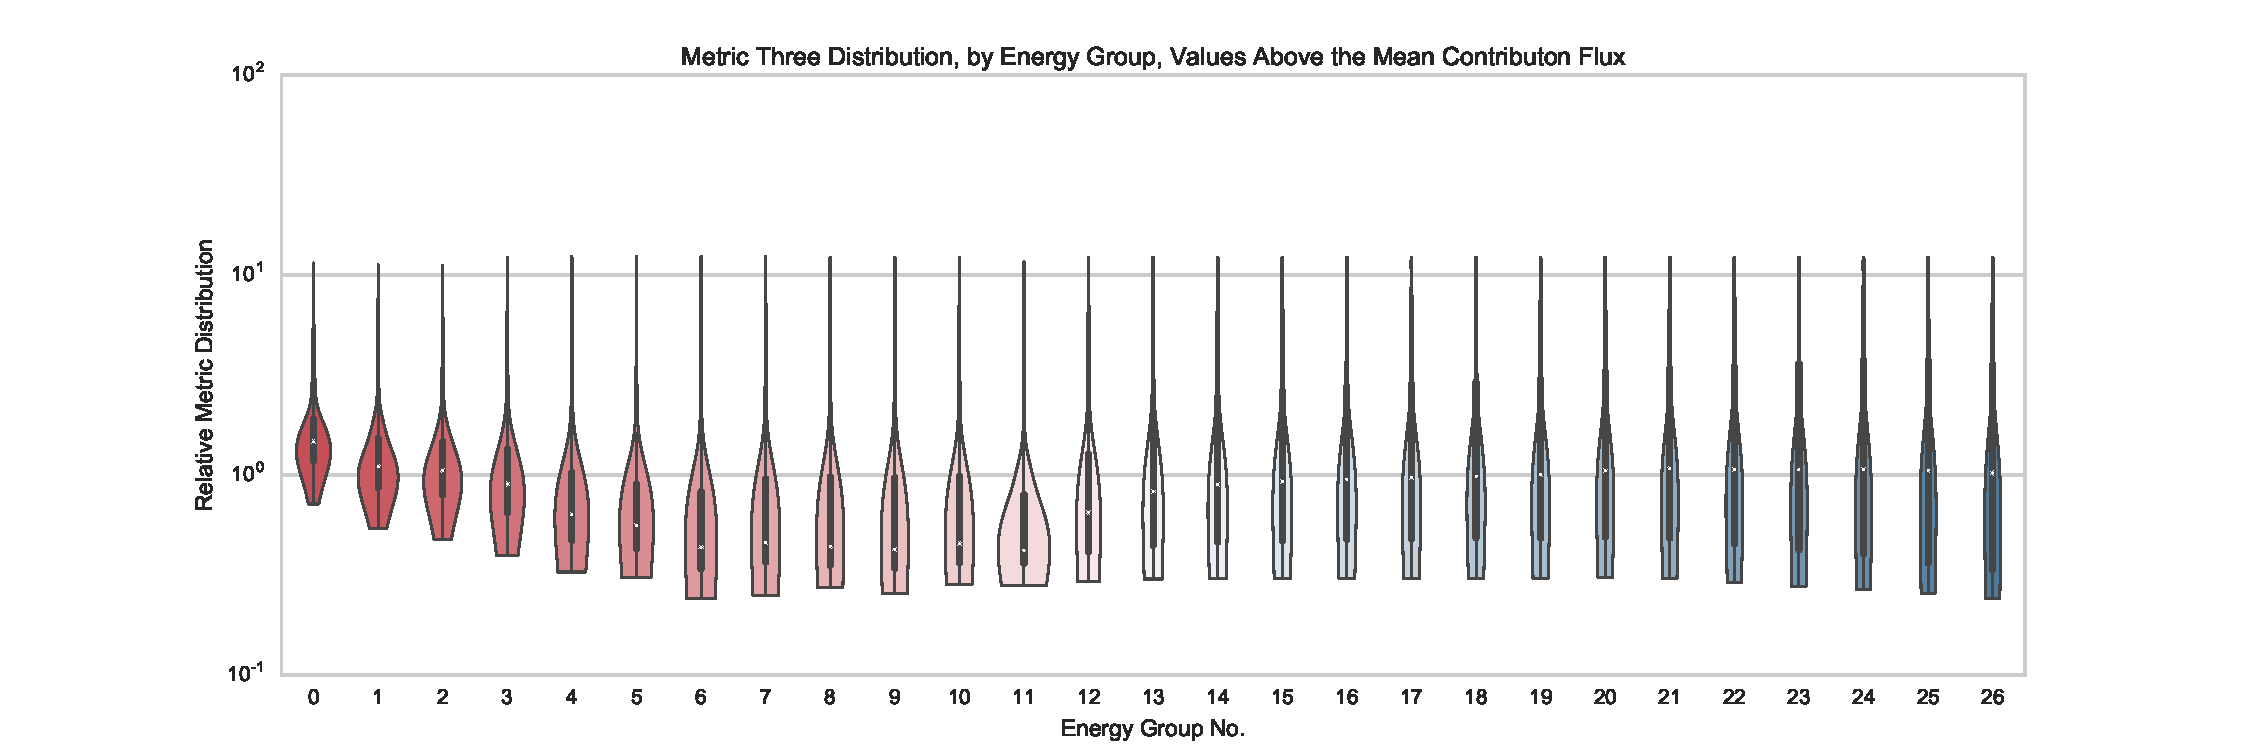
\includegraphics[width=\linewidth]{./chapters/characterization_probs/figures/char/maze2/metric_three_violin_mean.pdf}
    \caption{M$_{3}$ distribution for single turn labyrinth}
    \label{fig:maze2M3violins}
  \end{subfigure}
\end{figure}
\begin{figure}[htb!]\ContinuedFloat
  \centering
  \begin{subfigure}[t]{\textwidth}
    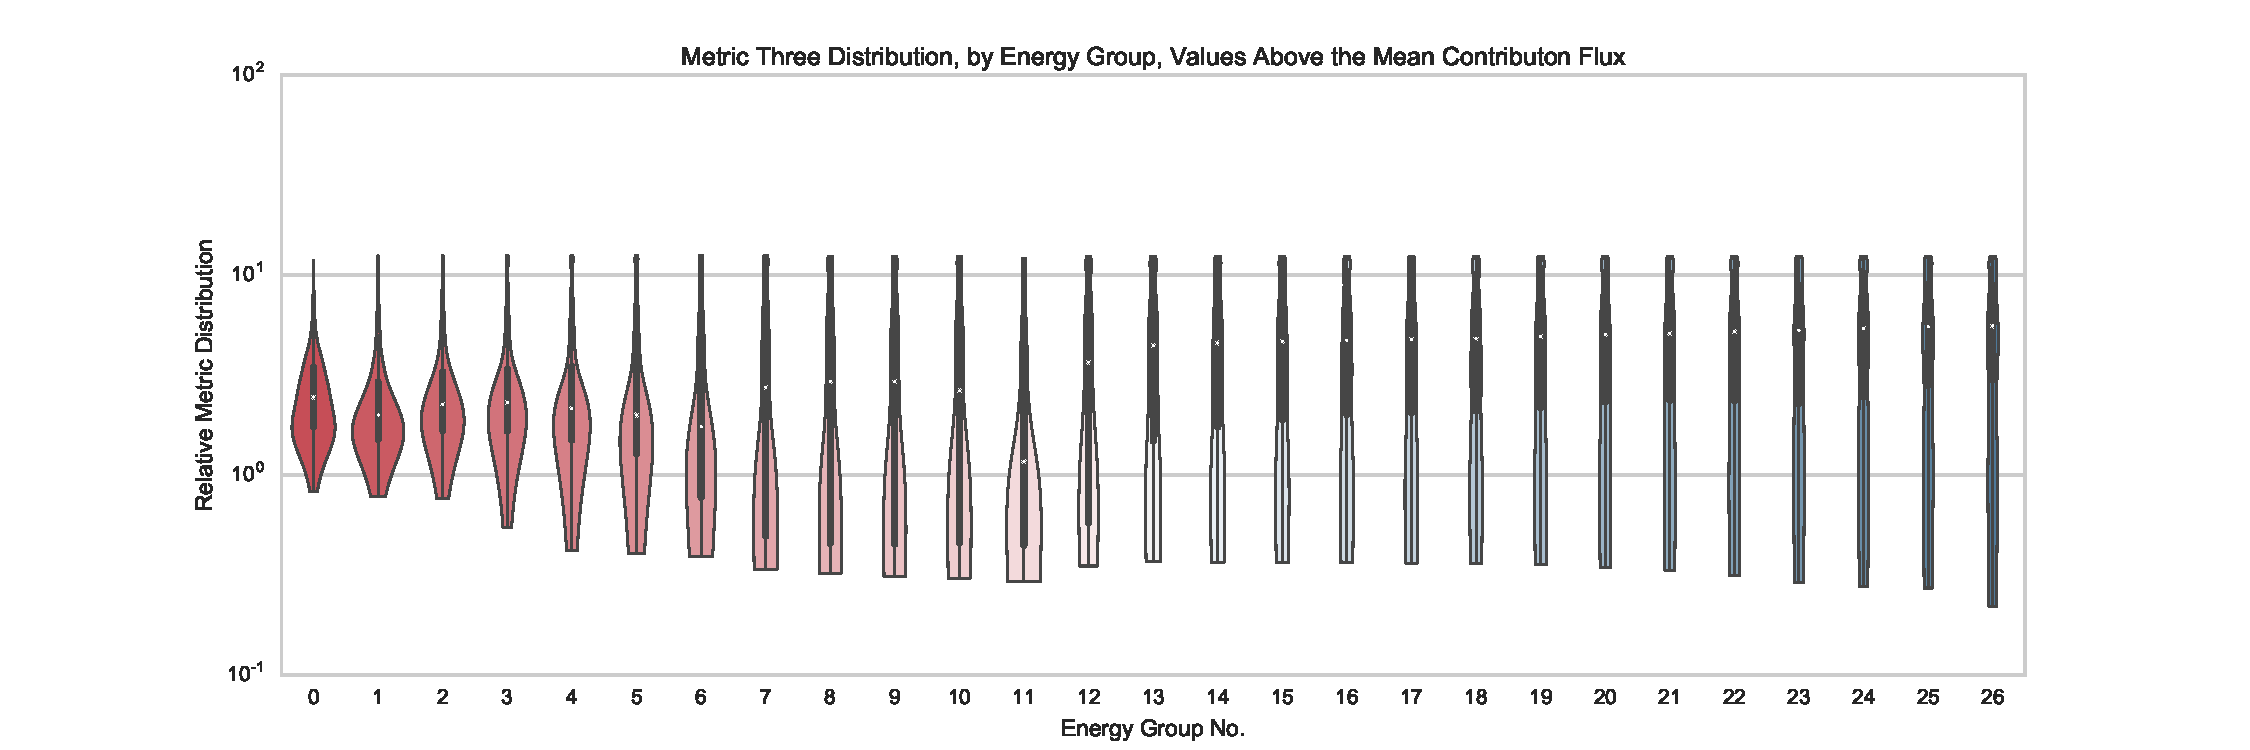
\includegraphics[width=\linewidth]{./chapters/characterization_probs/figures/char/maze1/metric_three_violin_mean.pdf}
    \caption{M$_3$ distribution for multi-turn labyrinth}
    \label{fig:maze1M3violins}
  \end{subfigure}
  \caption[Violin plots of M$_{3}$ distribution using values above the mean
  contributon flux for labyrinth problems.]
  {Violin plots of M$_{3}$ distribution using values above the mean
  contributon flux for labyrinth problems. Low energy group numbers correspond
  to high energies or fast particles, and are marked in red.}
  \label{fig:labyrinthviolins}
\end{figure}

The violin plots of the multi-turn labyrinth (Fig.~\ref{fig:maze1M3violins})
tend to span a larger range of values than the single turn. That is, the violins tend to be longer.
All of the violins in both plots have a bounding upper limit, meaning that in
every energy group there are some very anisotropic cells. 
% I don't htink that's what bounding upper limit means. 
Interestingly, it
appears that for the multi-turn labyrinth the distribution of anisotropies at
low energies has no distinctive bunching, as observed in the single-turn
labyrinth. This means that in important cells, there is an even distribution of
very anisotropic, slightly anisotropic, and isotropic cells.

\begin{figure}[htb!]
  \centering
  \begin{subfigure}[t]{\textwidth}
    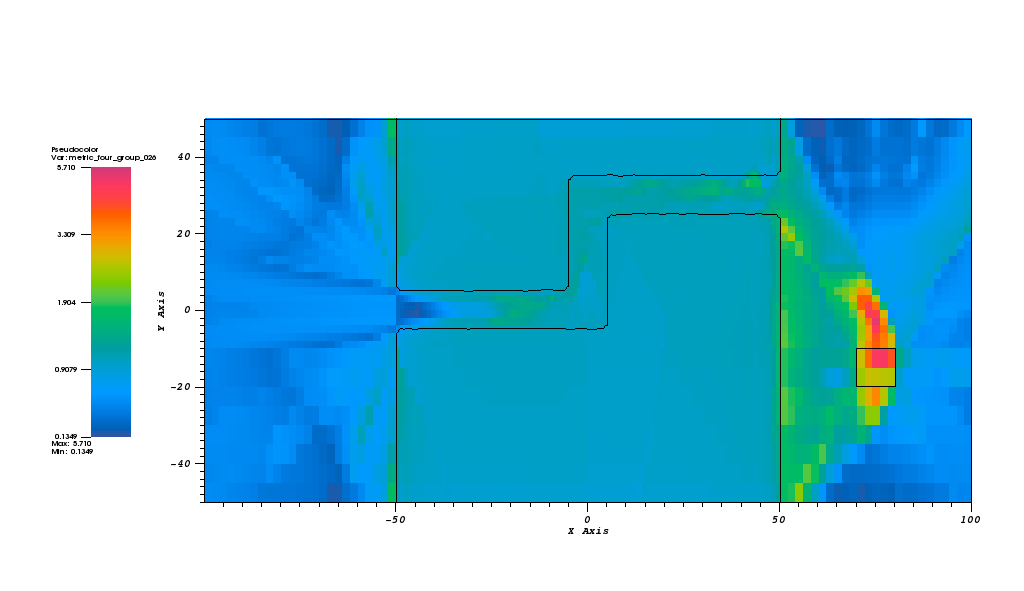
\includegraphics[width=0.9\linewidth]{./chapters/characterization_probs/figures/char/maze2/maze2M4G26.png}
    \caption{M$_4$ lowest energy group, single-turn
    labyrinth.}
    \label{fig:maze2M4}
  \end{subfigure}
\end{figure}
\begin{figure}[htb!]\ContinuedFloat
  \centering
  \begin{subfigure}[t]{\textwidth}
    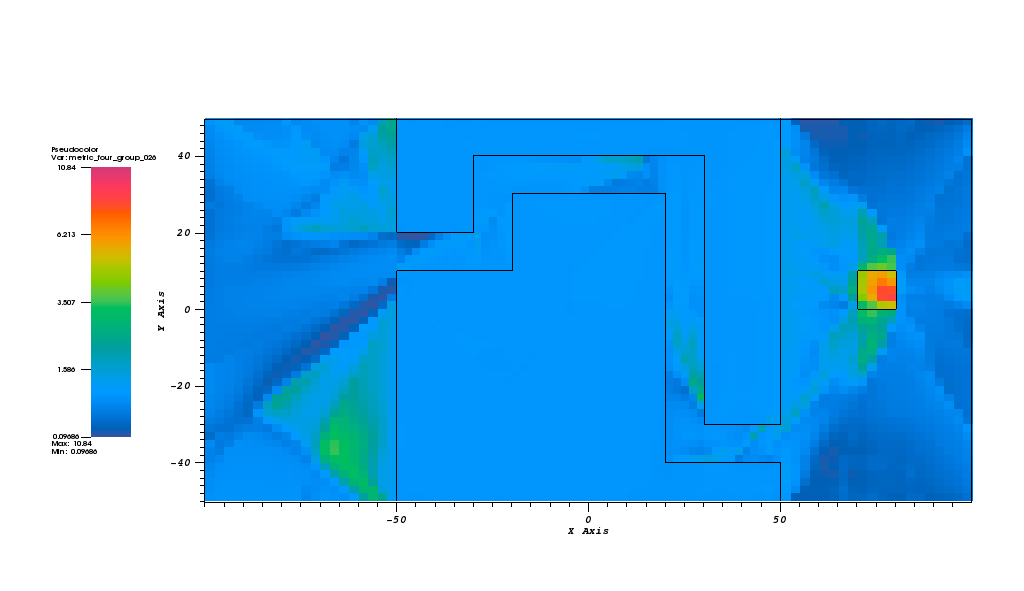
\includegraphics[width=0.9\linewidth]{./chapters/characterization_probs/figures/char/maze1/maze1M4G026.png}
    \caption{M$_4$ for lowest energy group, multi-turn labyrinth }
    \label{fig:maze1M4}
  \end{subfigure}
  \caption[M$_4$ distributions at problem midplane for labyrinth problems]{M$_4$
  distributions at problem midplane for labyrinth problems.}
  \label{fig:labyrinthM4}
\end{figure}

While the violin plots are useful in seeing
the overall distribution of metrics for the whole problem, it is also possible
to plot a given metric similarly to the flux maps. Figure
\ref{fig:labyrinthM4} shows the M$_4$ distribution for the single- and multiple-turn 
labyrinth problems. Recall that this metric is the ratio of the contributon
anisotropy to the standard adjoint anisotropy. Cells that have blue coloring
are those where the contributon max to average flux is lower than the adjoint.
As a result, the forward and adjoint fluxes do not synergistically combine in
angle. This
generally means this is a region of lower importance. Values of unity mean that
the contributon anisotropy is comparable to the adjoint anisotropy. In figure
\ref{fig:maze2M4}, it is clear that the concrete body of the maze is a region
where the anisotropies are similar, which makes sense.

Figure \ref{fig:maze2M4} shows that the region where the anisotropy of the
contributon flux differs the most from the adjoint flux is in the air region
near the detector, and also in the air regions of the maze. Specifically, the
anisotropy of the contributon flux is greater in the air region between the
detector and the labyrinth, and the anisotropy of the contributon flux is lower in
regions behind the detector. Conceptually, we expect this anisotropy behavior
in the region just past the detector, as the contributon flux will combine
positively if the forward and adjoint fluxes are traveling in opposite
directions, and will combine negatively if they are traveling in the same
direction. As a result, the anisotropy of the contributon flux behind the
detector will be minimized when compared to the original adjoint angular flux.

Figure \ref{fig:maze1M4} shows, like Figure \ref{fig:maze2M4}, the M$_4$
distribution at the problem midplane for the lowest energy group for
the multi-turn labyrinth. In this problem, we similarly see the strongest
anisotropy in the flux near the NaI detector. However, the range of values is
different. The concrete region of the maze still shows similar anisotropies
between the contributon and adjoint angular fluxes. The labyrinth edge next to the
NaI detector also has some fairly anisotropic regions, but overall the
anisotropies are less different in this problem than in the single-turn
labyrinth. As a result, CADIS-$\Omega$ does not have as much angular information
to capture, and its importance map is less effective. This was also illustrated
in the flux map comparison of Figure \ref{fig:maze1fluxmaps}.

Both figures have interesting secondary features in the anisotropy in the air
regions. These regions look similar to ray effects, but are not always reflected
in the flux maps themselves. The author is not sure how to explain these
effects, but they are worth future study.
% it might be a measure in the difference in ability to capture angular information as a result of angle discretization

It must be noted that, while
the trends in these violins are interesting, we must also be wary of comparing
the violins directly. The filtering algorithm used to pull values out is dependent only
on the contributon flux solution for that problem, so the average contributon
flux cutoff for the single-turn labyrinth and multiple-turn labyrinth are
different. Using a raw value from the violin plot in Figure
\ref{fig:maze1M3violins} and directly comparing it to one from Figure
\ref{fig:maze2M3violins} may be misleading. Instead, this analysis will focus on
the general behavior of the metrics in each problem, not specific metric values.

% same comment about broken up figures.
\begin{figure}[htb!]
  \centering
  \begin{subfigure}[t]{\textwidth}
    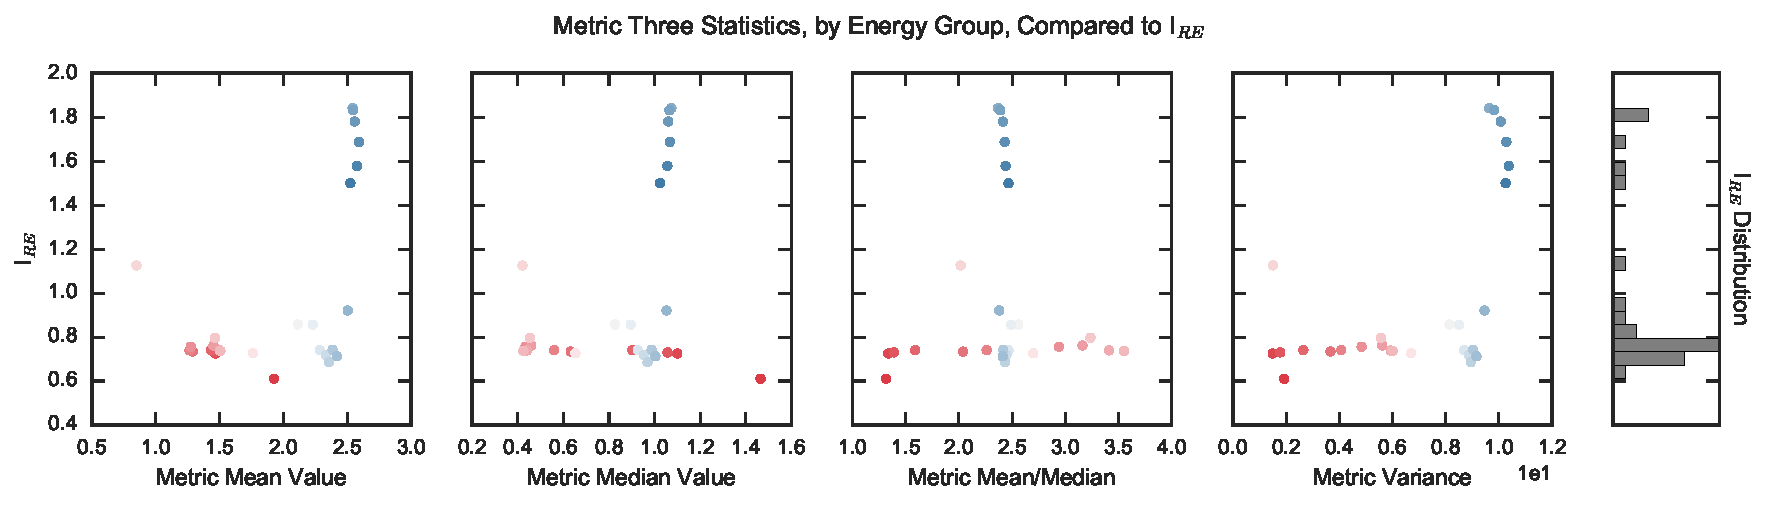
\includegraphics[width=\linewidth]{./chapters/characterization_probs/figures/char/maze2/metric_three_err_stats_mean.pdf}
    \caption{RE improvement factor as a function of M$_{3}$ statistics for single-turn labyrinth}
    \label{fig:maze2M3errs}
  \end{subfigure}
\end{figure}
\begin{figure}[htb!]\ContinuedFloat
  \centering
  \begin{subfigure}[t]{\textwidth}
    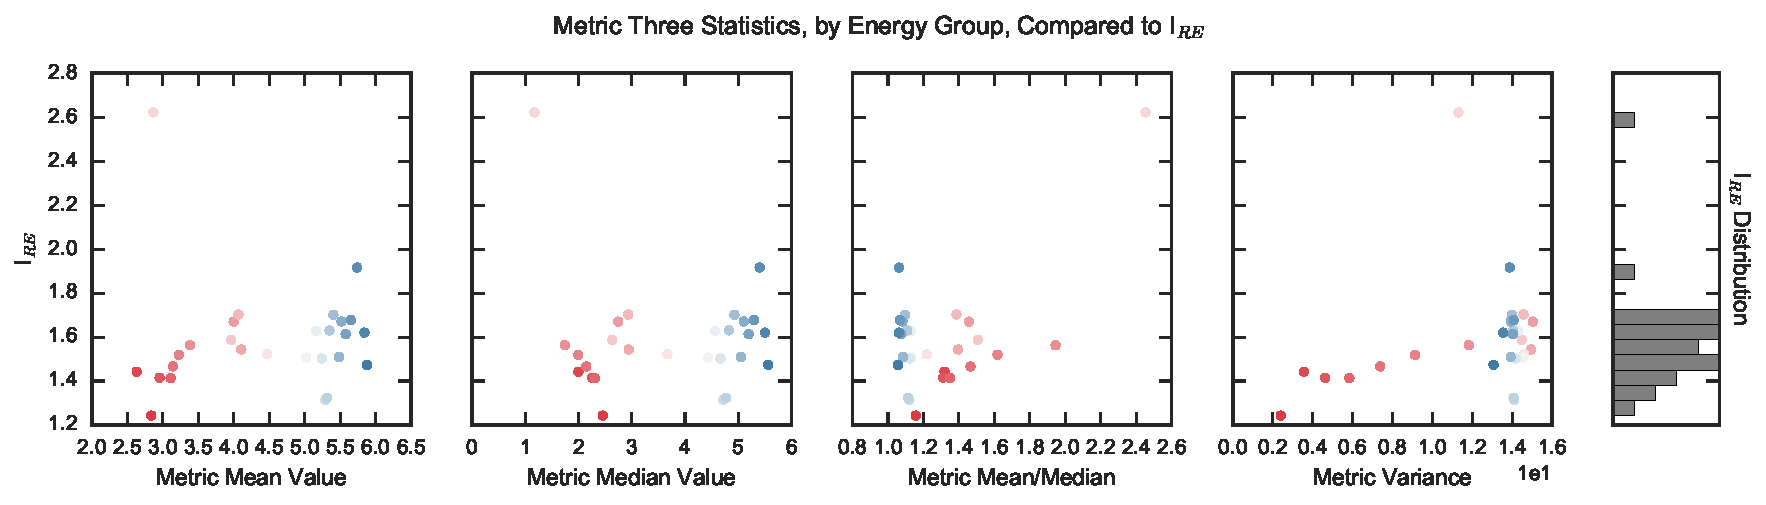
\includegraphics[width=\linewidth]{./chapters/characterization_probs/figures/char/maze1/metric_three_err_stats_mean.pdf}
    \caption{RE improvement factor as a function of M$_3$ statistics for multi-turn labyrinth}
    \label{fig:maze1M3errs}
  \end{subfigure}
  \caption[Relative error improvement factor as a function of M$_3$
  distribution statistics.]
  {Relative error improvement factor as a function of M$_3$
  distribution statistics. Metric distribution statistics are calculated using
  values of M$_3$ in cells with contributon flux values above the mean. Colors
  of data points correspond to the energy group to which they belong.}
  \label{fig:labyrinthIREs}
\end{figure}

% here is where you can put the explanation of these plots. 
Figures \ref{fig:labyrinthIREs} show the improvement factors of the relative
errors between CADIS-$\Omega$ and CADIS for the labyrinth problems. The x-axes
of the plots use the
distribution statistics from the violins in Figures \ref{fig:maze2M3violins} and
\ref{fig:maze1M3violins}, respectively. Recall that because I$_{RE}$ is the
ratio of the relative error between CADIS-$\Omega$ and CADIS--and we seek a low
relative error--that values of I$_{RE}$ below 1.0 indicate method improvement
for CADIS-$\Omega$.
% if you ever need to make the plots again, I'd add a line at 1 to help show it.

Looking at the differences between Figures \ref{fig:maze2M3errs} and
\ref{fig:maze1M3errs}, some interesting effects can be observed. Recall from the
relative error distribution plots for each problem (Figures \ref{fig:maze1error} and
\ref{fig:maze2error}) that CADIS-$\Omega$ had higher relative errors in all
energy bins than CADIS for the multi-turn labyrinth, and a higher relative
error in thermal energy groups in the single-turn labyrinth.
Figure
\ref{fig:maze2M3errs} shows the isolated grouping of poorer results for low
energy bins in the single-turn labyrinth. The rest of the values in this figure
all show improvement in the relative error, while the low-energy group show
better performance for CADIS. There is no distinct grouping in Figure
\ref{fig:maze1M3errs} because all of the CADIS-$\Omega$ relative errors are
higher than CADIS, so a distinct turnover in I$_{RE}$ does not occur.

There does not seem to be a tight
trend
observable for any measurement of the M$_3$ distribution and I$_{RE}$ in Figure
\ref{fig:maze2M3errs}, but the higher values of I$_{RE}$ generally occur in high
mean values of M$_3$ and higher variances of M$_3$. Figure \ref{fig:maze1M3errs}
also shows this trend in the metric mean and variance subplots, with a single
outlier in an intermediate energy group. It also appears that the spread of
I$_{RE}$ values does not change as a function of any of the metric values.

\begin{figure}[htb!]
  \centering
  \begin{subfigure}[t]{\textwidth}
    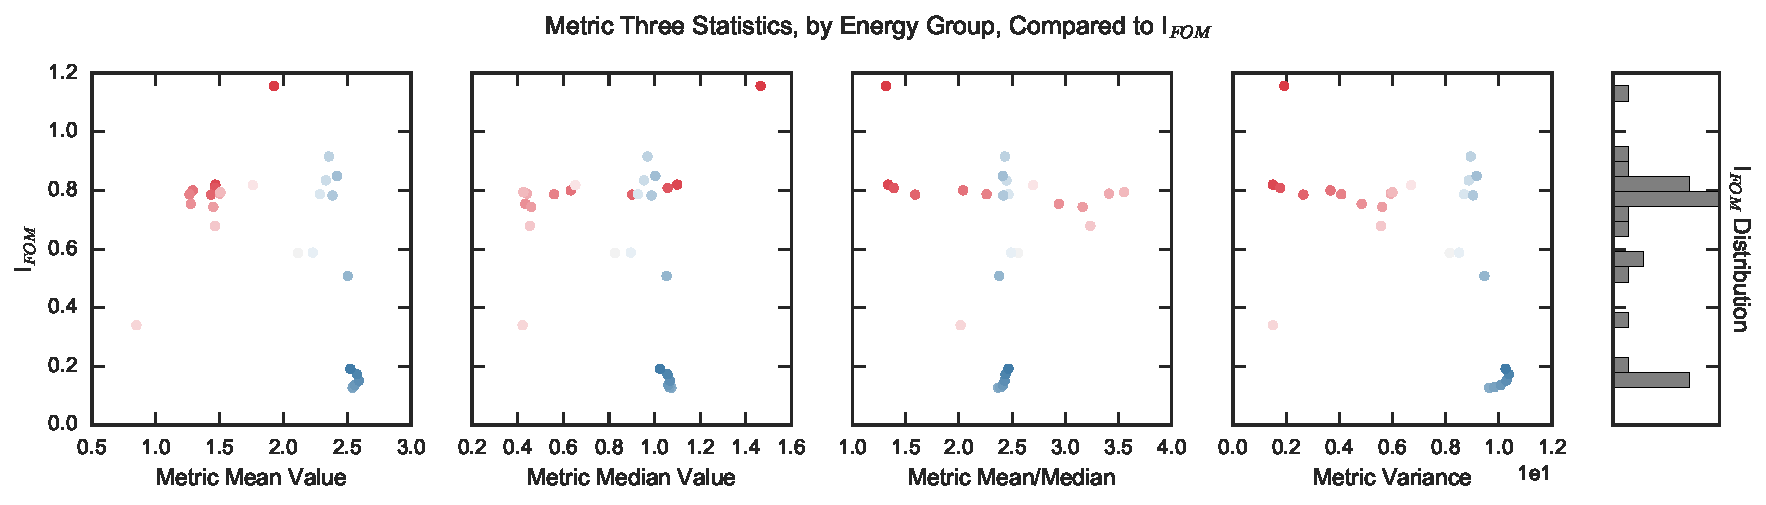
\includegraphics[width=\linewidth]{./chapters/characterization_probs/figures/char/maze2/metric_three_fom_stats_mean.pdf}
    \caption{FOM improvement factor as a function of M$_{3}$ statistics for single-turn labyrinth}
    \label{fig:maze2M3FOMs}
  \end{subfigure}
\end{figure}
\begin{figure}[htb!]\ContinuedFloat
  \centering
  \begin{subfigure}[t]{\textwidth}
    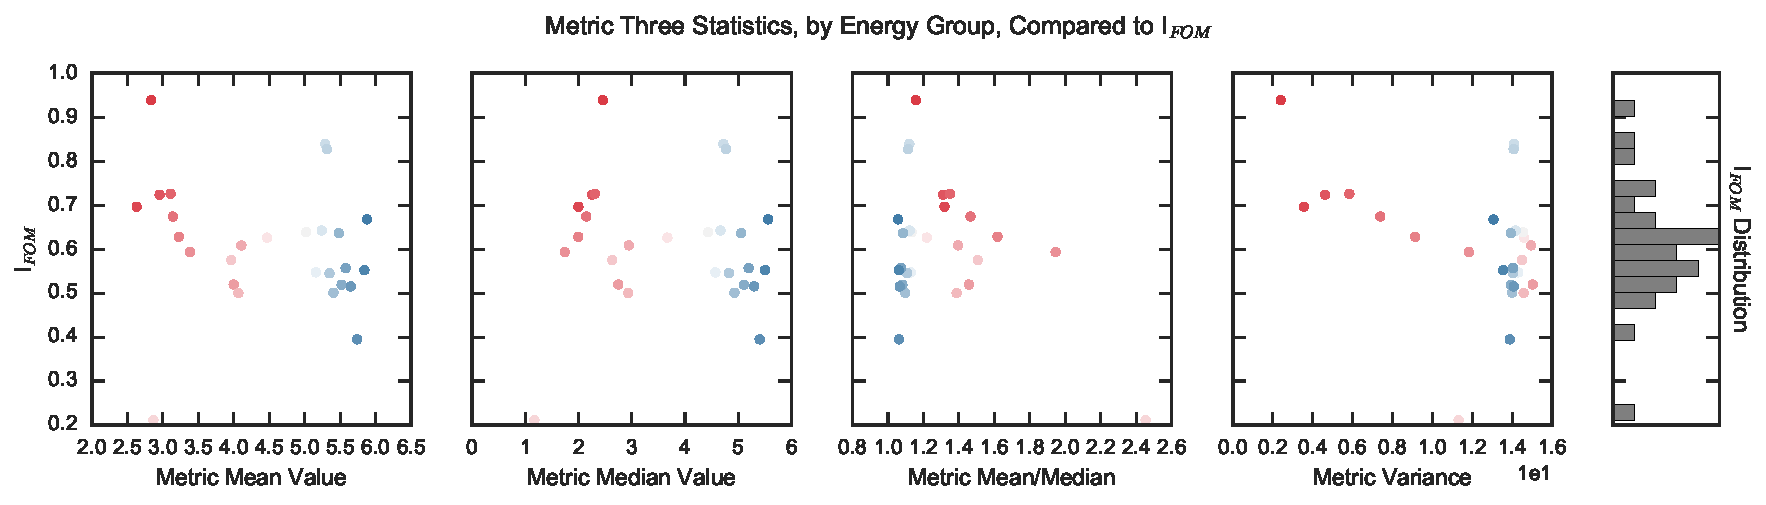
\includegraphics[width=\linewidth]{./chapters/characterization_probs/figures/char/maze1/metric_three_fom_stats_mean.pdf}
    \caption{FOM improvement factor as a function of M$_3$ statistics for multi-turn labyrinth}
    \label{fig:maze1M3FOMs}
  \end{subfigure}
  \caption[Figure of Merit improvement factor as a function of M$_3$
  distribution statistics.]
  {Figure of Merit improvement factor as a function of M$_3$
  distribution statistics. Metric distribution statistics are calculated using
  values of M$_3$ in cells with contributon flux values above the mean. Colors
  of data points correspond to the energy group to which they belong.}
  \label{fig:labyrinthIFOMs}
\end{figure}

Figure \ref{fig:labyrinthIFOMs} confirms what we've already observed in Figure
\ref{fig:labyrinthIREs}. In these figures, I$_{FOM}$ is plotted rather
than I$_{RE}$. If CADIS-$\Omega$ has better FOM performance than CADIS, the
resulting value of I$_{FOM}$ will be \textit{above} 1.0.

Many features from Figure \ref{fig:labyrinthIREs} are also present in Figure
\ref{fig:labyrinthIFOMs}. The distinct grouping of low-energy results for the
single-turn labyrinth are also observable in Fig.~\ref{fig:maze2M3FOMs}. The intermediate
energy outlier for the multiple turn labyrinth is located at the bottom of
all of the subplots in Figure \ref{fig:maze1M3FOMs}. By adjusting our results to
include timing, even less of a trend with metric distribution measurements is
seen in the improvement metric for the single turn labyrinth. However, for the
multi-turn labyrinth, it does appear that as the metric mean value increases,
I$_{FOM}$ decreases.

\subsection{Steel Beam}
\label{subsec:resultbeam}

The steel beam embedded in concrete FOM and timing
results are summarized in Tables
\ref{tab:steelbeamfoms} and \ref{tab:steelbeamtimes}. Figures
\ref{fig:steelbeamresult} and \ref{fig:steelbeamerror} show the results obtained
by the track length tally in CADIS, CADIS-$\Omega$ and the nonbiased analog
Monte Carlo.

\begin{table}[h!]
  \centering
  \begin{tabular}{lrrrrr}
\toprule
{} &    cadis &             & cadisangle &             & analog \\
{} &       MC & MC\_adjusted &         MC & MC\_adjusted &     MC \\
\midrule
tally avg   &      668 &         659 &      3e+03 &    2.96e+03 &   1.39 \\
max RE      &     3.74 &        3.69 &       6.79 &        6.71 & 0.0448 \\
min RE      & 1.43e+03 &    1.41e+03 &   1.33e+03 &    1.31e+03 &    -- \\
time (mins) &      414 &         420 &   2.09e+03 &    2.11e+03 &   22.3 \\
\bottomrule
\end{tabular}

  \caption[Figure of Merit comparison for steel bar embedded in concrete.]
  {Figure of Merit comparison for steel bar embedded in concrete. }
  \label{tab:steelbeamfoms}
\end{table}

\begin{table}[h!]
  \centering
  \begin{tabular}{llrrr}
\toprule
          &             &          CADIS & CADIS-$\Omega$ &         analog \\
        &              & \multicolumn{3}{c}{time (minutes)} \\
\midrule
MCNP time & total &         414.45 &        2086.60 &          22.33 \\
deterministic time & advantg\_time &           0.18 &           0.18 &            -- \\
          & denovo\_time &           5.69 &          25.64 &            -- \\
          & dispose\_time &           0.00 &           0.16 &            -- \\
          & omega\_time &           0.00 &           0.66 &            -- \\
          & total &           5.87 &          26.49 &            -- \\
wall time &              &         420.32 &        2113.09 &          22.33 \\
\bottomrule
\end{tabular}

  \caption[Detailed timing results for steel bar embedded in concrete.]
  {Detailed timing results for steel bar embedded in concrete.}
  \label{tab:steelbeamtimes}
\end{table}

Tables \ref{tab:steelbeamfoms} and
\ref{tab:steelbeamtimes} show that this problem is very difficult for
analog Monte Carlo and that CADIS-$\Omega$ generally performs better than CADIS.
In fact, CADIS-$\Omega$ has the best performance
in this problem of all of the characterization problems.

For both CADIS and CADIS-$\Omega$, this problem has a huge disparity in the FOMs
calculated with the maximum and minimum relative error. As a result, depending
on the convergence requirements that a user might require, the time to achieve
a desired solution could vary significantly in applications. However, both CADIS
and CADIS-$\Omega$ improve on the unbiased analog Monte Carlo's FOM by a factor
of $10^{2}$ or more.

CADIS-$\Omega$ outperforms CADIS for
the FOMS calculated with the tally average relative error and the tally maxmimum
relative error. This indicates that giving a limiting relative error to which
all energy bins must converge, CADIS-$\Omega$ will achieve it in $1/3$rd the time
that CADIS will. Further, CADIS-$\Omega$ has a better FOM than CADIS when the
deterministic runtimes are added. As shown in the timing table, the time to run
and generate the variance reduction parameters for CADIS-$\Omega$ will always be
longer than CADIS due to the addition of the forward transport run. The addition of
deterministic runtimes has the potential to lower the FOM of CADIS-$\Omega$ more than
that of CADIS, so CADIS-$\Omega$'s achievement of a FOM higher FOM with much
longer runtimes in both Monte Carlo and ADVANTG illustrates just how much lower
the relative error it achieves is. CADIS-$\Omega$ is very well-suited to a
problem with these conditions.

\begin{figure}[h!]
  \centering
  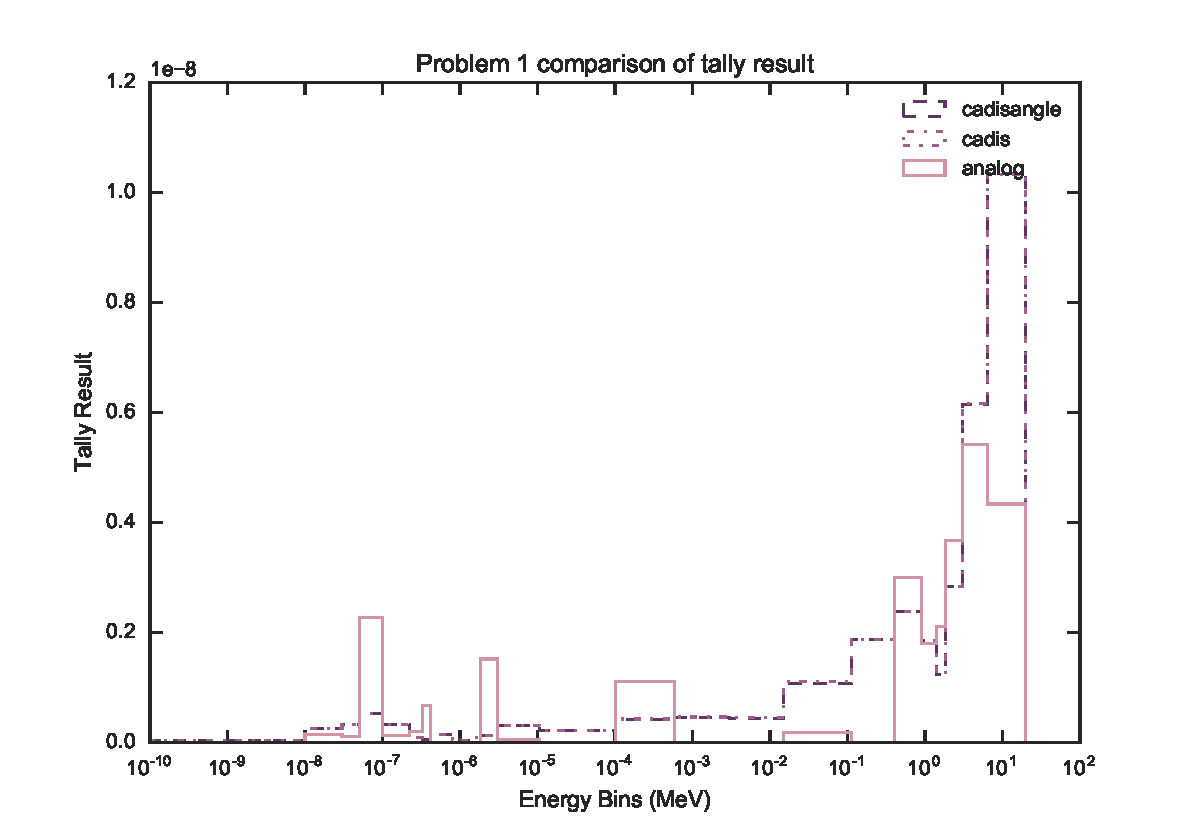
\includegraphics[height=10cm]{./chapters/characterization_probs/figures/char/prob_1/problem_1_tally_result_compare.pdf}
  \caption[Tally results comparison between methods for steel bar embedded in
  concrete.]
  {Tally results comparison between methods for steel bar embedded in concrete.}
  \label{fig:steelbeamresult}
\end{figure}

\begin{figure}[h!]
  \centering
  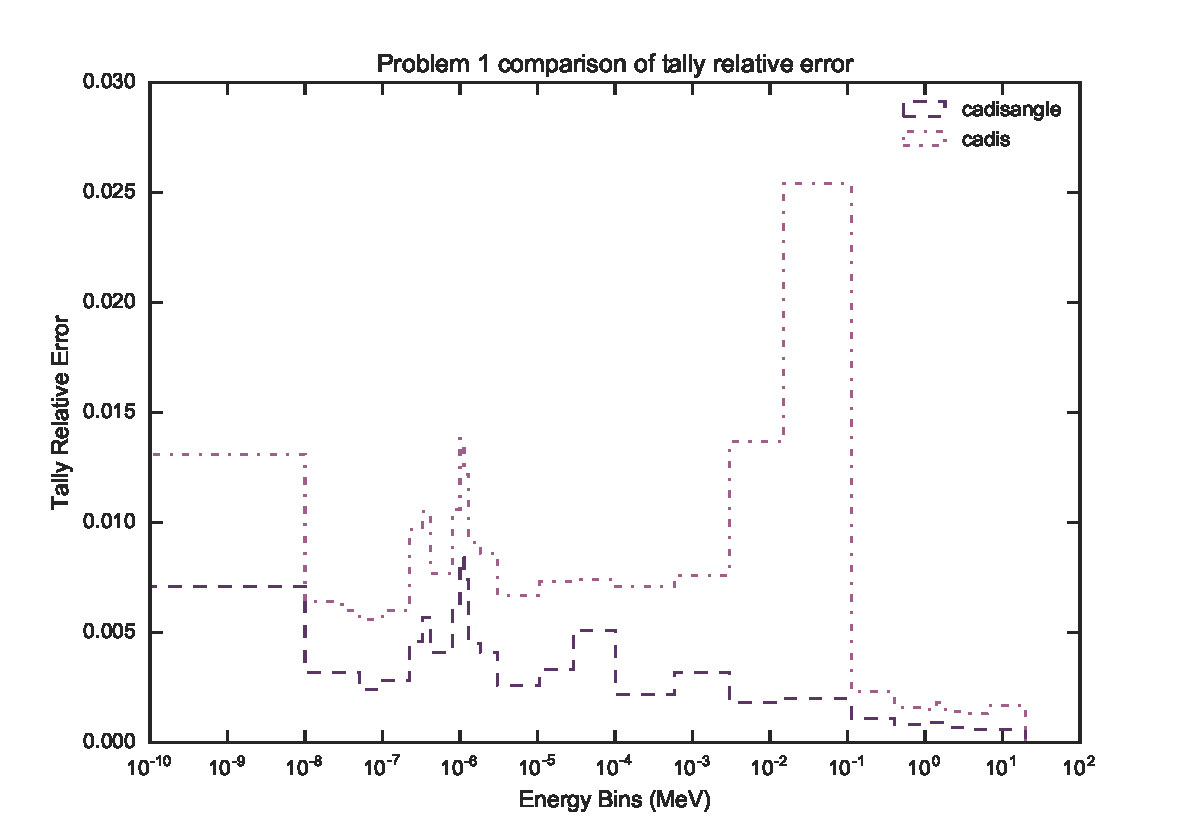
\includegraphics[height=10cm]{./chapters/characterization_probs/figures/char/prob_1/problem_1_tally_error_compare.pdf}
  \caption[Tally relative error comparison between methods for steel bar
  embedded in concrete.]
  {Tally relative error comparison between methods for steel bar embedded in
  concrete.}
  \label{fig:steelbeamerror}
\end{figure}

Figure \ref{fig:steelbeamresult} shows that CADIS and CADIS-$\Omega$ are in
agreement for the tally results in all energy bins. The nonbiased Monte Carlo
calculation differs from both of the hybrid methods. This supports what was
observed in the nonbiased analog FOM values of Table \ref{tab:steelbeamfoms}.
Figure
\ref{fig:steelbeamerror} shows that CADIS-$\Omega$ achieves a
consistently lower relative error than CADIS for all energy bins. For most
energy bins, CADIS-$\Omega$'s relative errors are shifted a consistent fraction
below CADIS'. In the energy regions between $10^{-4}$ and $10^{-1}$ MeV, this is
not the case. For these energy regions CADIS' relative errors spike while
CADIS-$\Omega$'s do not.

% [add anisotropy plots here]
%
% [describe why anisotropy might have happened in this region]
%
% [make visit plot of problematic energy group in adjoint flux and omega flux.
% compare and discuss differences.]

From the FOM results presented in Table \ref{tab:steelbeamfoms} and the tally
results and error in Figures \ref{fig:steelbeamresult} and
\ref{fig:steelbeamerror}, we can conclude that
CADIS-$\Omega$'s source biasing parameters consistently move more particles in
all tally energy bins more effectively than CADIS.
The importance map generated by CADIS-$\Omega$
better reflects the problem physics and more efficiently transports particles to
the desired tally location.

\subsubsection{Air Channel Variant}
\label{subsubsec:airbeam}

The characterization problems have been designed to induce anisotropy in
the flux. Most of these problems do so, in some part, by using air to induce
particle streaming. The steel beam in concrete problem requires that particles
interact with a high density material (either steel or concrete) before reaching
the detector to induce a response. These next two variant problems explore
whether the material choice of steel strongly affects the $\Omega$-method's
ability to generate variance reduction parameters. This first variant keeps the
geometric configuration of the steel beam problem the same, but the steel is
replaced with air. If the $\Omega$-methods are more sensitive to air, then this
change in the materials composition should affect the results.

\begin{table}[h!]
  \centering
  \begin{tabular}{lrrrrr}
\toprule
{} & cadis &             & cadisangle &             & analog \\
{} &    MC & MC\_adjusted &         MC & MC\_adjusted &     MC \\
\midrule
tally avg   &   432 &         390 &        396 &         364 &   5.63 \\
max RE      &  1.17 &        1.05 &      0.247 &       0.227 & 0.0467 \\
min RE      &   273 &         247 &        296 &         272 &    -- \\
time (mins) &  47.3 &        52.3 &        247 &         268 &   21.4 \\
\bottomrule
\end{tabular}

  \caption[Figure of Merit comparison for the air variant of the steel beam
  problem geometry.]
  {Figure of Merit comparison for air variant of the steel beam problem geometry. In this
  variant problem, the steel bar volume region is replaced with air to
exacerbate the suggested splitting issues encountered in other hybrid problems. }
  \label{tab:airbeamfoms}
\end{table}

\begin{table}[h!]
  \centering
  \begin{tabular}{llrrr}
\toprule
          &              &          cadis &     cadisangle &         analog \\
          &              & time (minutes) & time (minutes) & time (minutes) \\
\midrule
MCNP time & total &          47.29 &         246.83 &          21.42 \\
deterministic time & advantg\_time &           0.16 &           0.15 &            -- \\
          & denovo\_time &           4.90 &          20.50 &            -- \\
          & dispose\_time &           0.00 &           0.15 &            -- \\
          & omega\_time &           0.00 &           0.65 &            -- \\
          & total &           5.05 &          21.30 &            -- \\
wall time &              &          52.34 &         268.13 &          21.42 \\
\bottomrule
\end{tabular}

  \caption[Detailed timing results for steel beam geometry air variant.]
  {Detailed timing results for steel beam geometry air variant.}
  \label{tab:airbeamtimes}
\end{table}

Tables \ref{tab:airbeamfoms} and \ref{tab:airbeamtimes} summarize the FOM and timing
results for the air variant of the steel beam problem. Comparing the FOMs for
this variant and for the steel variant (Table \ref{tab:steelbeamfoms}), it is
clear that CADIS-$\Omega$ performs more poorly than CADIS with air.
Interestingly, CADIS-$\Omega$'s minimum relative error FOM is better than
CADIS', which is opposite to the results for the standard steel problem. For the
maximum relative error, CADIS-$\Omega$'s FOM is 1/5th that of CADIS'. However,
for this problem CADIS-$\Omega$'s runtime is almost five times that of CADIS.
Considering this time difference, it appears that CADIS-$\Omega$ requires far
more sampling with its importance map than CADIS. These sampling requirements
also exist with the original steel problem, but the importance map reduces the
tally variance enough to offset the time addition. This is not the case for the
air variant. From this, we can conclude that the addition of air into this
problem geometry reduces the sampling interaction points enough to negatively
affect the $\Omega$-method. Further, it lowers the FOMs achieved by both CADIS
and CADIS-$\Omega$ substantially that their improvement over the nonbiased
analog reduces almost an order of magnitude.

The runtimes in Table \ref{tab:airbeamtimes} are also worth comparing with the
original steel variant. In particular, the deterministic runtime in both of the
promblems is on the same order of magnitude. However, the Monte Carlo runtime is
far longer in the original steel version. The runtimes in the air variant are
generally much shorter for CADIS and CADIS-$\Omega$, but comparable for the
nonbiased analog. In this problem, the fraction of time spent in the
deterministic solve is much higher than in the steel version.

\subsubsection{Concrete Channel Variant}
\label{subsubsec:concretebeam}

In addition to the air variant of the steel beam geometry, we can see if having
non-preferential flowpaths might affect the $\Omega$-method's performance.
Recall that the $\Omega$-methods have been designed to incorporate angular
information into the importance map. If no preferential flowpaths exist through
the problem geometry, then the $\Omega$-importance map may have less of an
impact on improving the tally convergence. However, because the entire shield is
composed of concrete, then the distance to smapling location should still be
quite small as with the original steel version of the problem. As a result, there
should be some positive effects on the $\Omega$-methods due to sampling
interaction frequency. Tables \ref{tab:concretebeamfoms} and
\ref{tab:concretebeamtimes} show the FOM and timing results for this material
variant of the steel beam geometry.

\begin{table}[h!]
  \centering
  \begin{tabular}{lrrrrr}
\toprule
{} &    cadis &             & cadisangle &             & analog \\
{} &       MC & MC\_adjusted &         MC & MC\_adjusted &     MC \\
\midrule
tally avg   &  2.6e+03 &    2.55e+03 &   3.16e+03 &    3.13e+03 &   1.54 \\
max RE      &     14.5 &        14.2 &       9.48 &        9.39 & 0.0457 \\
min RE      & 1.54e+03 &    1.51e+03 &    1.4e+03 &    1.39e+03 &    -- \\
time (mins) &      385 &         393 &   1.98e+03 &       2e+03 &   21.9 \\
\bottomrule
\end{tabular}

  \caption[Figure of Merit comparison for concrete variant of steel bar geometry.]
  {Figure of Merit comparison for concrete variant of steel bar geometry. In this
  variant problem, the steel bar volume region is replaced with concrete to
  eliminate the preferential particle travel through the beam region.}
  \label{tab:concretebeamfoms}
\end{table}

\begin{table}[h!]
  \centering
  \begin{tabular}{llrrr}
\toprule
          &              &          cadis &     cadisangle &         analog \\
          &              & time (minutes) & time (minutes) & time (minutes) \\
\midrule
MCNP time & total &         385.11 &        1978.46 &          21.88 \\
deterministic time & advantg\_time &           0.23 &           0.15 &            -- \\
          & denovo\_time &           7.42 &          19.58 &            -- \\
          & dispose\_time &           0.00 &           0.09 &            -- \\
          & omega\_time &           0.00 &           0.56 &            -- \\
          & total &           7.65 &          20.29 &            -- \\
wall time &              &         392.76 &        1998.75 &          21.88 \\
\bottomrule
\end{tabular}

  \caption[Detailed timing results for concrete variant of steel bar.]
  {Detailed timing results for concrete variant of steel bar.}
  \label{tab:concretebeamtimes}
\end{table}

Tables \ref{tab:concretebeamfoms} and \ref{tab:concretebeamtimes} show the
results of the concrete variant of the steel beam problem. As with the original
steel and air versions described previously, the runtimes for CADIS-$\Omega$ are quite
long when compared to CADIS. In each variant, the runtimes are about five times
longer than those observed for CADIS. Similarly to the steel variant, in this
version CADIS-$\Omega$ achieves a superior FOM for the tally average FOM.
However, CADIS-$\Omega$'s FOMS for the maximum and minimum relative error FOMs
are both lower than CADIS'. Both CADIS and CADIS-$\Omega$ far outperform the
nonbiased analog Monte Carlo.

To compare the performance of each of the variants of this problem, let us first
compare the differences in the flux distributions for the $\Omega$ and CADIS
versions of the problem. Figure \ref{fig:steelbeamfluxes} shows the
adjoint and $\Omega$ fluxes for
the steel beam in concrete version of this geometry. It is clear from both of
these two figures that there is a preferential flowpath through the steel beam
for both the standard adjoint and for the $\Omega$-fluxes.

\begin{figure}[htb!]
  \centering
  \begin{subfigure}[t]{\textwidth}
    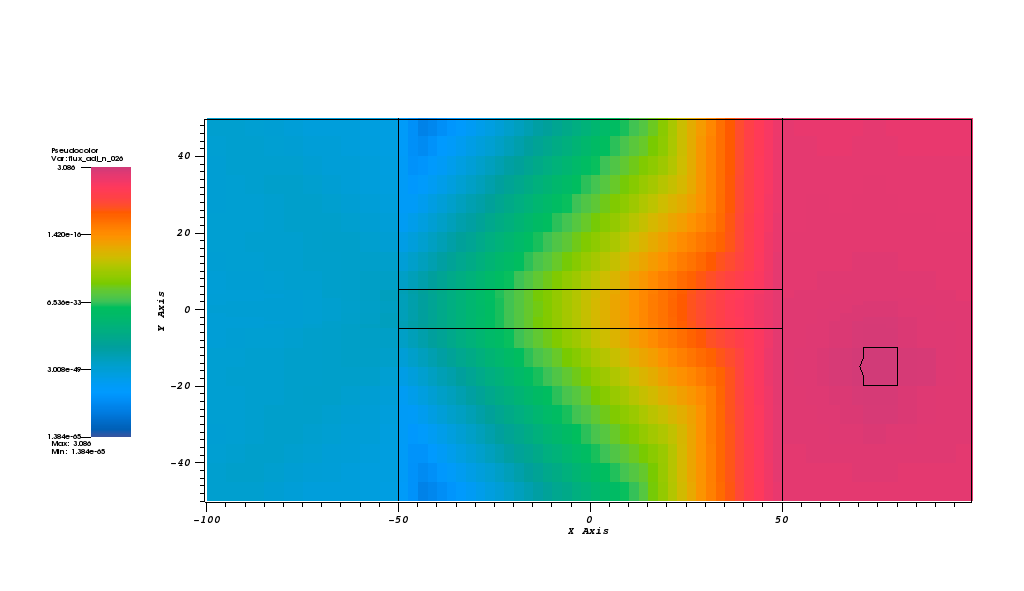
\includegraphics[width=0.9\linewidth]{./chapters/characterization_probs/figures/char/prob_1/prob1adjG26.png}
    \caption{Adjoint flux distribution, lowest energy group}
    \label{fig:steelbeamadj}
  \end{subfigure}
\end{figure}
\begin{figure}[htb!]\ContinuedFloat
  \centering
  \begin{subfigure}[t]{\textwidth}
    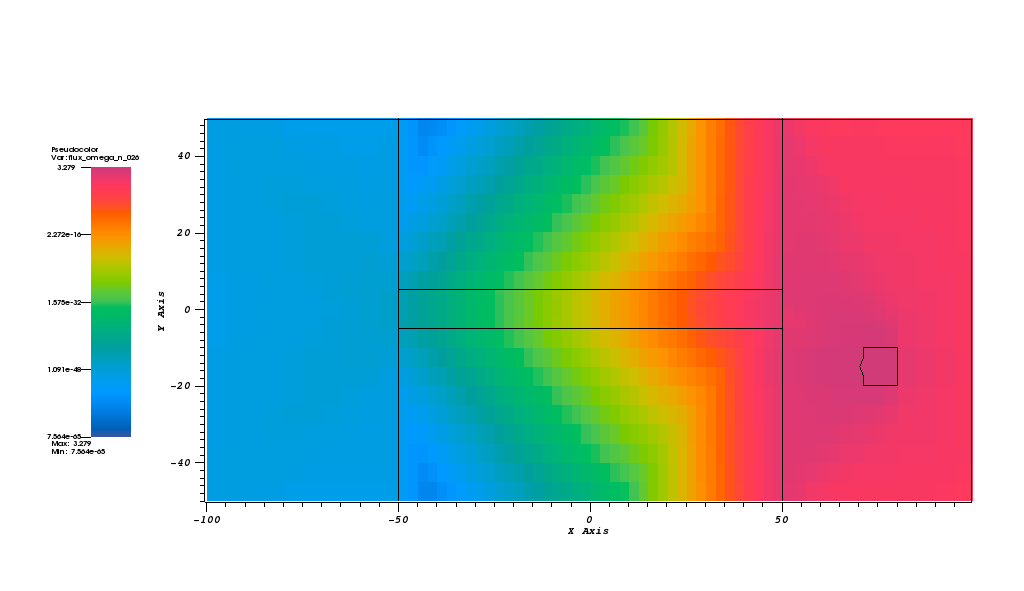
\includegraphics[width=0.9\linewidth]{./chapters/characterization_probs/figures/char/prob_1/prob1omegaG26.png}
    \caption{$\Omega$-flux distribution, lowest energy group}
    \label{fig:steelbeamomega}
  \end{subfigure}
  \caption[Flux maps for steel beam in concrete.]{Flux maps for steel beam in
  concrete. Fluxes shown are at problem midplane, and energy group 026. The
  colormap for each has been scaled to the data in the plane.}
  \label{fig:steelbeamfluxes}
\end{figure}

As with the multiple-turn
labyrinth, the flux maps are very similar between the adjoint and $\Omega$-flux
plots in this figure. Recall that M$_2$ is the ratio of the scalar $\Omega$-flux
to the scalar adjoint flux in each cell. Figure \ref{fig:M2beamplots} shows the
$M_2$ distributions for each of the material variants of the steel beam problem.
Figure \ref{fig:M2steel} contains the distribution of M$_2$ for the original
steel variant, Figure \ref{fig:M2air} is of the variant with air replacing the
steel, and Figure \ref{fig:M2concrete}. Note that Figure \ref{fig:M2air} has the
colormap scaled to a log scale, while the other two figures do not. This is
because the range is much larger in this figure, and a linear scale obscures the
data.

\begin{figure}[htb!]
  \centering
  \begin{subfigure}[t]{\textwidth}
    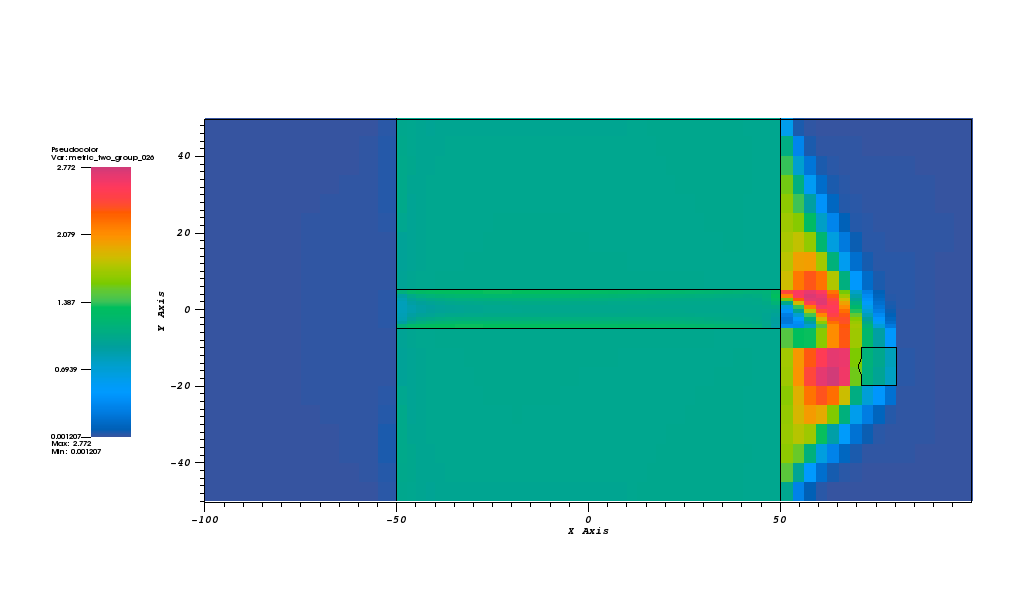
\includegraphics[width=0.9\linewidth]{./chapters/characterization_probs/figures/char/prob_1/prob1M2G26.png}
    \caption{M$_2$ distribution for steel beam in concrete.}
    \label{fig:M2steel}
  \end{subfigure}
\end{figure}
\begin{figure}[htb!]\ContinuedFloat
  \centering
  \begin{subfigure}[t]{\textwidth}
    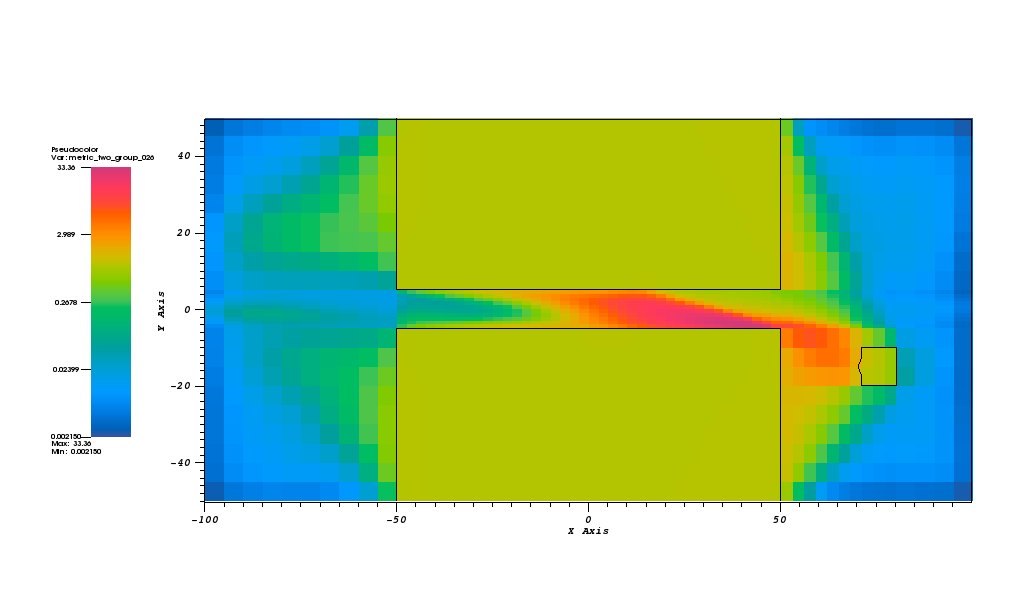
\includegraphics[width=0.9\linewidth]{./chapters/characterization_probs/figures/char/prob1v1/prob1v1M2G026log.png}
    \caption{M$_2$ distribution for steel beam in concrete, air variant.}
    \label{fig:M2air}
  \end{subfigure}
\end{figure}
\begin{figure}[htb!]\ContinuedFloat
  \centering
  \begin{subfigure}[t]{\textwidth}
    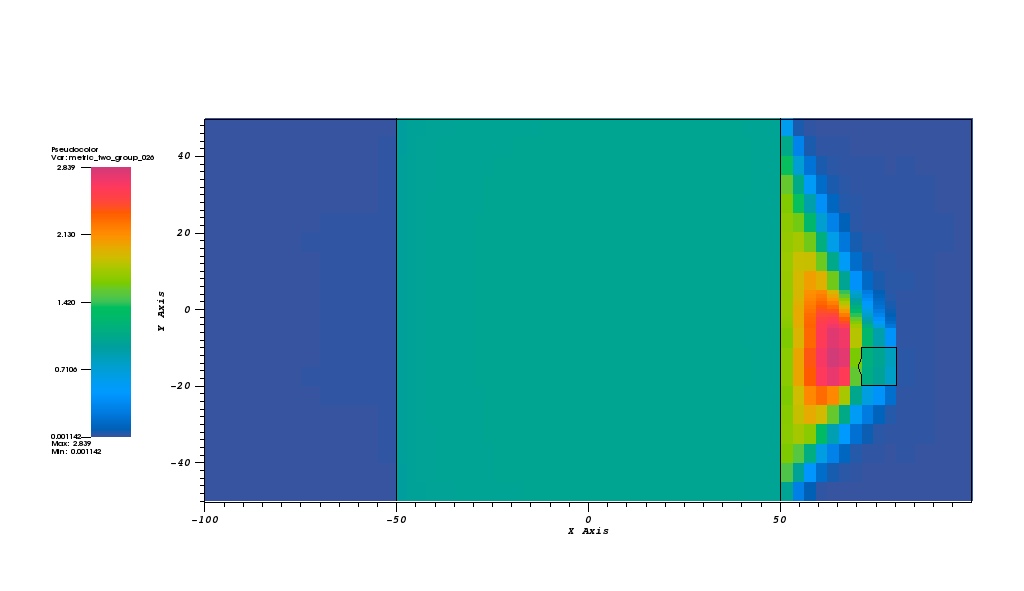
\includegraphics[width=0.9\linewidth]{./chapters/characterization_probs/figures/char/prob1v2/prob1v2M2G26.png}
    \caption{M$_2$ distribution for steel beam in concrete, concrete variant.}
    \label{fig:M2concrete}
  \end{subfigure}
  \caption[M$_2$ distribution plots for material variants of steel beam in
  concrete.]{M$_2$ distribution plots for material variants of steel beam in
  concrete. Distribution shown is for lowest energy group. Scales adjusted to
  match dataset of each figure.}
  \label{fig:M2beamplots}
\end{figure}

By comparing the ratio of the $\Omega$- to adjoint-fluxes in each of the figures
in \ref{fig:M2beamplots}, the effect that material choice has on changing the
$\Omega$-flux becomes more apparent. First, all three plots show a constant
value of M$_2$ within the concrete shield itself. As a result, we can conclude
that materials in which the particles have a small mean free path of travel, the
flux isotropy is fairly constant and does not differ between the $\Omega$- and
adjoint fluxes. Next, having a preferential flowpath through the shield does
change the resultant $\Omega$-flux. Depending on material, the flux may be very
different (as with the air in Figure \ref{fig:M2air}) or fairly similar (as with
the flux ratio in the steel in Figure \ref{fig:M2steel}). All three problems
show a very different distribution of fluxes near the adjoint source. This is
the case with both of the labyrinth variants previously discussed.

\begin{figure}[htb!]
  \centering
  \begin{subfigure}[t]{\textwidth}
    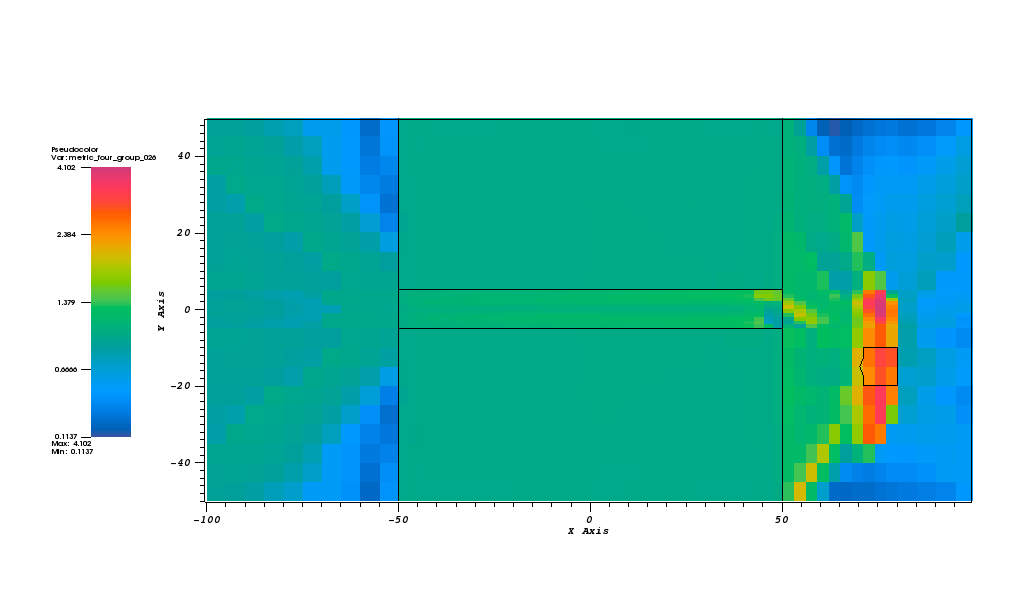
\includegraphics[width=0.9\linewidth]{./chapters/characterization_probs/figures/char/prob_1/prob1M4G26.png}
    \caption{M$_4$ distribution for steel beam in concrete.}
    \label{fig:M4steel}
  \end{subfigure}
\end{figure}
\begin{figure}[htb!]\ContinuedFloat
  \centering
  \begin{subfigure}[t]{\textwidth}
    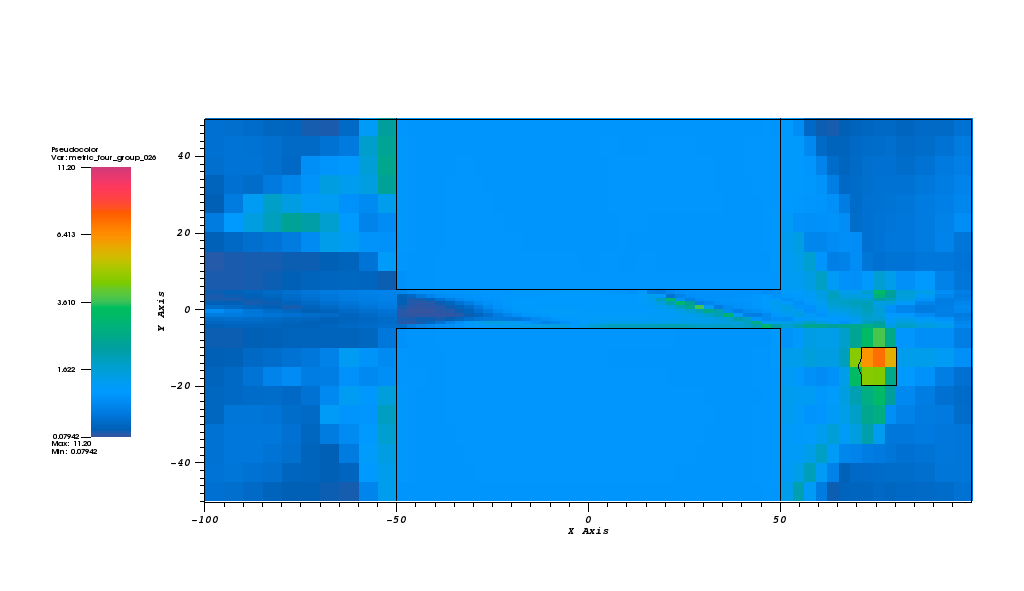
\includegraphics[width=0.9\linewidth]{./chapters/characterization_probs/figures/char/prob1v1/prob1v1M4G26.png}
    \caption{M$_4$ distribution for steel beam in concrete, air variant.}
    \label{fig:M4air}
  \end{subfigure}
\end{figure}
\begin{figure}[htb!]\ContinuedFloat
  \centering
  \begin{subfigure}[t]{\textwidth}
    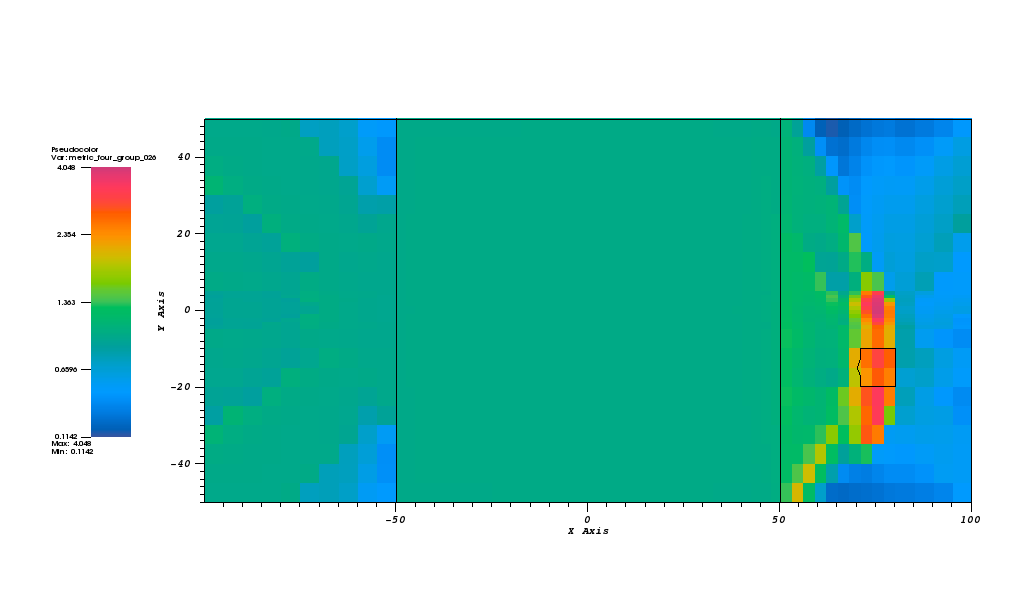
\includegraphics[width=0.9\linewidth]{./chapters/characterization_probs/figures/char/prob1v2/prob1v2M4G26.png}
    \caption{M$_4$ distribution for steel beam in concrete, concrete variant.}
    \label{fig:M4concrete}
  \end{subfigure}
  \caption[M$_4$ distribution plots for material variants of steel beam in
  concrete.]{M$_4$ distribution plots for material variants of steel beam in
  concrete. Distribution shown is for lowest energy group. Scales adjusted to
  match dataset of each figure.}
  \label{fig:M4beamplots}
\end{figure}

The subfigures of Figure \ref{fig:M4beamplots} complement those presented in
Figure \ref{fig:M2beamplots}. As with Figure \ref{fig:M2beamplots}, the
subfigures here are normalized by the adjoint problem. Rather than comparing the
adjoint scalar fluxes, here the contributon anisotropy in each
cell is compared to the adjoint. Similar features can be observed between the
subfigures in \ref{fig:M4beamplots} and their counterparts in
\ref{fig:M2beamplots}. For exmaple, the anisotropies in the cells in the shield
are the same as the adjoint. As a result, we see little- to no- difference
between the $\Omega$-method aniosotropy or the standard adjoint anisotropy.
Figure \ref{fig:M4air} shows some interesting streaming effects on the
anisotropy in the air channel within the shield. In particular, the contributon
anisotropy is larger for the majority of the air channel than the adjoint
anisotropy. There is an exception to this observation at the M$_4$ values marked
with dark blue in the air channel.

All three subfigures in \ref{fig:M4beamplots} show that there exist differences
in the anisotropy near the adjoint source and near the forward source in all
material variants of this problem. Unlike the subfigures of
\ref{fig:M2beamplots}, the anisotropies extend all the way to the problem
boundaries in the air regions of the problem. However,
the anisotropy in the area of each
problem near the detector is generally larger than the anisotropy in the area
neaer the forward source.

With an intuition of how the $\Omega$ and adjoint-scalar fluxes differ both on
the cell-scale, and how their anisotropies differ on the cell scale, we can
now look at the effectiveness of each at predicting the $\Omega$-method's
success (or lack thereof). Recall that Figures \ref{fig:M2beamplots} and
\ref{fig:M4beamplots} show the anisotropy distributions for the lowest energy
group. On the next several figures, the data illustrated by these figures will
correspond with the
darkest blue violin and the darkest blue scatterplot data point, respectively.
The next several figures attempt to collapse the substantial quantity of data
available in Figures \ref{fig:M2beamplots} and \ref{fig:M4beamplots} to
values with which we can correlate with $\Omega$- relative error or FOM
improvement.

\begin{figure}[htb!]
  \centering
  \begin{subfigure}[t]{\textwidth}
    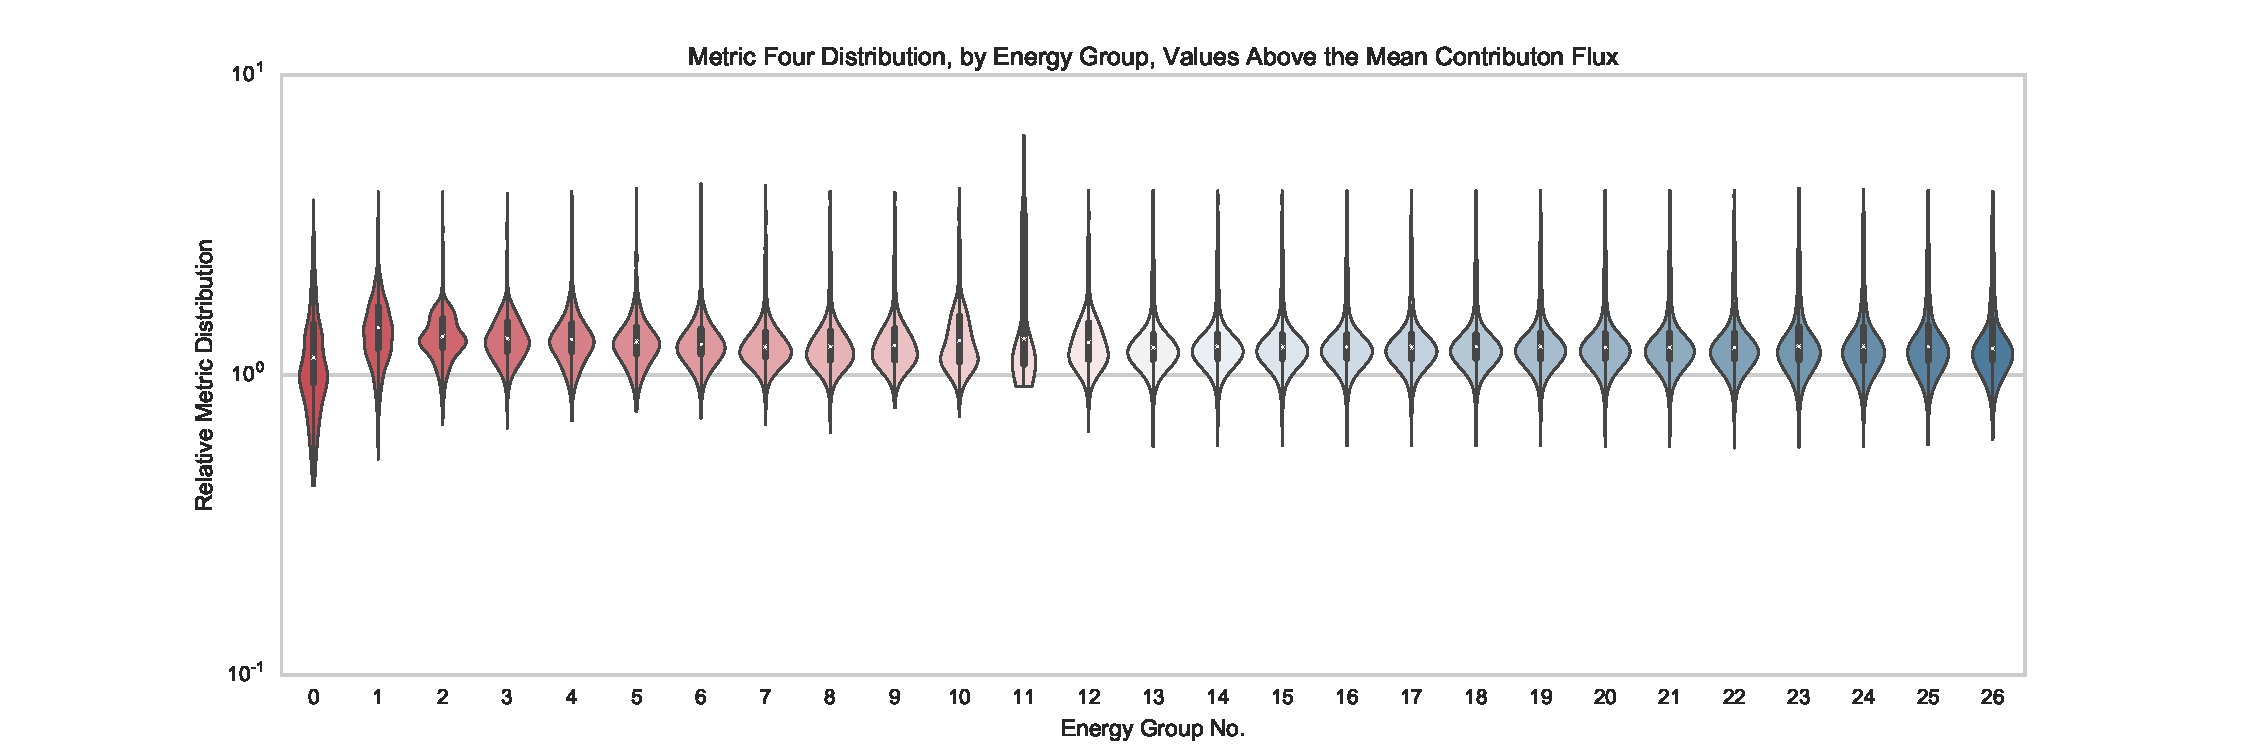
\includegraphics[width=\linewidth]{./chapters/characterization_probs/figures/char/prob_1/metric_four_violin_mean.pdf}
    \caption{M$_4$ distribution for steel beam geometry}
    \label{fig:beamsteelviolins}
  \end{subfigure}
\end{figure}
\begin{figure}[htb!]\ContinuedFloat
  \centering
  \begin{subfigure}[t]{\textwidth}
    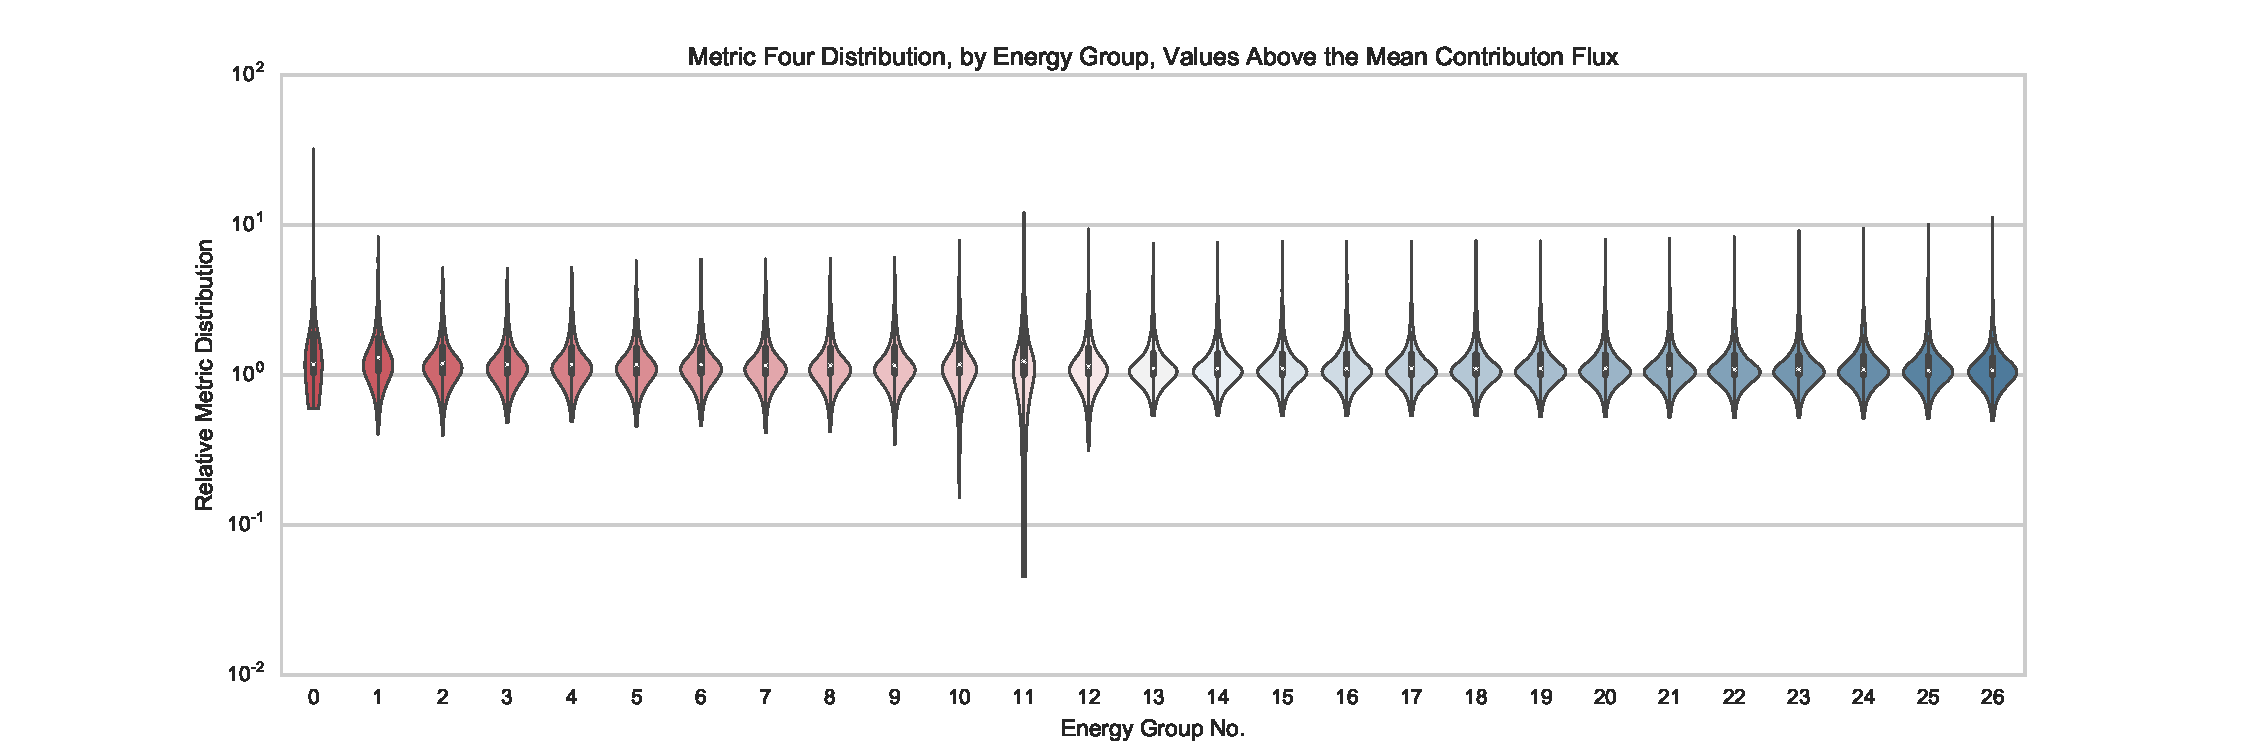
\includegraphics[width=\linewidth]{./chapters/characterization_probs/figures/char/prob1v1/metric_four_violin_mean.pdf}
    \caption{M$_4$ distribution for air beam geometry}
    \label{fig:beamairviolins}
  \end{subfigure}
\end{figure}
\begin{figure}[htb!]\ContinuedFloat
  \centering
  \begin{subfigure}[t]{\textwidth}
    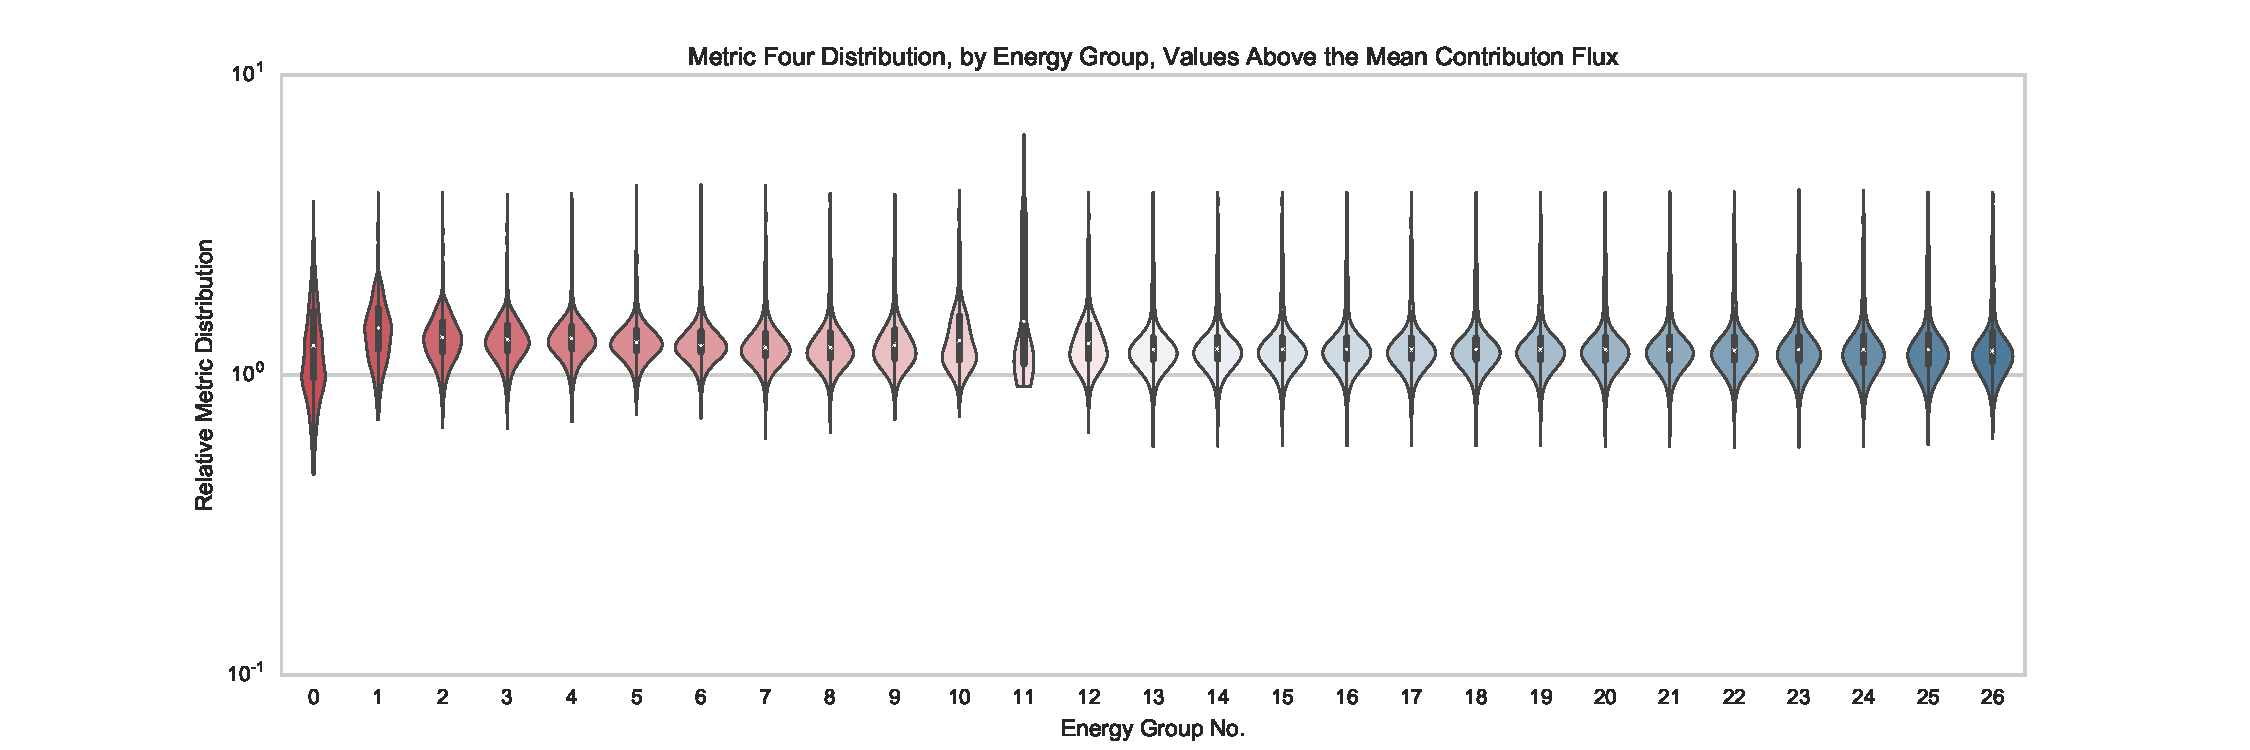
\includegraphics[width=\linewidth]{./chapters/characterization_probs/figures/char/prob1v2/metric_four_violin_mean.pdf}
    \caption{M$_4$ distribution for concrete beam geometry}
    \label{fig:beamconcreteviolins}
  \end{subfigure}
  \caption[Distribution plots of M$_4$ for the steel beam problem geometry
  material variants.]{Distribution plots of M$_4$ for the steel beam problem
  geometry material variants. Distributions have been filtered from cells that
  are in bins above the contributon average flux in each problem. Coloring
corresponds to energy group, red indicates a higher energy group and blue a
lower energy group. }
  \label{fig:beamviolins}
\end{figure}

The beam problem material variants provide a very interesting opportunity to see
the effect of material properties on I$_{RE}$ and on the anisotropy metric
distributions. Based on observations, the distributions for M$_4$ will be shown
for these problem variants in \ref{fig:beamviolins} and \ref{fig:beamIREs}.
Figure \ref{fig:beamsteelviolins} shows the M$_4$ distribution for each energy
group as a violin plot for the original steel version of the problem.
Figures \ref{fig:beamairviolins} and \ref{fig:beamconcreteviolins} show the air
and concrete variants of the problem, respectively. Note the similarity between
the metric distributions for the steel and concrete variants of the problem
(Figs. \ref{fig:beamsteelviolins} and \ref{fig:beamconcreteviolins}). The metric
distributions have similar ranges, similar distributions, and similar mean
values. The only energy groups where there are noticeable differences are in the
highest energy groups, where the local minimum values differ, and in energy
group three, where the distribution between the two problems differs.

Compare
what was observed in the concrete and steel variations of the problem
to Figure \ref{fig:beamairviolins}, which contains the M$_4$ distributions
for air. The range in values for each of these violins is much larger than
either \ref{fig:beamsteelviolins} or \ref{fig:beamconcreteviolins}. Energy group
11 does not bottom out as it does in the previous two problems. The fastest
energy group is strongly peaked upwards, as are many low energy groups. While
the distribution of each of the metrics for this problem are much broader, the
main body of the distributions are centered around lower values than either
\ref{fig:beamsteelviolins} and \ref{fig:beamconcreteviolins}.

The differences in the violin plots are purely due to differences in the
sampling physics of the problem. Despite different materials in the concrete and
steel variants of the problem,
\ref{fig:beamconcreteviolins} and \ref{fig:beamsteelviolins} have similar violin
distributions. This tells us that while the overall energy spectrum of the
problem may be different, the distribution of anisotropy within the problem may
be more dependent on how likely particles are to collide. That is, because both
steel and concrete have higher interaction probabilities than air, their
anisotropy distributions will be closer to each other than air.

Because the problem geometries and mesh sizes are identical between each of
these problems, it is likely that the selection of values is at similar
locations in each of the problems. However, because the filter matrix described
in Section \ref{subsec:resultsintro} is based on the contributon flux, which is
problem specific, these will still differ between problems. Further, the number
of cells selected from each energy group will differ between problems.


\begin{figure}[htb!]
  \centering
  \begin{subfigure}[t]{\textwidth}
    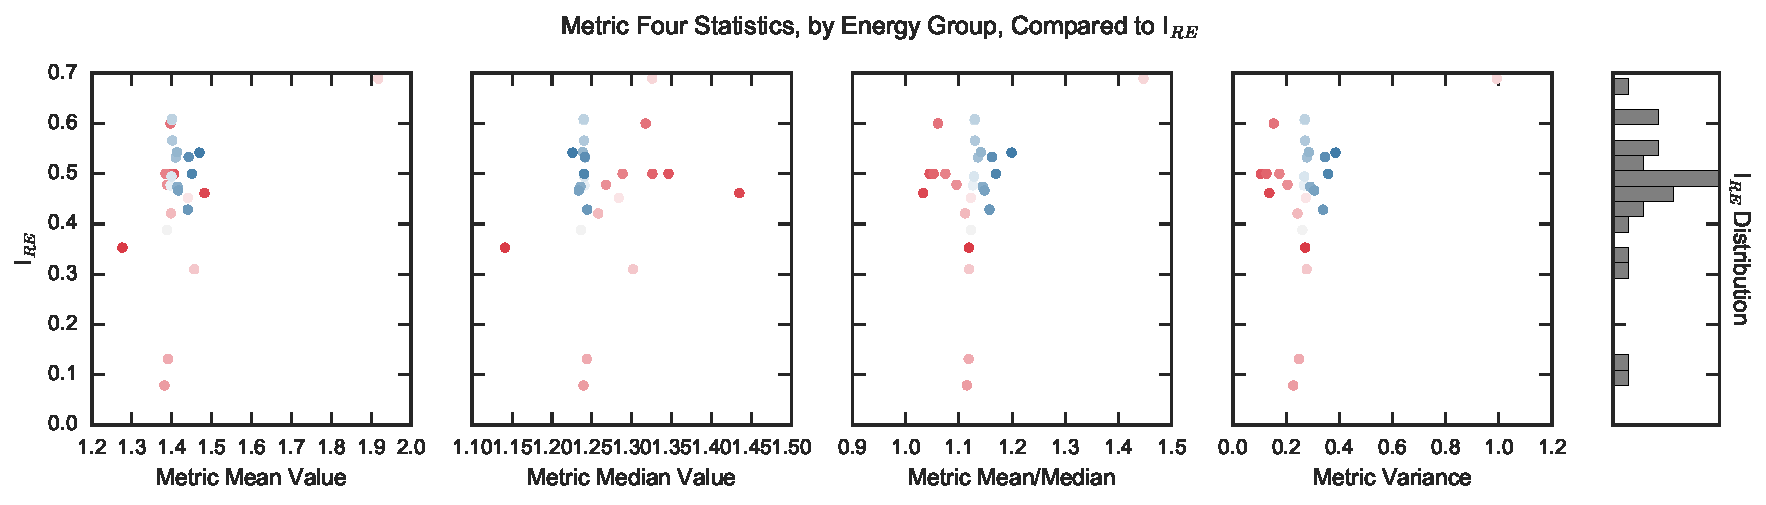
\includegraphics[width=\linewidth]{./chapters/characterization_probs/figures/char/prob_1/metric_four_err_stats_mean.pdf}
    \caption{I$_{RE}$ for M$_4$ for steel beam geometry}
    \label{fig:beamsteelIRE}
  \end{subfigure}
\end{figure}
\begin{figure}[htb!]\ContinuedFloat
  \centering
  \begin{subfigure}[t]{\textwidth}
    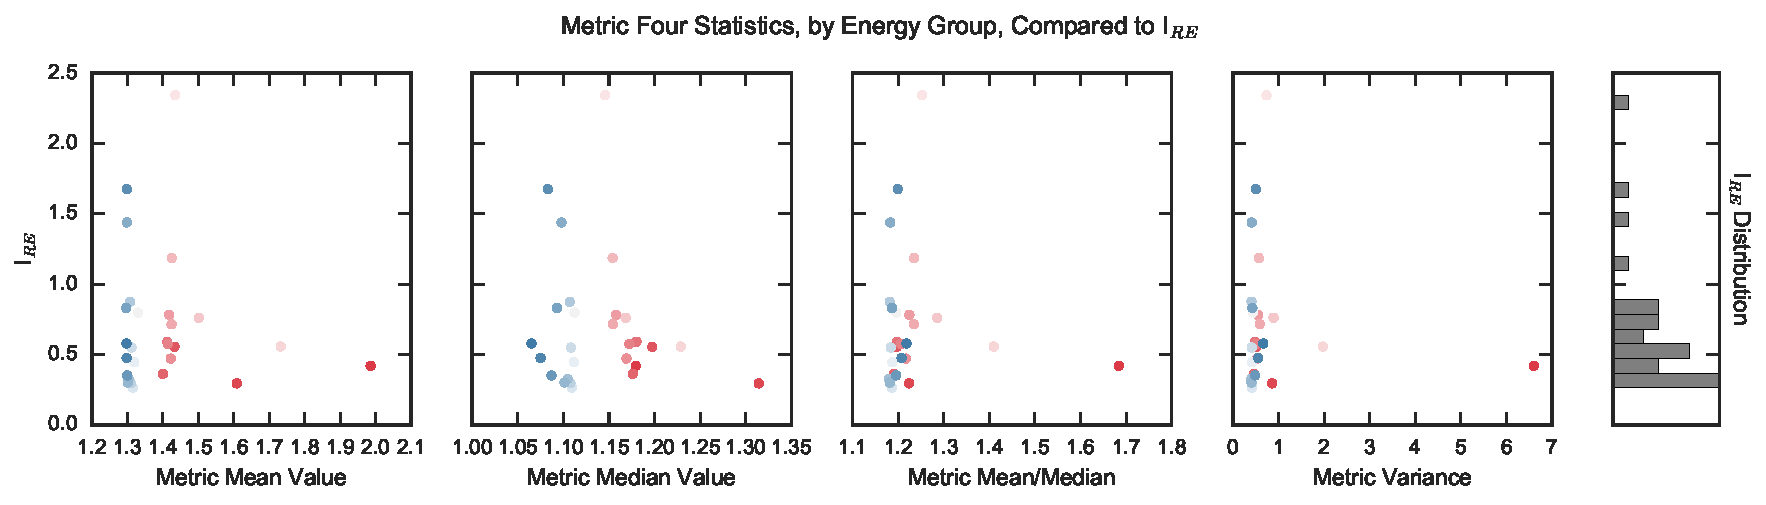
\includegraphics[width=\linewidth]{./chapters/characterization_probs/figures/char/prob1v1/metric_four_err_stats_mean.pdf}
    \caption{I$_{RE}$ for M$_4$ for air beam geometry}
    \label{fig:beamairIRE}
  \end{subfigure}
\end{figure}
\begin{figure}[htb!]\ContinuedFloat
  \centering
  \begin{subfigure}[t]{\textwidth}
    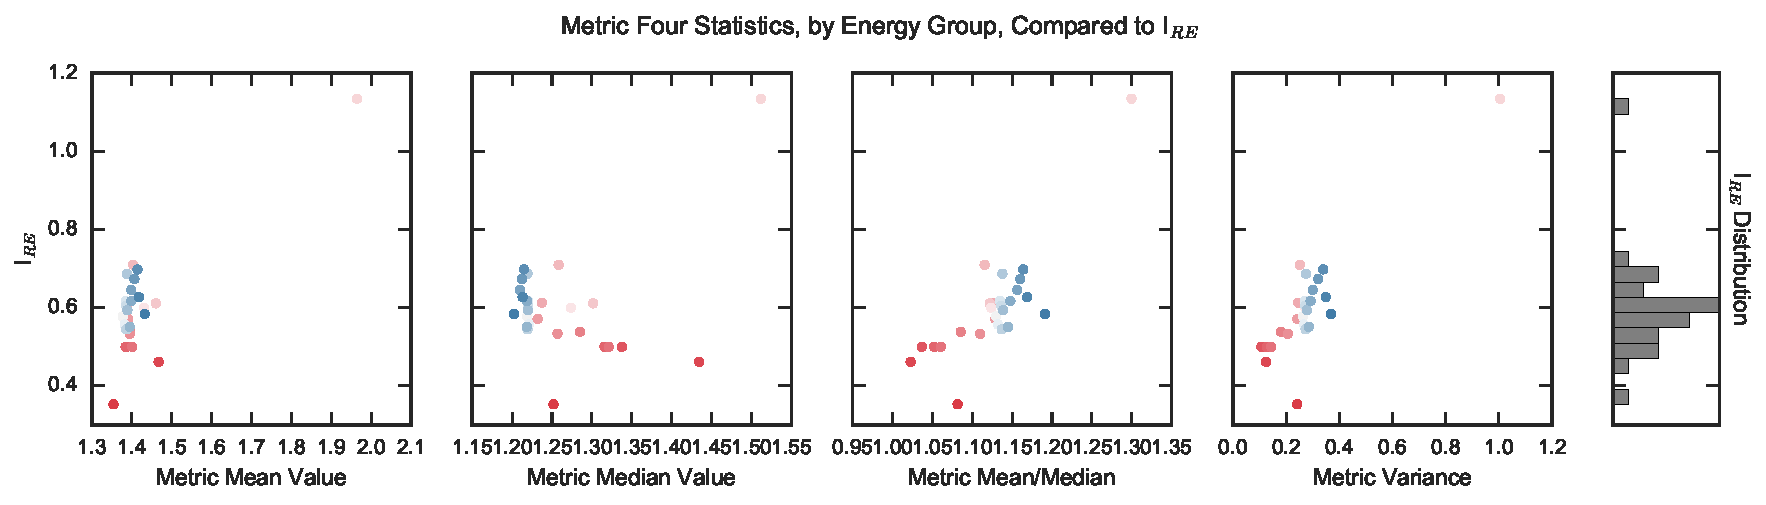
\includegraphics[width=\linewidth]{./chapters/characterization_probs/figures/char/prob1v2/metric_four_err_stats_mean.pdf}
    \caption{I$_{RE}$ for M$_4$ for concrete beam geometry}
    \label{fig:beamconcreteIRE}
  \end{subfigure}
  \caption[Scatterplots of values describing M$_4$ distribution against I$_{RE}$
  for steel beam problem geometry material variants.]{Scatterplots of values
    describing M$_4$ distribution against I$_{RE}$ for steel beam problem
    geometry material variants. As with the distributions in
    \ref{fig:beamviolins}, M$_4$ is based on values filtered out in cells
  located above the contributon flux average value. The values on the x-axes of
the figures are evaluated based on the subset of M$_4$ values. Coloring of
datapoints correspond to the energy groups.}
  \label{fig:beamIREs}
\end{figure}

Based on the violin plots in \ref{fig:beamviolins}, it was observed that
the M$_4$ distribution was far different in the air variant of this problem
geometry than the steel or concrete variants. This is also observable in Figure
\ref{fig:beamIREs}, which plots the relative error improvement metric, I$_{RE}$
with different metric distribution values. Recall that a low I$_{RE}$ means that
the $\Omega$ method achieved a superior relative error to standard CADIS.

Figures \ref{fig:beamsteelIRE} through \ref{fig:beamconcreteIRE} shows the
relative error improvement factors for each of the steel beam material variants
described in \ref{fig:beamviolins}. For both the steel and concrete problems,
CADIS-$\Omega$ has favorable values for I$_{RE}$ in most energy bins. In Figures
\ref{fig:beamsteelIRE} and \ref{fig:beamconcreteIRE} there appears to be a trend
in I$_{RE}$ with both the metric variance and the metric skew--the ratio of the
mean to the median values--which indicates that the metric distribution rather
than the metric average are more likely to be related to the improvement in the
relative error for these problems. This trend is not observable for the air
variant in Figure \ref{fig:beamairIRE}. In fact, the metric mean and median
values are better indicators for I$_{RE}$ than the distribution values.

Looking at the distributions of I$_{RE}$ it is clear that despite the similar
metric distribution values, the concrete and steel variants of this problem do
have different performances. Disregarding energy group 11, which is an outlier
in all three problem figures, the two problems have similar ranges of I$_{RE}$.
However, the highest energy groups have the lowest I$_{RE}$ for the concrete
problem, while the lowest values in the steel problem occur in in intermediate
energy groups.


\subsection{U-Shaped Corridor}
\label{subsec:resultsucorridor}

The U-shaped air corridor embedded in concrete
FOM and timing
results are summarized in Tables
\ref{tab:ucorridorfoms} and \ref{tab:ucorridortimes}. Figures
\ref{fig:ucorridorresult} and \ref{fig:ucorridorerror} show the results obtained
by the track length tally in CADIS, CADIS-$\Omega$ and the nonbiased analog
Monte Carlo.

\begin{table}[h!]
  \centering
  \begin{tabular}{lrrrrr}
\toprule
{} &  cadis &             & cadisangle &             & analog \\
{} &     MC & MC\_adjusted &         MC & MC\_adjusted &     MC \\
\midrule
tally avg   &   64.1 &        51.9 &       60.2 &        38.3 &  0.378 \\
max RE      & 0.0183 &      0.0148 &     0.0144 &     0.00913 & 0.0644 \\
min RE      &   14.9 &          12 &       13.4 &        8.54 &    -- \\
time (mins) &   54.6 &        67.5 &        188 &         296 &   15.5 \\
\bottomrule
\end{tabular}

  \caption[Figure of Merit comparison between methods for U-shaped air corridor in concrete.]
  {Figure of Merit comparison between methods for U-shaped air corridor in
  concrete.}
  \label{tab:ucorridorfoms}
\end{table}

\begin{table}[h!]
  \centering
  \begin{tabular}{llrrr}
\toprule
          &             &          CADIS & CADIS-$\Omega$ &         analog \\
        &              & \multicolumn{3}{c}{time (minutes)} \\
\midrule
MCNP time & total &          54.61 &         187.92 &          15.54 \\
deterministic time & advantg\_time &           0.19 &           0.21 &            -- \\
          & denovo\_time &          12.68 &         105.90 &            -- \\
          & dispose\_time &           0.01 &           0.35 &            -- \\
          & omega\_time &           0.00 &           1.49 &            -- \\
          & total &          12.87 &         107.60 &            -- \\
wall time &              &          67.48 &         295.52 &          15.54 \\
\bottomrule
\end{tabular}

  \caption[Detailed timing results for U-shaped air corridor in concrete.]
  {Detailed timing results for U-shaped air corridor in concrete.}
  \label{tab:ucorridortimes}
\end{table}

Much like the single- and multiple-turn labyrinths, the U-shaped air corridor
has a pathway of preferential movement for particles in a concrete shield. In
this problem, the particles travel down the legs of the u-bend to a detector on
the other side of the corridor. The particles should have preferential flowpaths
through the air ducts, but it is possible for low energy particles to traverse
the concrete barrier between the source and detector. The high energy particles
tallied in the detector are more likely to have traveled through the air ducts
and the low energy particles may be supplied from the shield or from scattering
down the air duct.

The FOM table for the u-shaped corridor shows that this is a fairly difficult
problem for CADIS, CADIS-$\Omega$, and the analog. For the tally average FOM,
CADIS and CADIS-$\Omega$ achieve a FOM two orders of magnitude higher than the
nonbiased analog. Both methods have comparable FOMs. In fact, CADIS and
CADIS-$\Omega$ are in relative agreement for all FOMs calculated with the Monte
Carlo runtime. Interestingly, the nonbiased analog Monte Carlo has a higher
maximum relative error FOM than either method. However, this analog tally for
this problem has many
nontallied bins (as can be gathered from the major discrepancy in results in
Figures \ref{fig:ucorridorresult} and \ref{fig:ucorridorerror}). For the
few bins that were tallied, the analog has a high FOM.

\begin{figure}[h!]
  \centering
  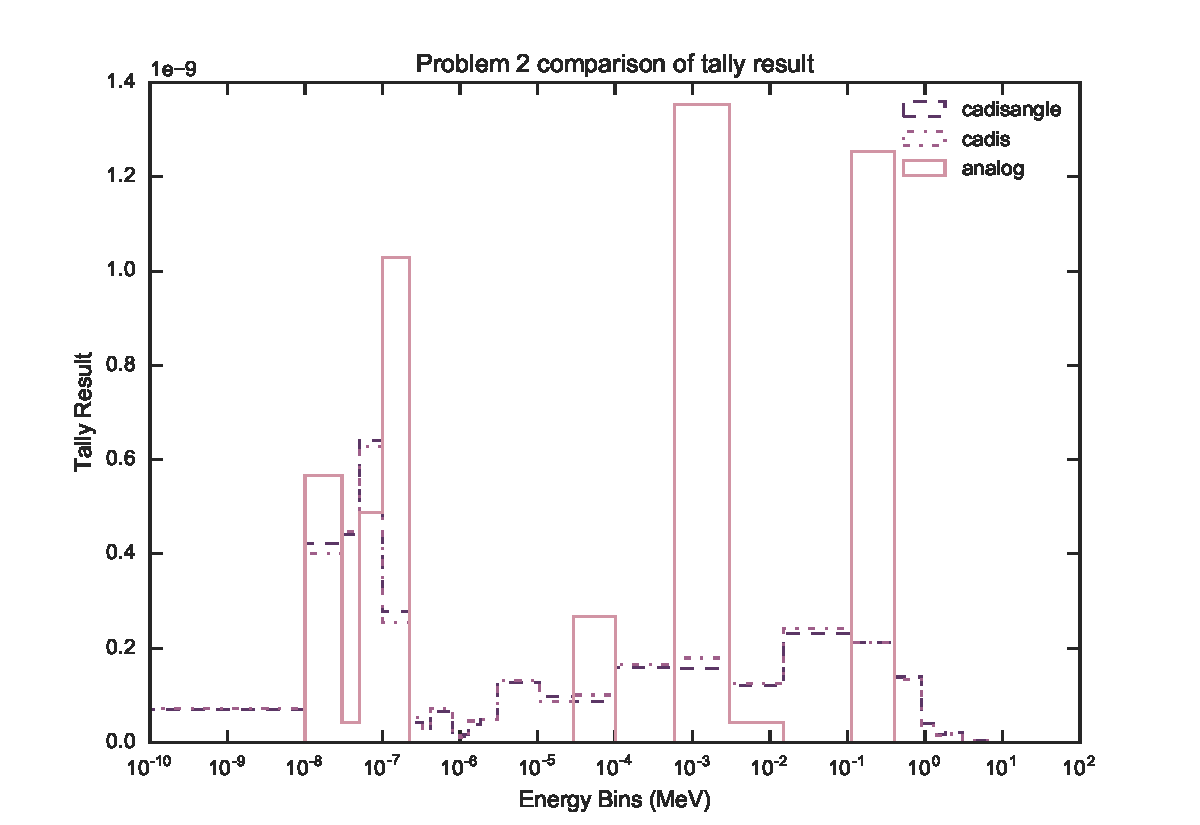
\includegraphics[height=10cm]{./chapters/characterization_probs/figures/char/prob_2/problem_2_tally_result_compare.pdf}
  \caption[Tally results comparison between methods for U-shaped air corridor in
  concrete.]
  {Tally results comparison between methods for U-shaped air corridor in
  concrete.}
  \label{fig:ucorridorresult}
\end{figure}

\begin{figure}[h!]
  \centering
  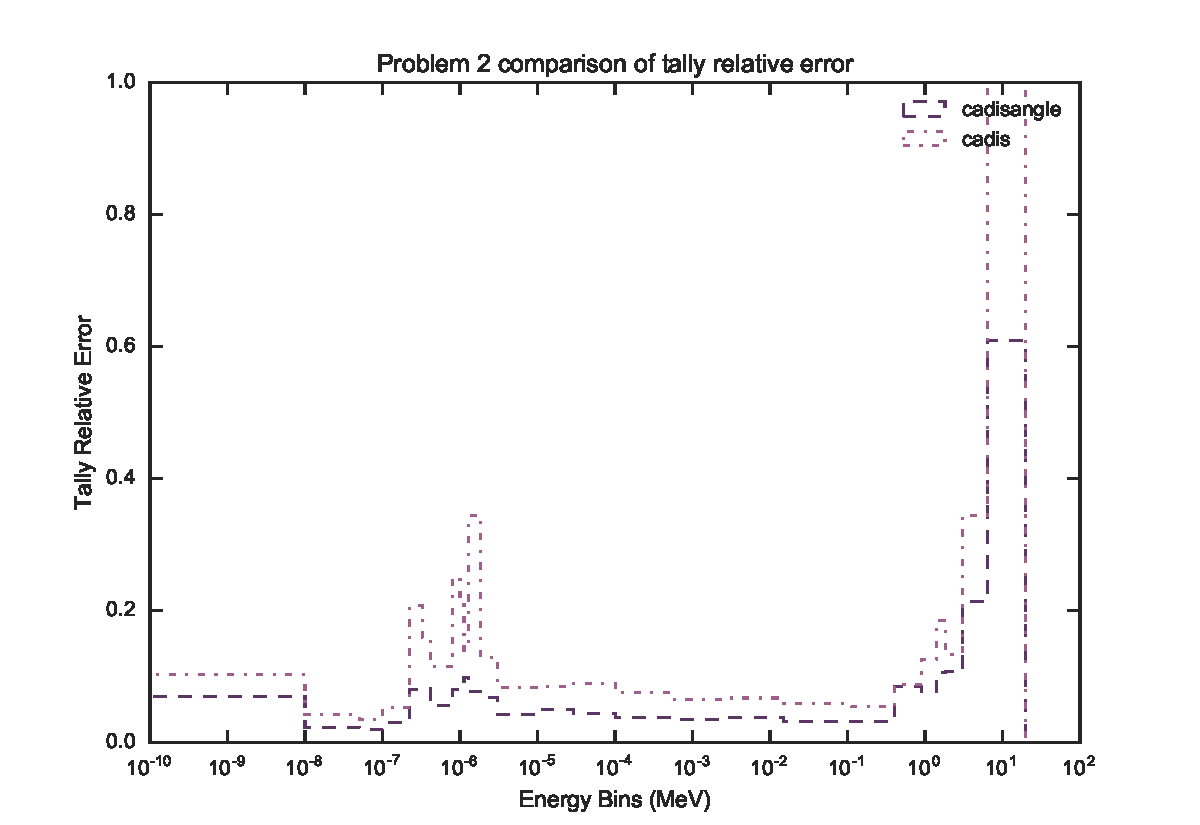
\includegraphics[height=10cm]{./chapters/characterization_probs/figures/char/prob_2/problem_2_tally_error_compare.pdf}
  \caption[Tally relative error comparison between methods for U-shaped air
  corridor in concrete.]
  {Tally relative error comparison between methods for U-shaped air corridor in
  concrete.}
  \label{fig:ucorridorerror}
\end{figure}

The tally results for the u-shaped corridor in Figure \ref{fig:ucorridorresult}
show general agreement between CADIS and CADIS-$\Omega$. The nonbiased analog
has no agreement with either method. Comparing their relative errors in Figure
\ref{fig:ucorridorerror}, we can gather that this is a difficult problem for
both methods. At high energies both CADIS and CADIS-$\Omega$ have very high
relative errors, indicating untrustworthy results. To get the relative error in
these regions for CADIS-$\Omega$ to below 0.10--a fairly standard threshold for
Monte Carlo--it would have to run nearly 40x longer, or ~900 hours. However,
CADIS-$\Omega$ achieves a uniformly lower relative error than CADIS for all
energy bins. Because the time to run CADIS-$\Omega$ is so much longer, the FOM
is impacted and appears worse than CADIS. Therefore, should CADIS-$\Omega$ use
the same runtime as CADIS, CADIS will achieve superior relative errors.
Conversely, if CADIS-$\Omega$ uses the same particle count as CADIS,
CADIS-$\Omega$ will achieve superior relative errors.

\begin{figure}[htb!]
  \centering
  \begin{subfigure}[t]{\textwidth}
    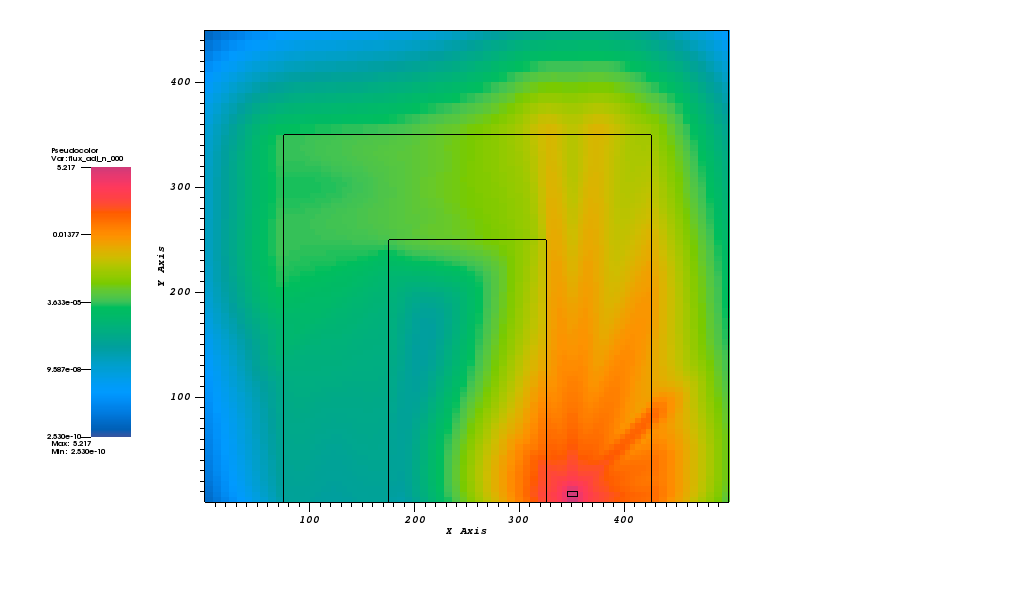
\includegraphics[width=0.9\linewidth]{./chapters/characterization_probs/figures/char/prob_2/prob2adjG00.png}
    \caption{Adjoint flux distribution, highest energy group}
    \label{fig:ubendadjflux}
  \end{subfigure}
\end{figure}
\begin{figure}[htb!]\ContinuedFloat
  \centering
  \begin{subfigure}[t]{\textwidth}
    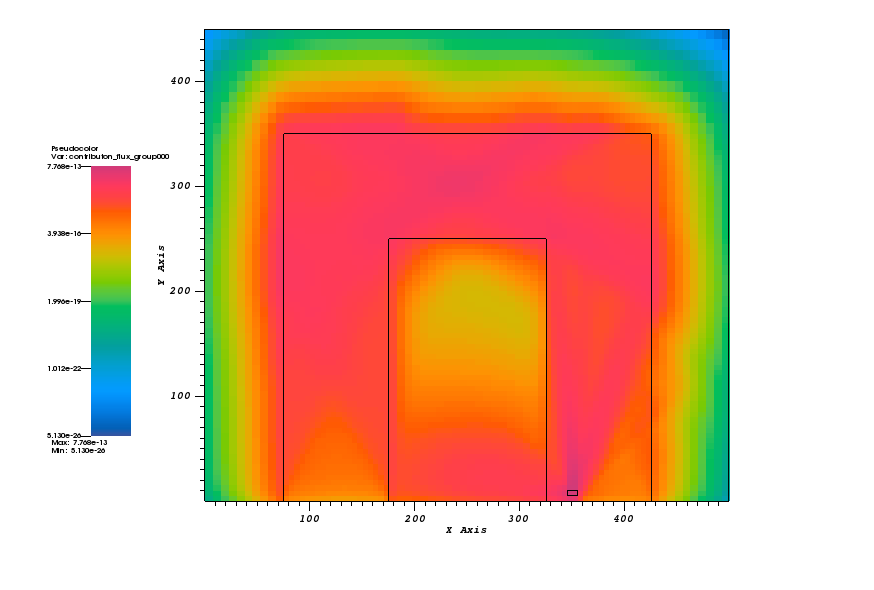
\includegraphics[width=0.9\linewidth]{./chapters/characterization_probs/figures/char/prob_2/prob2contribG00.png}
    \caption{Contributon flux distribution, highest energy group}
    \label{fig:ubendcontribflux}
  \end{subfigure}
\end{figure}
\begin{figure}[htb!]\ContinuedFloat
  \centering
  \begin{subfigure}[t]{\textwidth}
    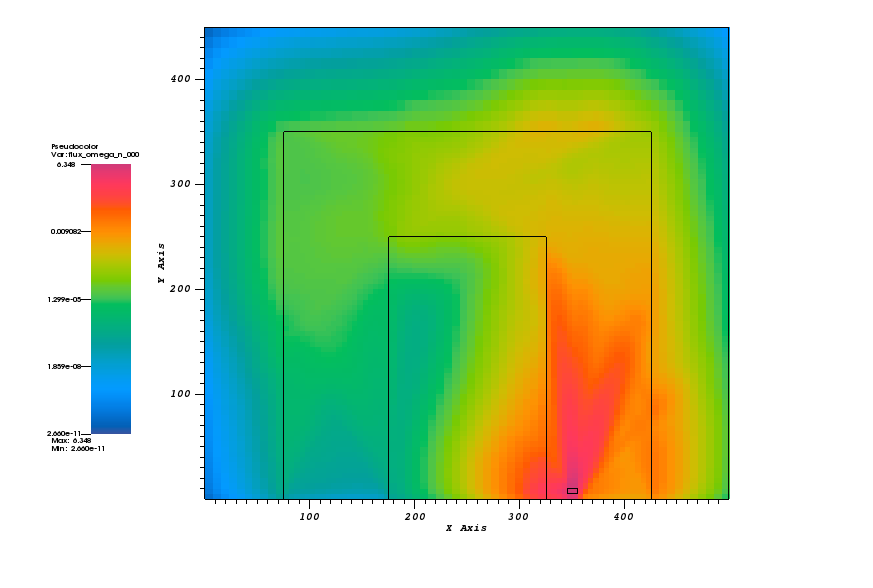
\includegraphics[width=0.9\linewidth]{./chapters/characterization_probs/figures/char/prob_2/prob2omegaG00.png}
    \caption{$\Omega$ flux distribution, highest energy group}
    \label{fig:ubendomegaflux}
  \end{subfigure}
  \caption[Flux distributions at problem midplane for U-shaped corridor.]{Flux
  distributions at problem midplane for U-shaped corridor. Distributions shown
are for the highest energy group. In this problem the forward source and
detector region are located in different z-plane locations.}
  \label{fig:ubendfluxes}
\end{figure}

While the u-shaped bend problem does not have FOMs for CADIS-$\Omega$ that
significantly improve upon CADIS', CADIS-$\Omega$ still achieved lower relative
errors than CADIS. Figure \ref{fig:ubendfluxes} shows the flux distributions in
the U-bend located at the midplane containing the NaI detector. Figure
\ref{fig:ubendadjflux} shows the adjoint scalar flux, Figure
\ref{fig:ubendcontribflux} shows the angle-integrated contributon scalar flux,
and Figure \ref{fig:ubendomegaflux} shows the $\Omega$-flux, all at the same
problem midplane.

As with the single-turn labyrinth, the adjoint scalar flux
in Figure \ref{fig:ubendadjflux} shows substantial ray effects
in the air regions near the adjoint source. As
expected, the ray effects are mitigated once the particles interact with
concrete. The difference in flux value between the orange region and the yellow
regions of the plot is on the order of two- to three- orders of magnitude. The
two ray effect fingers are separated by a distance of 10-20cm, meaning that a
particle traversing air in this region may experience fairly large differences
in importance between scattering events.

In this problem the forward source is offset in the z-plane from the detector by
100cm. The effects of this on the flux are visualized well by the contributon
flux in Figure \ref{fig:ubendcontribflux}. In the left-leg of the u-bend, the
contributon flux decreases near the bottom. This is because particles are more
biased in a deeper z-plane, towards the forward source. It is also clear from
this figure that in the high energy region, the contributon flux streams
particles through the concrete shield.

The $\Omega$-flux shown in Figure \ref{fig:ubendomegaflux} does not attempt to
force particles through the shield like the contributon flux, nor does it have
as substantial of ray effects as the adjoint scalar flux distribution. However,
the ray effects in this variant are not completely mitigated. There appears to
be a cone of particles extending into the u-bend that are of greater importance
than the other regions near the detector. This is a clear effect of the forward
flux distribution. However, the region just to the right of the detector
location is of possible consequence. Between the detector and directly to the
right, the flux decreases in magnitude more than two orders of magnitude. It is
possible that the large gradient in importnace could be adversely affecting the
time achieved by the $\Omega$ methods for this problem.

\begin{figure}[htb!]
  \centering
  \begin{subfigure}[t]{\textwidth}
    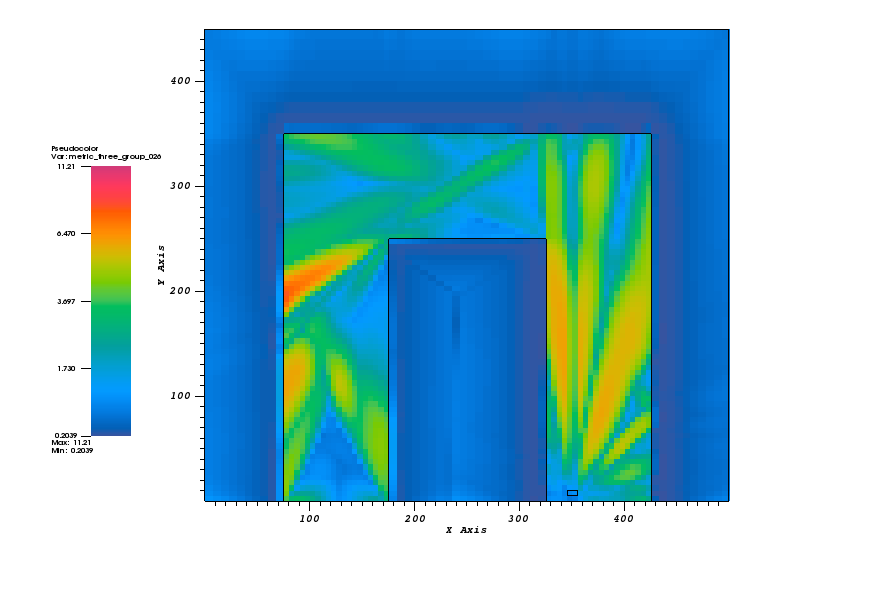
\includegraphics[width=0.9\linewidth]{./chapters/characterization_probs/figures/char/prob_2/prob2M3G26.png}
    \caption{M$_3$ distribution, visualized in plane containing detector}
    \label{fig:ubendM3}
  \end{subfigure}
\end{figure}
\begin{figure}[htb!]\ContinuedFloat
  \centering
  \begin{subfigure}[t]{\textwidth}
    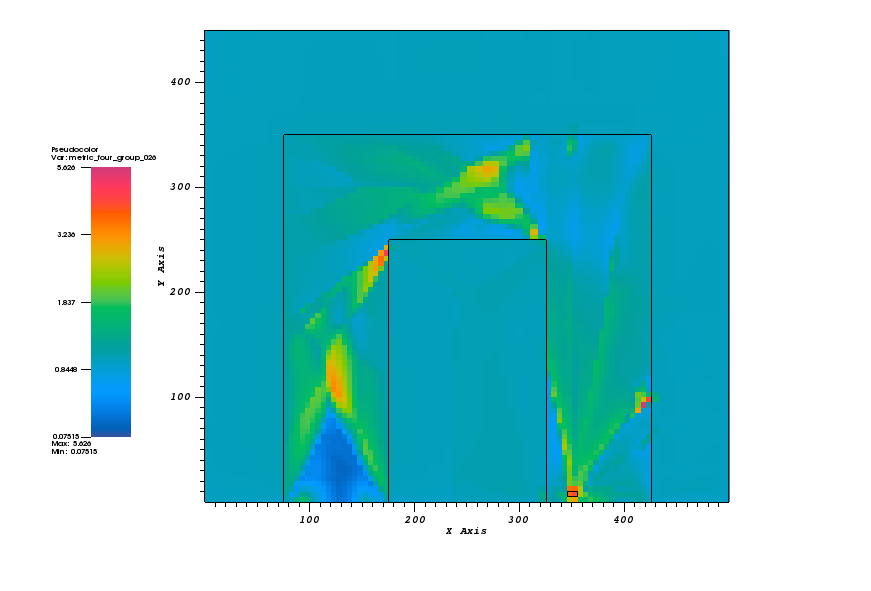
\includegraphics[width=0.9\linewidth]{./chapters/characterization_probs/figures/char/prob_2/prob2M4G26.png}
    \caption{M$_4$ distribution, visualized in plane containing detector}
    \label{fig:ubendM4}
  \end{subfigure}
  \caption[Anisotropy metrics plotted at problem midplane for U-shaped
  corridor.]{Anisotropy metrics plotted at problem midplane for U-shaped
    corridor. Energy group shown is for lowest energy}
  \label{fig:ubendmetrics}
\end{figure}

Figures \ref{fig:ubendM3} and \ref{fig:ubendM4} show the anisotropy metrics for
the u-shaped bend. Figure \ref{fig:ubendM3} shows the M$_3$ distribution, which
as one may recall is the ratio of the contributon maximum angular flux to the
contributon average angular flux in the cell. M$_4$, which is visualized in
Figure \ref{fig:ubendM4}, divides M$_3$ by the ratio of the maximum to average
adjoint angular fluxes.

Comparing these two figures we can identify the effect
of this normalization on the anisotropy metrics. Beginning with the M$_3$
distribution plot in Figure \ref{fig:ubendM3}, it is clear that we still observe
the secondary ray effects in the flux anisotropies that were observed in the
labyrinth problems. On the right side of the u-bend, we observe ray effects in
the aniostropy that are likely from the adjoint flux distribution. On the left
side of the bend we observe oblong circular distributions of anisotropy. These
are more likely to be from particles emanating forward source distribution. The
contributon flux anisotropies are much stronger in the air channels than in the
concrete shield, as we would expect. In the shield immediately bounding the air,
we observe a fairly isotropic flux distribution, but as particles reach closer
to the edges the anisotropy increases slightly.

The M$_4$ distributions shown in \ref{fig:ubendM4} show how certain features of
the anisotropy are removed when using the control adjoint angular flux. In
particular, the shield region becomes completely normalized, meaning that the
isotropy in the contributon flux matches that of the adjoint flux. The air
regions are where real and substantial differences occur. In particular, we see
peaks in the anisotropy where the forward and adjoint fluxes meet. At the top of
the bend, the adjoint and forward fluxes have scattered relatively few times and
thus generate a high aniosotropy in the contributon flux.

These anisotropy plots illustrate how in certain regions the flux anisotropy may
be very high. Further, they show regions where the fluxes strongly interact with
one another. In addition to helping to quantify the effectiveness of the method,
they reveal interesting features of the solution that may not be obvious using
standard flux figures.

\subsection{Shielding with Rebar}
\label{subsec:resultrebar}

The problem with rebar embedded both in the x- and y- directions
in concrete has
results summarized in Tables
\ref{tab:rebarfoms} and \ref{tab:rebartimes}. Figures
\ref{fig:rebarresult} and \ref{fig:rebarerror} show the results obtained
by the track length tally in CADIS, CADIS-$\Omega$ and the nonbiased analog
Monte Carlo.

\begin{table}[h!]
  \centering
  \begin{tabular}{lrrrrr}
\toprule
{} & \multicolumn{2}{c}{CADIS}   & \multicolumn{2}{c}{CADIS-$\Omega$}  & analog \\
{} &    MC & MC$_{hybrid}$ &         MC & MC$_{hybrid}$ &     MC \\
\midrule
tally avg   &   1.15 &        1.09 &     0.0136 &      0.0127 &  0.948 \\
max RE      & 0.0345 &      0.0327 &    0.00117 &     0.00109 & 0.0186 \\
min RE      &    235 &         223 &        199 &         186 &    -- \\
time (mins) &    328 &         346 &   1.55e+03 &    1.66e+03 &   53.8 \\
\bottomrule
\end{tabular}

  \caption[Figure of Merit comparison between methods for rebar-embedded
  concrete.]{Figure of Merit comparison between methods for rebar-embedded
  concrete.}
  \label{tab:rebarfoms}
\end{table}

\begin{table}[h!]
  \centering
  \begin{tabular}{llrrr}
\toprule
          &              &          cadis &     cadisangle &         analog \\
          &              & time (minutes) & time (minutes) & time (minutes) \\
\midrule
MCNP time & total &         327.81 &        1550.54 &          53.82 \\
deterministic time & advantg\_time &           0.28 &           0.29 &            -- \\
          & denovo\_time &          17.70 &         105.09 &            -- \\
          & dispose\_time &           0.03 &           0.41 &            -- \\
          & omega\_time &           0.00 &           2.05 &            -- \\
          & total &          17.98 &         107.43 &            -- \\
wall time &              &         345.79 &        1657.97 &          53.82 \\
\bottomrule
\end{tabular}

  \caption[Detailed timing results for rebar-embedded concrete]
  {Detailed timing results for rebar-embedded concrete.}
  \label{tab:rebartimes}
\end{table}

The FOM results for the rebar-embedded concrete show that this is a very poor
problem for CADIS-$\Omega$, in general. CADIS-$\Omega$ has lower FOMs than CADIS
in all measures. CADIS-$\Omega$ spends fractionally over five--both
deterministically and in Monte Carlo--the
transport time that CADIS does. Further, CADIS-$\Omega$ has poorer FOMs in both
the tally average and maximum relative error than the nonbiased analog. This is
due to CADIS-$\Omega$ requiring nearly 30x longer to run Monte Carlo than the
nonbiased analog.

\begin{figure}[h!]
  \centering
  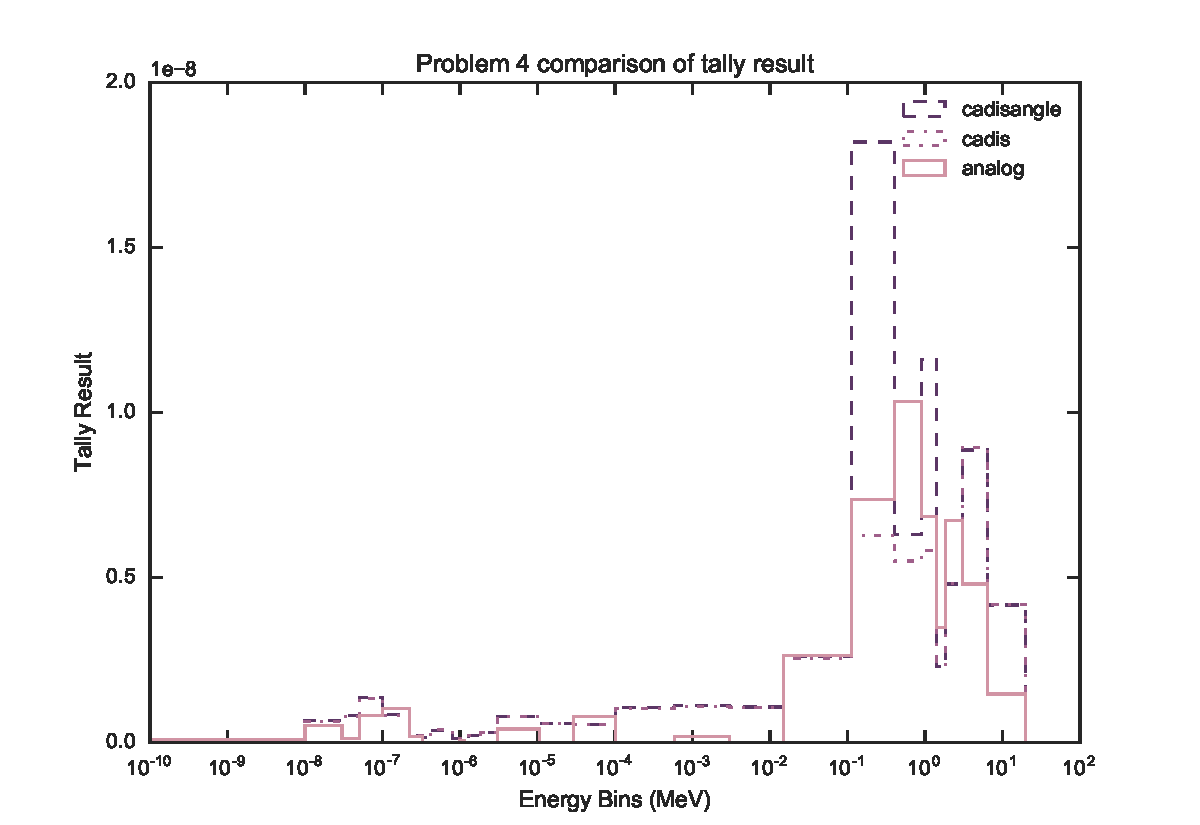
\includegraphics[height=10cm]{./chapters/characterization_probs/figures/char/prob_4/problem_4_tally_result_compare.pdf}
  \caption[Tally results comparison between methods for rebar-embedded concrete.]
  {Tally results comparison between methods for rebar-embedded concrete.}
  \label{fig:rebarresult}
\end{figure}

\begin{figure}[h!]
  \centering
  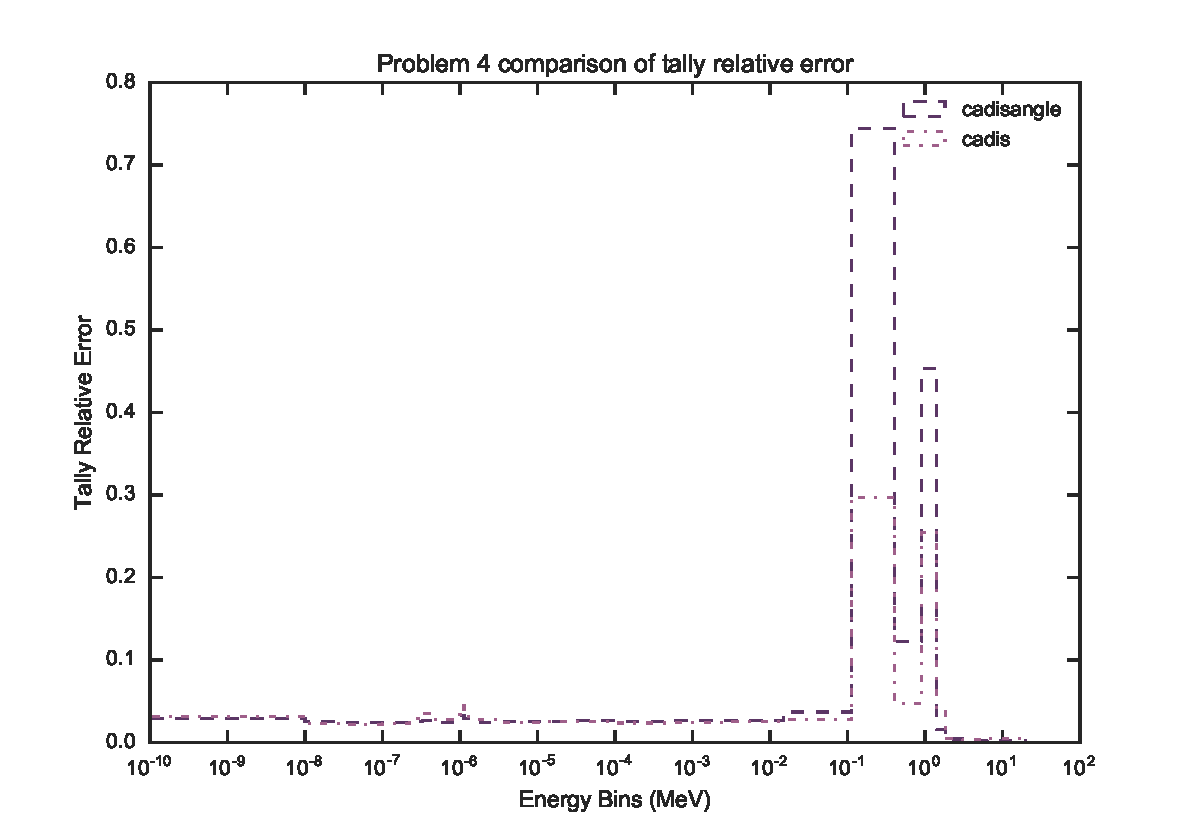
\includegraphics[height=10cm]{./chapters/characterization_probs/figures/char/prob_4/problem_4_tally_error_compare.pdf}
  \caption[Tally relative error comparison between methods for rebar-embedded concrete.]
  {Tally relative error comparison between methods for rebar-embedded concrete.}
  \label{fig:rebarerror}
\end{figure}

Figure \ref{fig:rebarresult} shows that the tally results for the rebar-embedded
concrete do not generally agree between any method. CADIS and CADIS-$\Omega$
have better agreement with each other than with the nonbiased analog, but at
high energies their results differ significantly. However, in comparing their
relative errors in Figure \ref{fig:rebarerror}, the large discrepancy in their
results is explained by the very high relative errors in this region. As with
the u-shaped air corridor, neither method achieves satisfactory relative errors
below 0.10 in high energy bins. However, both methods achieve comparitavely good
relative error results in energy bins below $10^{-1}$ MeV.

Unlike previous problems that had
significant problem volumes filled with air, this particular problem has a thick
shield with which incident particles must interact. While this problem may
appear similar geometrically to the beam embedded in
concrete, this problem has far more preferential flowpaths by which particles
might flow. Some of these flowpaths are directed perpindicularly to a path
towards the detector. It is possible that CADIS-$\Omega$ is capturing these
flowpaths, but because they are not towards the detector CADIS-$\Omega$ spends a
significant portion of its time sampling less useful regions.

\begin{figure}[htb!]
  \centering
  \begin{subfigure}[t]{\textwidth}
    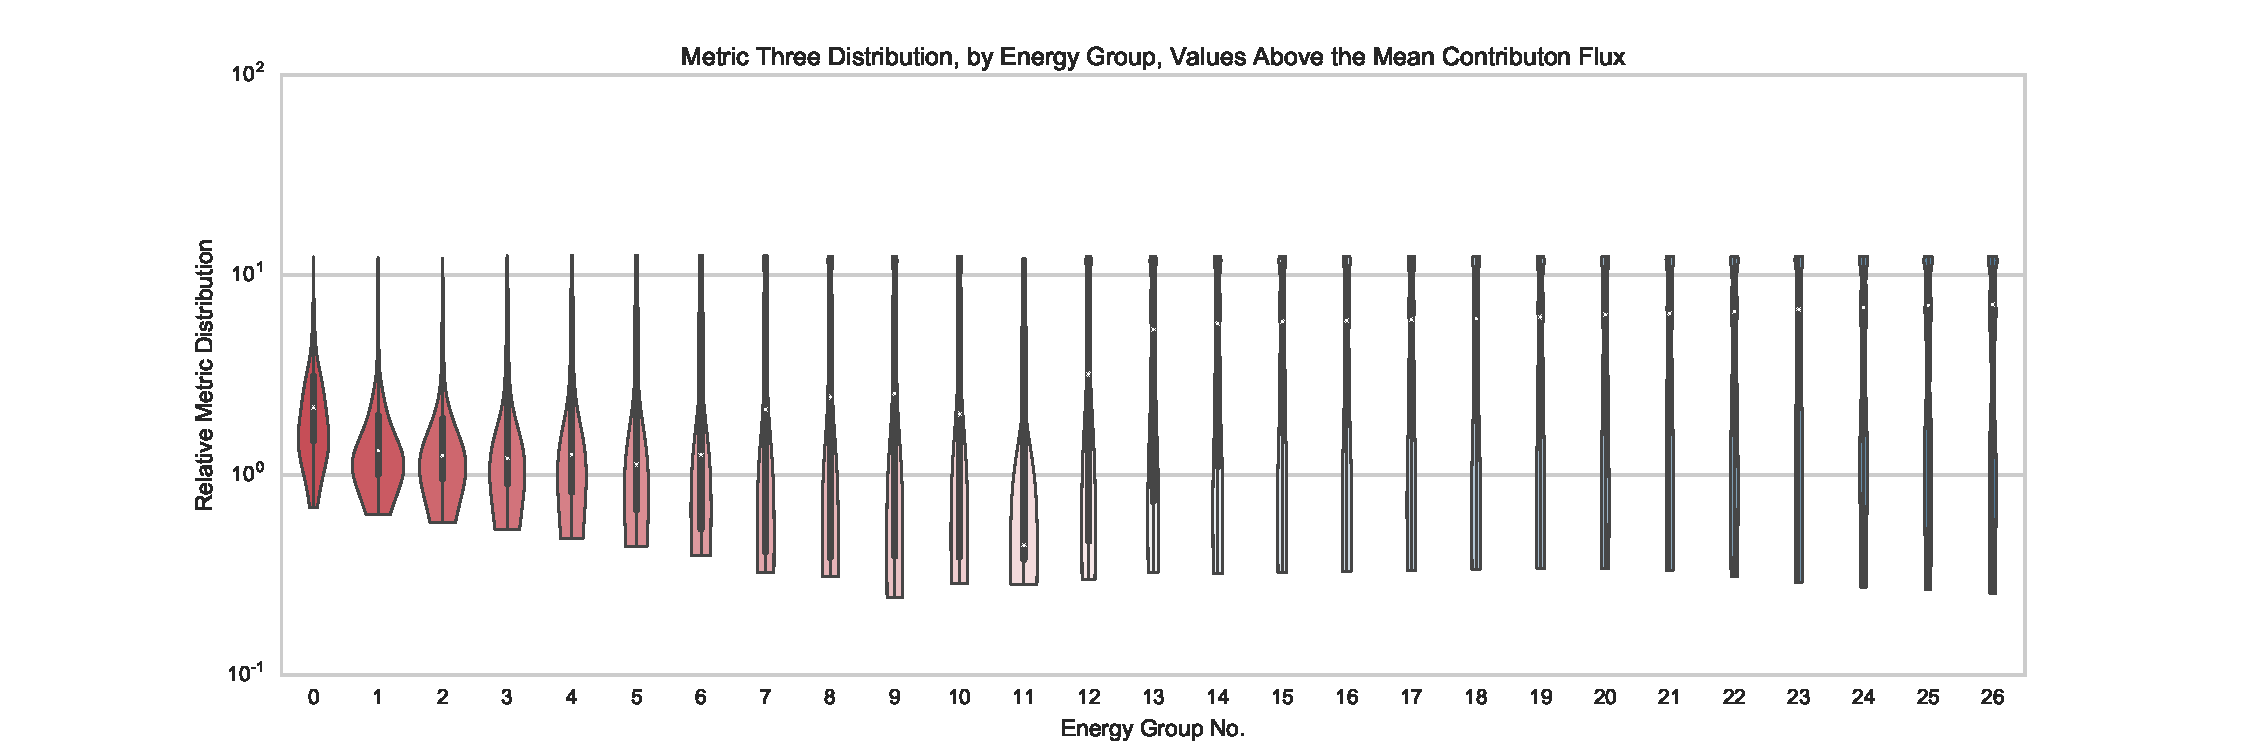
\includegraphics[width=\linewidth]{./chapters/characterization_probs/figures/char/prob_4/metric_three_violin_mean.pdf}
    \caption{M$_3$ distributions rebar embedded in concrete}
    \label{fig:M3violinrebar}
  \end{subfigure}
\end{figure}
\begin{figure}[htb!]\ContinuedFloat
  \centering
  \begin{subfigure}[t]{\textwidth}
    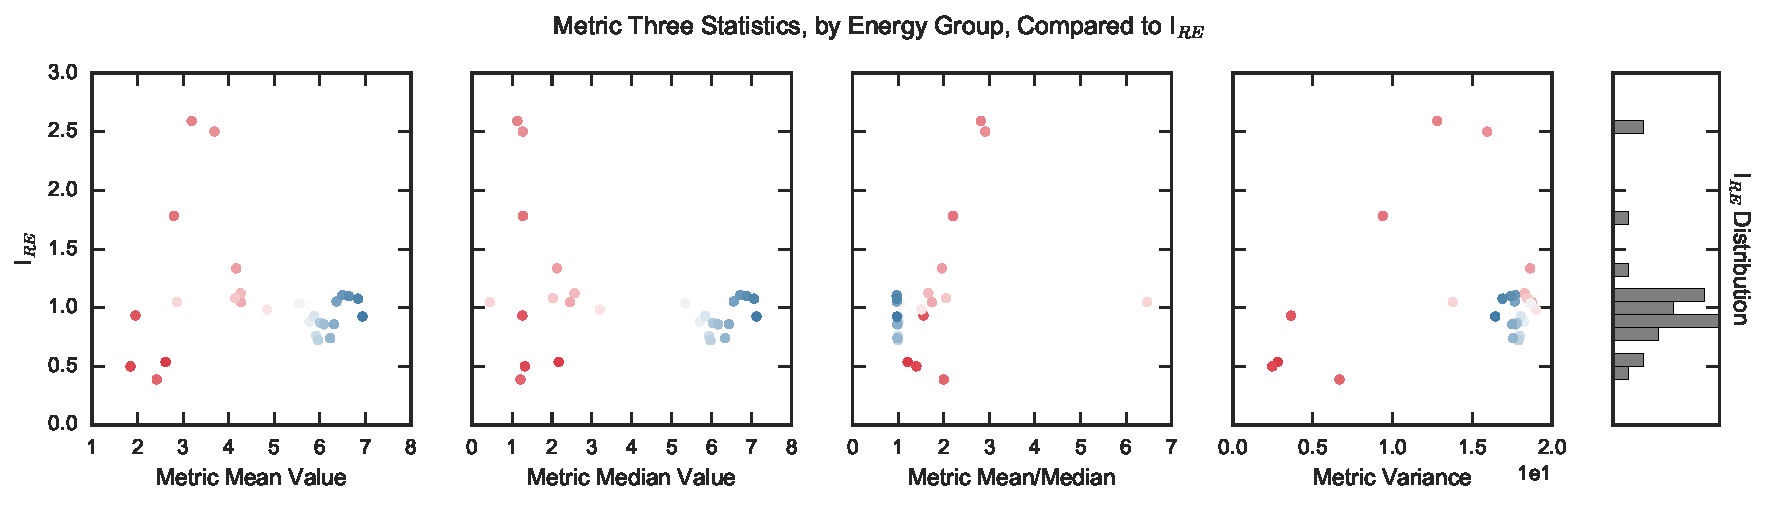
\includegraphics[width=\linewidth]{./chapters/characterization_probs/figures/char/prob_4/metric_three_err_stats_mean.pdf}
    \caption{I$_{RE}$ for M$_3$ for rebar embedded in concrete.}
    \label{fig:M3statsrebar}
  \end{subfigure}
  \caption[M$_3$ distribution and trends for rebar-embedded concrete
  problem.]{M$_3$ distribution and I$_{RE}$ scatterplot for rebar-embedded in
concrete. Values of M$_3$ have been filtered to be from cells that are above the
contributon mean value.}
  \label{fig:rebarplots}
\end{figure}

After inspecting the metric distributions against I$_{RE}$ and I$_{FOM}$, no
distinct trends were observable with any metric and either improvement factor.
The distribution with the best trends are included in Figure
\ref{fig:rebarplots}. Figure \ref{fig:M3violinrebar} illustrates the
metric distribution and Figure \ref{fig:M3statsrebar} shows the relative error
improvement metric as a function of different metric distribution values.

Figure \ref{fig:M3violinrebar} shows the metric
distribution for this problem using metric values from cells above the
contributon mean. It is clear from this distribution that low energy cells have
a large spread but no centering value. There exist some very anisotropic cells
at low energy groups, but there exist also exist some very isotropic cells.
Conversely, in high energy groups the metric distribution has a very clumped
distribution of values where the contributon max angular flux is higher than the
average contributon angular flux in the cell.

Using values that can be computed from the distributions shown in Figure
\ref{fig:M3violinrebar}, the relative error improvement between CADIS-$\Omega$
and CADIS can be plotted as shown in \ref{fig:M3statsrebar}. In general there
exist many energy bins where CADIS-$\Omega$ achieves a poorer relative error
than CADIS. The bins where the comparative error is the worst is in intermediate
energy regions. At low energy regions the relative errors are comparable, but as
shown in the timing table, the FOM will be much lower for CADIS-$\Omega$. There
does appear to be a slight trend in I$_{RE}$ with the ratio of the metric mean
to the metric median and with the metric variance. As with the steel beam
problem, this shows that the metric distribution is a better predictor of the
improvement in the relative error than the metric average or median value.
However, these trends are not strong, and it would be difficult to predict the
performance of a similar problem based on metric distributions.

It is possible that the filter matrix is not fine enough for this particular
problem to pull out metric
values of high importance, but even values filtered out above the mean
contributon flux did not have strong correlations. However, with the cutoffs
appearing in the distributions of \ref{fig:M3violinrebar}, choosing too high of
a filter value may also remove much of the metric distribution.

\subsection{Beam Problem}
\label{subsec:resultsbeam}

The nuclear physics beamline toy problem has FOM and timing
results summarized in Tables
\ref{tab:beamfoms} and \ref{tab:beamtimes}. Figures
\ref{fig:beamresult} and \ref{fig:beamerror} show the results obtained
by the track length tally in CADIS, CADIS-$\Omega$ and the nonbiased analog
Monte Carlo.

\begin{table}[h!]
  \centering
  \begin{tabular}{lrrrrr}
\toprule
{} & cadis &             & cadisangle &             & analog \\
{} &    MC & MC\_adjusted &         MC & MC\_adjusted &     MC \\
\midrule
tally avg   &   368 &         138 &       94.8 &        7.91 &    317 \\
max RE      & 0.542 &       0.202 &       1.18 &      0.0984 &    1.6 \\
min RE      &   -- &         -- &        -- &         -- &    -- \\
time (mins) &  2.23 &        5.97 &       1.69 &        20.3 &   1.69 \\
\bottomrule
\end{tabular}

  \caption[Figure of Merit comparison between methods for simplified
    experimental nuclear physics beamline.]
    {Figure of Merit comparison between methods for simplified experimental
    nuclear physics beamline.}
  \label{tab:beamfoms}
\end{table}

\begin{table}[h!]
  \centering
  \begin{tabular}{llrrr}
\toprule
          &             &          CADIS & CADIS-$\Omega$ &         analog \\
        &              & \multicolumn{3}{c}{time (minutes)} \\
\midrule
MCNP time & total &           2.23 &           1.69 &           1.69 \\
deterministic time & advantg\_time &           0.17 &           0.15 &            -- \\
          & denovo\_time &           3.57 &          17.88 &            -- \\
          & dispose\_time &           0.00 &           0.12 &            -- \\
          & omega\_time &           0.00 &           0.53 &            -- \\
          & total &           3.74 &          18.56 &            -- \\
wall time &              &           5.97 &          20.25 &           1.69 \\
\bottomrule
\end{tabular}

  \caption[Detailed timing results for simplified experimental nuclear physics
  beamline.]
  {Detailed timing results for simplified experimental nuclear physics beamline.}
  \label{tab:beamtimes}
\end{table}

The experimental nuclear physics beamline problem is the most
difficult of the characterization problems for both CADIS and CADIS-$\Omega$.
There are no walls off which
particles may scatter; the only places most particles will scatter is in the
detector regions and potentially off of air. These particular problems were run
with $1e9$ particles rather than $1e7$. Because there are so few interaction
points, the majority of particles leak out of the problem boundary so
more source particles are required to obtain results.

Table \ref{tab:beamfoms} shows that nuclear physics experimental beamline
problem has very slow convergence for
CADIS and CADIS-$\Omega$. CADIS, CADIS-$\Omega$ and the nonbiased analog all have
zero-scoring tally bins. These are in low energy regions, energy regions in
which particles in the problem never reach.
The maximum relative error FOM for CADIS, CADIS-$\Omega$,
and the nonbiased analog are all very low, indicating that the threshold for
convergence of the highest energy bin will take a long time for all three
methods. Interestingly, CADIS performs worse than CADIS-$\Omega$ and the
nonbiased analog with this metric. The nonbiased analog achieves the highest
maximum relative error FOM and the highest tally average relative error FOM for all
three methods.

A notable feature of Table \ref{tab:beamtimes} is the Monte Carlo runtime of
CADIS, CADIS-$\Omega$, and the nobiased analog. In previous characterization
problems, CADIS-$\Omega$ and CADIS had much longer runtimes than the nonbiased
analog. In all of the previous characterization problems, CADIS-$\Omega$ had a
longer runtime than CADIS. In this problem, CADIS-$\Omega$ has a shorter runtime
than CADIS. The deterministic runtime of CADIS-$\Omega$ relative to CADIS
is comparable to previous problems. A potential reason that the runtimes of
CADIS and CADIS-$\Omega$ is so close to the nonbiased analog is because so many
particles leak out of the problem space.
% Further, the reason that CADIS-$\Omega$
% may have a shorter runtime than CADIS is because ray effects are dampened in the
% problem. As a result, unphysical fluctuations in the flux that may generate
% additional sampling issues are eliminated with CADIS-$\Omega$.

\begin{figure}[h!]
  \centering
  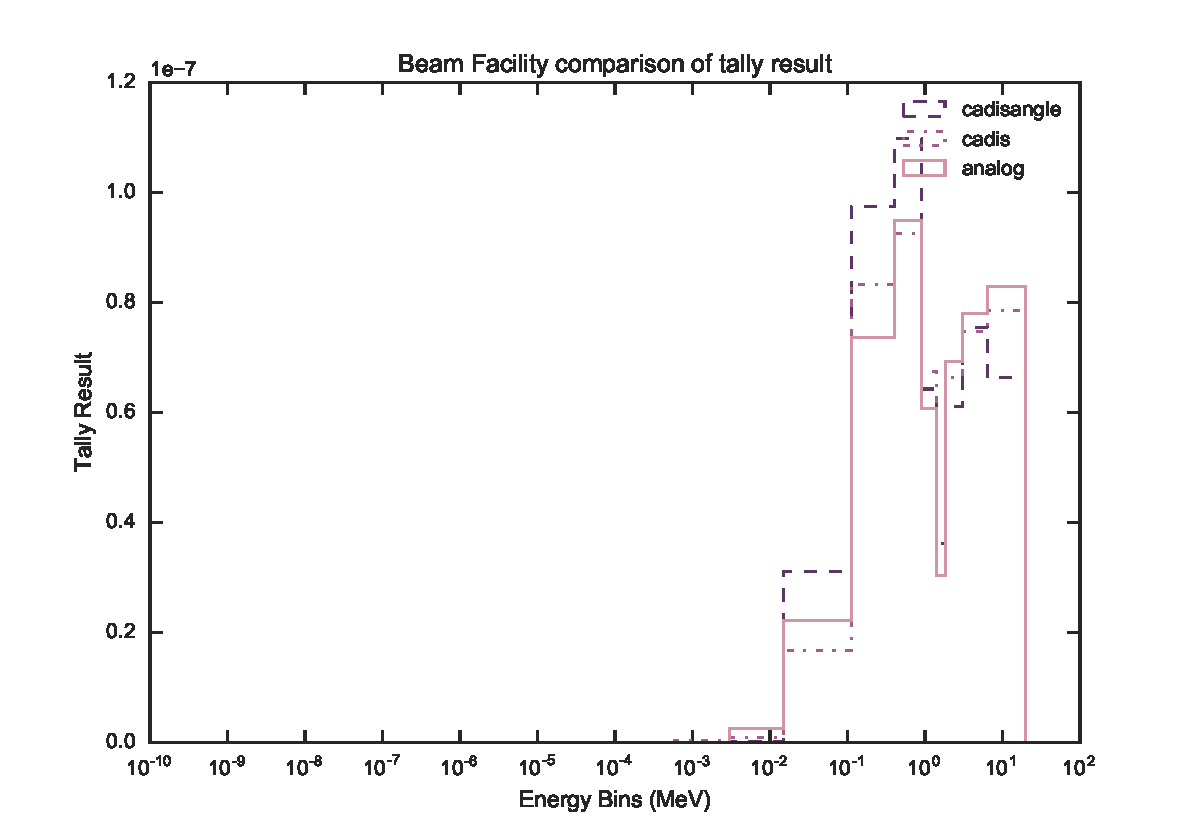
\includegraphics[height=10cm]{./chapters/characterization_probs/figures/char/beam/beam_facility_tally_result_compare.pdf}
  \caption[Tally results comparison between methods for simplified experimental
    nuclear physics beamline.]
  {Tally results comparison between methods for simplified experimental
    nuclear physics beamline.}
  \label{fig:beamresult}
\end{figure}

\begin{figure}[h!]
  \centering
  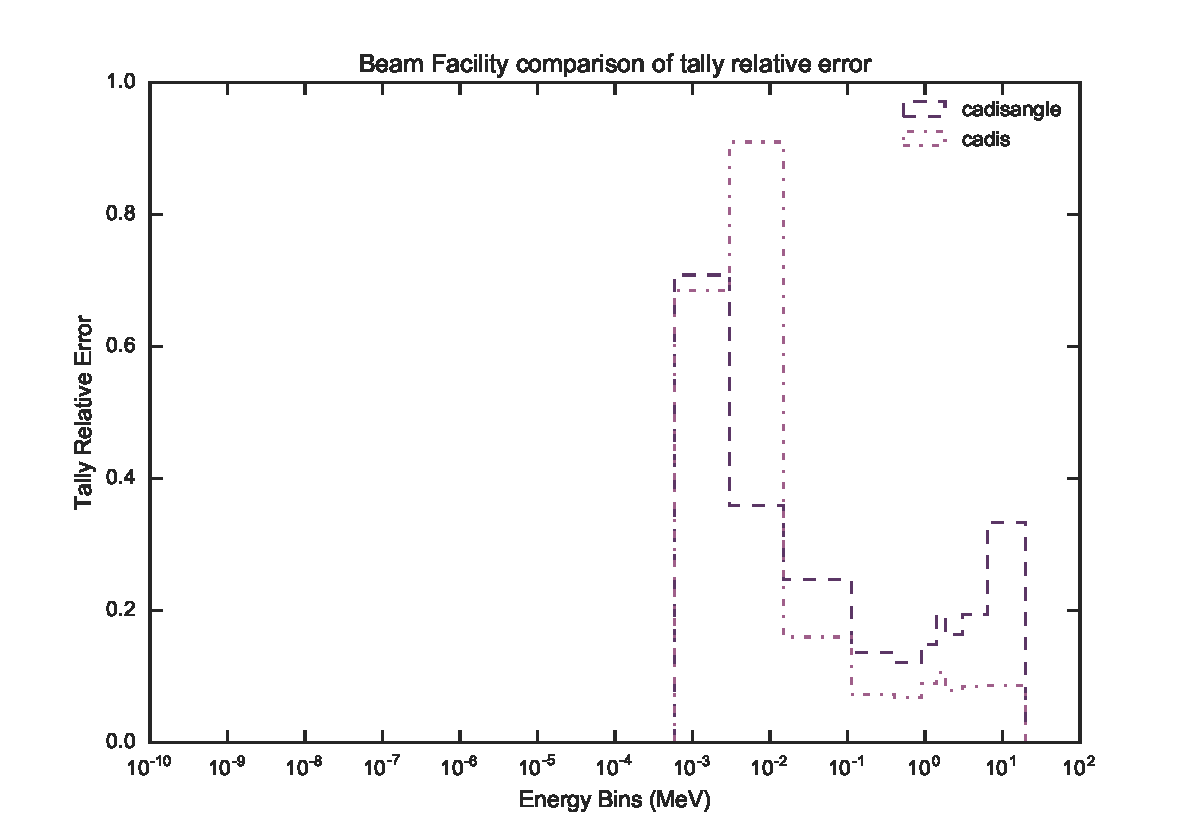
\includegraphics[height=10cm]{./chapters/characterization_probs/figures/char/beam/beam_facility_tally_error_compare.pdf}
  \caption[Tally relative error comparison between methods
    for simplified experimental nuclear physics beamline.]
  {Tally relative error comparison between methods for simplified experimental
    nuclear physics beamline.}
  \label{fig:beamerror}
\end{figure}

Comparing the full tally results presented in Figures \ref{fig:beamresult} and
\ref{fig:beamerror}, the FOM results from Table \ref{tab:beamfoms} have more
context. Figure \ref{fig:beamresult} shows that all three methods have similar
results in the track length tally. In a few of the bins CADIS and the nonbiased
analog appear to have closer results than CADIS and CADIS-$\Omega$.

\begin{figure}[htb!]
  \centering
  \begin{subfigure}[t]{\textwidth}
    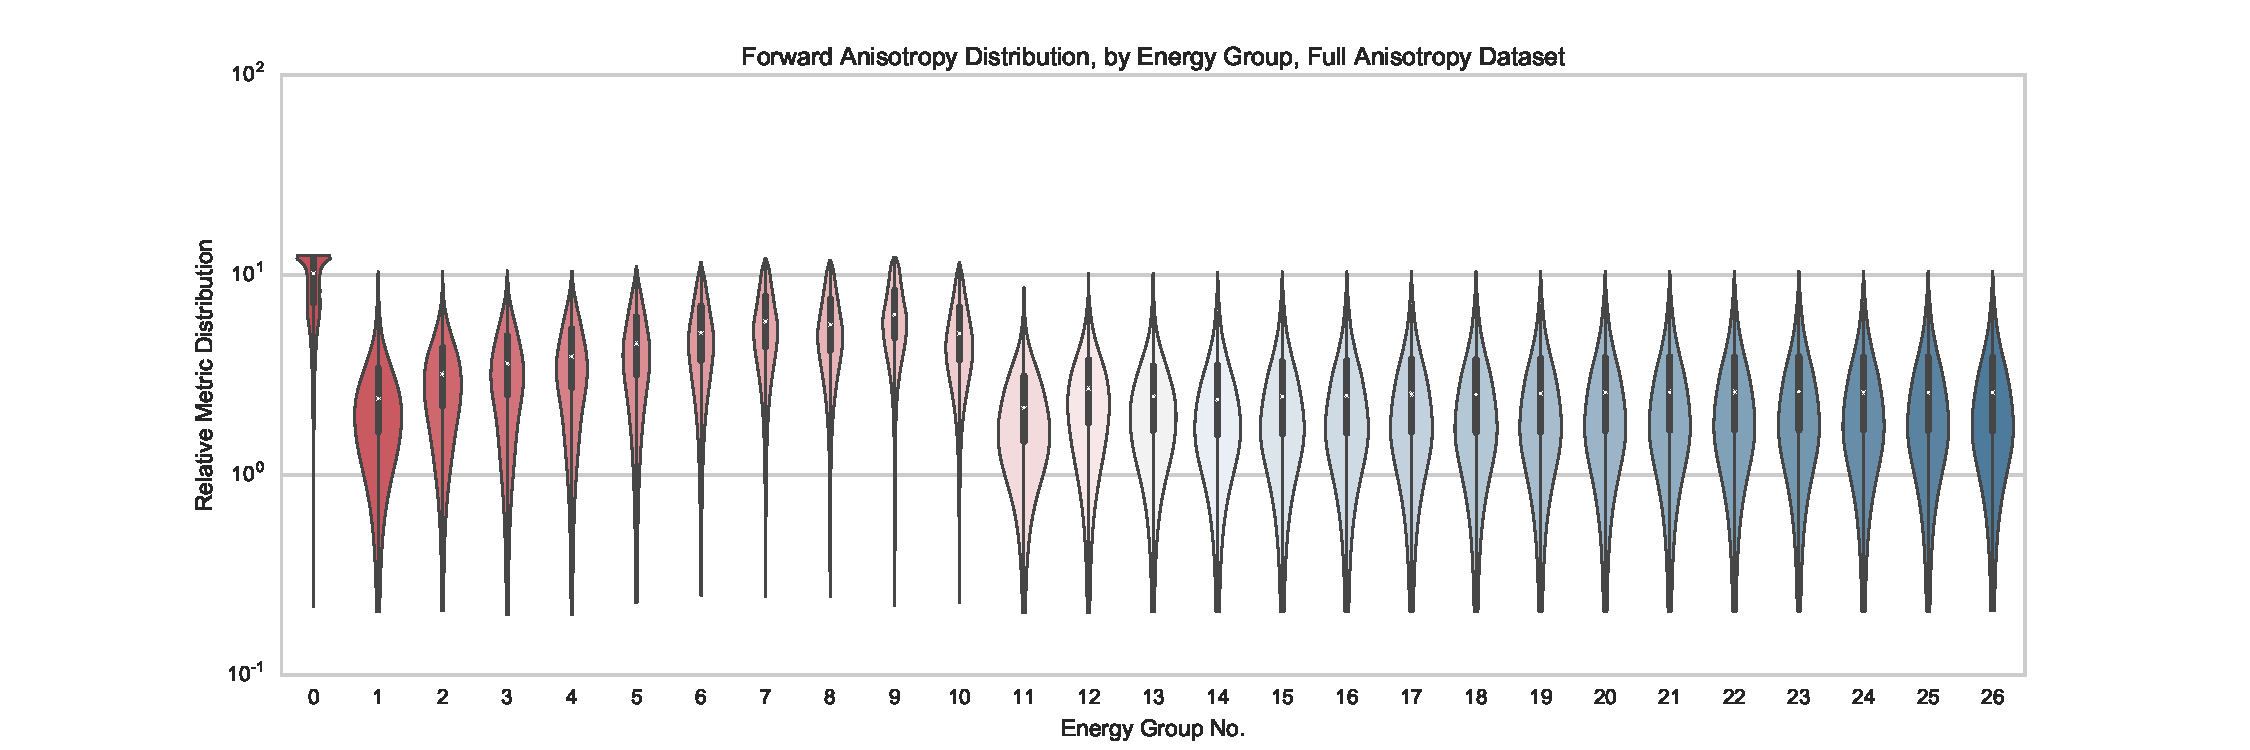
\includegraphics[width=\linewidth]{./chapters/characterization_probs/figures/char/beam/forward_anisotropy_violin_full.pdf}
    \caption{Full forward flux anisotropy distribution}
    \label{fig:forwardbeamline}
  \end{subfigure}
\end{figure}
\begin{figure}[htb!]\ContinuedFloat
  \centering
  \begin{subfigure}[t]{\textwidth}
    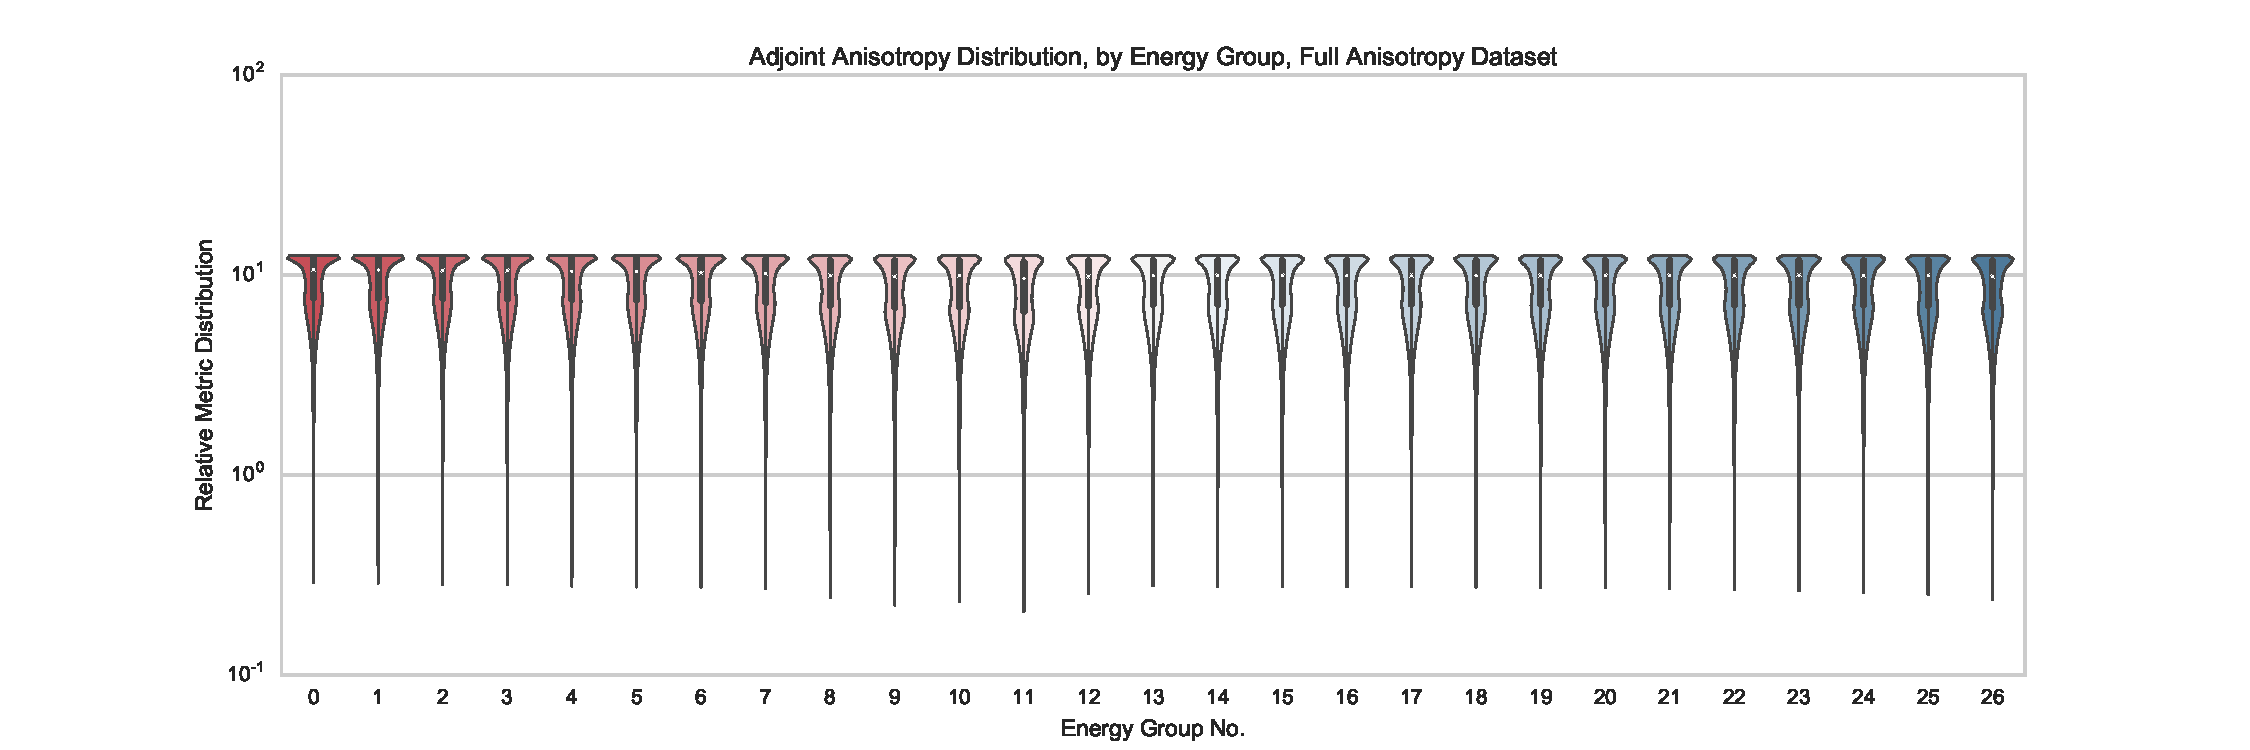
\includegraphics[width=\linewidth]{./chapters/characterization_probs/figures/char/beam/adjoint_anisotropy_violin_full.pdf}
    \caption{Full adjoint flux anisotropy distribution}
    \label{fig:adjointbeamline}
  \end{subfigure}
  \caption[Forward and adjoint anisotropy distributions for experimental
  nuclear physics beamline]{Forward and adjoint anisotropy distributions for
  experimental nuclear physics beamline.}
  \label{fig:beamlineplots}
\end{figure}

While this problem has very poor performance for the relative errors of CADIS
and CADIS-$\Omega$, some interesting physics can be highlighted by looking at
the distributions of the forward and adjoint anisotropy. Here the ratio of the
maximum angular flux to the average angular flux is computed for each cell.
Figure \ref{fig:forwardbeamline} shows the distribution of values for the
forward flux, and Figure \ref{fig:adjointbeamline} shows the distribution of
values for the adjoint flux. Because this value has extremely high leakage, we
can see the effect of moderation on the distributions. The forward flux in this
problem is defined as a monodirectional beam aimed at a NaI cube. As a result,
the highest energy group only exists in the problem between the source and the
cube. This is reflected in the very different distribution for the highest
energy group and all of the other energy groups.

Because all of the highest energy particles are removed--most likely by
downscattering to lower energies--from the problem after interacting with the
NaI cube, the distribution is dominated by the monodirectional beam. The
distribution of values in this energy group are strongly peaked towards a single
direction, which is the limiting upper value of group 0.

Compare the forward distributions of Figure \ref{fig:forwardbeamline} to the
adjoint distributions of Figure \ref{fig:adjointbeamline}. All energy groups
in the adjoint variant are similar to the fastest in the forward problem. This
is because the adjoint source particle distribution is not angle-dependent as it
is in the forward problem. The other NaI detector in the problem comprises a very
small fraction of the solid angle of the adjoint source. As a result, all energy
groups are fairly monodirectional, and particles stream out of the problem.

\subsection{Therapy Room}
\label{subsec:resultstherapy}

The problem with a simplified representation of a nuclear medicine therapy room
has FOM summarized in Table
\ref{tab:therapyfoms}. Figures
\ref{fig:therapyresult} and \ref{fig:therapyerror} show the results obtained
by the track length tally in CADIS, CADIS-$\Omega$ and the nonbiased analog
Monte Carlo. Note that the results for this problem had issues with reported
times for the deterministic run, so the adjusted Monte Carlo
(FOM$_{hybrid}$) is not reported and the timing table is not reported.

\begin{table}[h!]
  \centering
  \begin{tabular}{lrrrrr}
\toprule
{} & cadis &             & cadisangle &             & analog \\
{} &    MC & MC\_adjusted &         MC & MC\_adjusted &     MC \\
\midrule
tally avg   &  5.81 &        5.71 &        106 &        8.34 &   2.81 \\
max RE      & 0.463 &       0.455 &      0.822 &      0.0649 & 0.0136 \\
min RE      &  37.6 &          37 &       32.9 &         2.6 &  0.793 \\
time (mins) &  44.7 &        45.4 &       39.9 &         506 &    248 \\
\bottomrule
\end{tabular}

  \caption[Tally results comparison between methods for simplified medical
  therapy room.]{Tally relative error comparison between methods for simplified
  medical therapy room.}
  \label{tab:therapyfoms}
\end{table}

The therapy room is a problem where CADIS-$\Omega$ performs fairly well when
compared to CADIS and the nonbiased analog Monte Carlo. For the Monte Carlo
runtime-exclusive FOMs, CADIS-$\Omega$ achieves better FOMs than CADIS and the
nonbiased analog in both the tally average relative error and the tally maximum
relative error.

\begin{figure}[h!]
  \centering
  \includegraphics[height=10cm]{./chapters/characterization_probs/figures/char/therapy/therapy_room_tally_result_compare.pdf}
  \caption[Tally results comparison between methods for simplified medical
  therapy room.]
  {Tally results comparison between methods for simplified medical therapy room.}
  \label{fig:therapyresult}
\end{figure}

\begin{figure}[h!]
  \centering
  \includegraphics[height=10cm]{./chapters/characterization_probs/figures/char/therapy/therapy_room_tally_error_compare.pdf}
  \caption[Tally relative error comparison between methods for simplified
  medical therapy room.]
  {Tally relative error comparison between methods for simplified medical
  therapy room.}
  \label{fig:therapyerror}
\end{figure}

For this problem, CADIS-$\Omega$ achieved similar relative errors to CADIS for
intermediate- and fast- energy bins. However, for low energy bins CADIS
performed poorly and CADIS-$\Omega$ achieved satisfactory relative errors. These
low energy bins are the only ones where CADIS-$\Omega$ really substantially
outperformed CADIS. In a similar problem it would be advantageous to use
CADIS-$\Omega$ as a method, but with deterministic runtime incorporated it may
still be worthwhile to run with CADIS instead. If a user desires a tally with
low energy bins exclusively, CADIS-$\Omega$ will be the advantageous method.

